% Problems, Chapter 2: Boundary-Value Problems in Electrostatics: I
% Jackson, Classical Electrodynamics, 3rd ed.
% Requires: amsmath, amssymb, tikz

\section*{Problems}

\Needspace{5\baselineskip}
\par\bigskip
\noindent\textbf{2.1}\quad A point charge $q$ is brought to a position a distance $d$ away from an infinite plane conductor held at zero potential. Using the method of images, find:
\begin{enumerate}
\item[(a)] the surface-charge density induced on the plane, and plot it;
\item[(b)] the force between the plane and the charge by using Coulomb's law for the force between the charge and its image;
\item[(c)] the total force acting on the plane by integrating $\sigma^{2}/2\epsilon_{0}$ over the whole plane;
\item[(d)] the work necessary to remove the charge $q$ from its position to infinity;
\item[(e)] the potential energy between the charge $q$ and its image [compare the answer to part d and discuss].
\item[(f)] Find the answer to part d in electron volts for an electron originally one angstrom from the surface.
\end{enumerate}
\solution
Put the plane at $z=0$ and the real charge at $d\widehat{\mathbf z}$.
All potentials below refer to the vacuum region $z>0$; the image is
$-q$ at $-d\widehat{\mathbf z}$. Thus
\[
\Phi(\rho,z)=\frac{q}{4\pi\epsilon _0}
 \left[\frac1{\sqrt{\rho^2+(z-d)^2}}
       -\frac1{\sqrt{\rho^2+(z+d)^2}}\right].
\]
\textbf{(a)} The normal from the metal into the vacuum is
$\widehat{\mathbf z}$, so $\sigma=-\epsilon _0\partial_z\Phi|_{0^+}$.
Differentiating the two terms gives respectively
$d/(\rho^2+d^2)^{3/2}$ and $d/(\rho^2+d^2)^{3/2}$, whence
\[
\boxed{\sigma(\rho)=-\frac{qd}{2\pi(\rho^2+d^2)^{3/2}}.}
\]
As a normalization check,
$2\pi\int_0^\infty\sigma\rho\,d\rho
=-qd[-(\rho^2+d^2)^{-1/2}]_0^\infty=-q$.
The following plot uses $u=\rho/d$ and
$-2\pi d^2\sigma/q=(1+u^2)^{-3/2}$ (the signed density is negative
for $q>0$).
\begin{center}
\begin{tikzpicture}[x=1.05cm,y=2cm]
\draw[->] (0,0)--(5.2,0) node[right] {$\rho/d$};
\draw[->] (0,0)--(0,1.2) node[above] {$-2\pi d^2\sigma/q$};
\draw[thick,blue,domain=0:5,samples=100] plot (\x,{1/(1+\x*\x)^1.5});
\foreach \x in {1,2,3,4,5} \draw (\x,.025)--(\x,-.025) node[below] {$\x$};
\node[left] at (0,1) {$1$};
\end{tikzpicture}
\end{center}
\textbf{(b)} The separation of the charge and image is $2d$, hence
\[
\boxed{\mathbf F_q=-\frac{q^2}{16\pi\epsilon _0d^2}\widehat{\mathbf z}.}
\]
\textbf{(c)} The electrostatic pressure on the metal is toward the
vacuum. Its integral is
\begin{align*}
\mathbf F_{\rm plane}
&=\widehat{\mathbf z}\int_0^\infty
 \frac{q^2d^2}{8\pi^2\epsilon _0(\rho^2+d^2)^3}\,2\pi\rho\,d\rho\\
&=\widehat{\mathbf z}\frac{q^2d^2}{4\pi\epsilon _0}
 \left[-\frac1{4(\rho^2+d^2)^2}\right]_0^\infty
=\frac{q^2}{16\pi\epsilon _0d^2}\widehat{\mathbf z}.
\end{align*}
This equals $-\mathbf F_q$.
\textbf{(d)} In quasistatic removal the applied force opposes the
attraction at every instantaneous height $s$, so
\[
\boxed{W=\int_d^\infty\frac{q^2}{16\pi\epsilon _0s^2}\,ds
       =\frac{q^2}{16\pi\epsilon _0d}.}
\]
\textbf{(e)} Two \emph{independent} charges $q,-q$ a distance $2d$
apart have mutual energy $U_{q,q'}=-q^2/(8\pi\epsilon _0d)=-2W$.
The physical charge--conductor energy relative to infinite separation
is instead
\[
U=\frac12q\Phi_{\rm induced}(d)
 =-\frac{q^2}{16\pi\epsilon _0d}=-W.
\]
The factor $1/2$ follows by charging the real source from $0$ to $q$:
the induced potential is proportional to the charge already supplied,
so $U=\int_0^q(q_1/q)\Phi_{\rm induced}(q)\,dq_1$.
An image is a representation of this induced charge, not an additional
independently assembled physical source.
\textbf{(f)} With $|q|=e$, $d=10^{-10}\,\mathrm m$, the conversion is
\[
W[\mathrm{eV}]=\frac{e}{16\pi\epsilon _0(10^{-10}\,\mathrm m)}
\simeq\boxed{3.60\ \mathrm{eV}}.
\]
The numerical check uses the SI constants in \texttt{scipy.constants}.

\Needspace{5\baselineskip}
\par\bigskip
\noindent\textbf{2.2}\quad Using the method of images, discuss the problem of a point charge $q$ \emph{inside} a hollow, grounded, conducting sphere of inner radius $a$. Find
\begin{enumerate}
\item[(a)] the potential inside the sphere;
\item[(b)] the induced surface-charge density;
\item[(c)] the magnitude and direction of the force acting on $q$.
\item[(d)] Is there any change in the solution if the sphere is kept at a fixed potential $V$? If the sphere has a total charge $Q$ on its inner and outer surfaces?
\end{enumerate}
\solution
Let the charge be at $b\widehat{\mathbf z}$, $0<b<a$. Inversion in the
sphere gives an image $q'=-qa/b$ at $b'=a^2/b>a$. On $r=a$,
$|\mathbf r-b'\widehat{\mathbf z}|=(a/b)
 |\mathbf r-b\widehat{\mathbf z}|$, so their potentials cancel.
\textbf{(a)} By uniqueness,
\[
\boxed{\Phi(r,\theta)=\frac{q}{4\pi\epsilon _0}
 \left[\frac1{\sqrt{r^2+b^2-2rb\cos\theta}}
 -\frac{a/b}{\sqrt{r^2+a^4/b^2-2ra^2\cos\theta/b}}\right],\quad r<a.}
\]
The image lies outside the solution domain and creates no extra
singularity in the cavity.
\textbf{(b)} The metal-to-cavity normal is $-\widehat{\mathbf r}$,
so $\sigma=\epsilon _0\partial_r\Phi|_{a^-}$. To simplify the derivative,
write $D=\sqrt{a^2+b^2-2ab\cos\theta}$ and use the distance relation:
\[
\partial_r\Phi|_a=\frac{q}{4\pi\epsilon _0D^3}
 \left[-(a-b\cos\theta)+\frac{b^2}{a^2}
              \left(a-\frac{a^2}{b}\cos\theta\right)\right].
\]
Thus
\[
\boxed{\sigma(\theta)=-\frac{q(a^2-b^2)}
 {4\pi a(a^2+b^2-2ab\cos\theta)^{3/2}}.}
\]
Indeed, setting $u=\cos\theta$ gives
\[
2\pi a^2\int_{-1}^1\sigma(u)\,du
=-\frac{qa(a^2-b^2)}2\frac1{ab}
 \left(\frac1{a-b}-\frac1{a+b}\right)=-q.
\]
\textbf{(c)} Only the image field acts on $q$ after its own singular
field is excluded. The distance is $b'-b=(a^2-b^2)/b$, giving
\[
\boxed{\mathbf F=\frac{q^2ab}{4\pi\epsilon _0(a^2-b^2)^2}
                    \widehat{\mathbf z}.}
\]
It is toward the nearer wall for either sign of $q$.
For a centered charge the limits are
$\Phi=q(1/r-1/a)/(4\pi\epsilon _0)$,
$\sigma=-q/(4\pi a^2)$, and $\mathbf F=0$.
\textbf{(d)} Holding the metal at $V$ adds the constant $V$ to the
cavity potential; it leaves the cavity field, inner surface charge,
and force unchanged. For an isolated metal with total charge $Q$,
Gauss's law in the metal requires inner charge $-q$ and outer charge
$Q+q$. The same cavity solution therefore holds up to a constant.
That constant depends on the exterior geometry. For a concentric
spherical outer surface of radius $A$, with no other external sources
and zero potential at infinity, it is $(Q+q)/(4\pi\epsilon _0A)$.
For an ideal thin shell one sets $A=a$. Specifying only the inner
radius does not specify this exterior capacitance.

\Needspace{5\baselineskip}
\par\bigskip
\noindent\textbf{2.3}\quad A straight-line charge with constant linear charge density $\lambda$ is located perpendicular to the $x$-$y$ plane in the first quadrant at $(x_{0},y_{0})$. The intersecting planes $x=0$, $y\geq0$ and $y=0$, $x\geq0$ are conducting boundary surfaces held at zero potential. Consider the potential, fields, and surface charges in the first quadrant.
\begin{enumerate}
\item[(a)] The well-known potential for an isolated line charge at $(x_{0},y_{0})$ is $\Phi(x,y)=(\lambda/4\pi\epsilon_{0})\ln(R^{2}/r^{2})$, where $r^{2}=(x-x_{0})^{2}+(y-y_{0})^{2}$ and $R$ is a constant. Determine the expression for the potential of the line charge in the presence of the intersecting planes. Verify explicitly that the potential and the tangential electric field vanish on the boundary surfaces.
\item[(b)] Determine the surface charge density $\sigma$ on the plane $y=0$, $x\geq0$. Plot $\sigma/\lambda$ versus $x$ for $(x_{0}=2,y_{0}=1)$, $(x_{0}=1,y_{0}=1)$, and $(x_{0}=1,y_{0}=2)$.
\item[(c)] Show that the total charge (per unit length in $z$) on the plane $y=0$, $x\geq0$ is
\[
Q_{x} = -\frac{2}{\pi}\lambda\tan^{-1}\!\left(\frac{x_{0}}{y_{0}}\right)
\]
What is the total charge on the plane $x=0$?
\item[(d)] Show that far from the origin [$\rho\gg\rho_{0}$, where $\rho=\sqrt{x^{2}+y^{2}}$ and $\rho_{0}=\sqrt{x_{0}^{2}+y_{0}^{2}}$] the leading term in the potential is
\[
\Phi\rightarrow\Phi_{\mathrm{asym}}=\frac{4\lambda}{\pi\epsilon_{0}}\frac{(x_{0}y_{0})(xy)}{\rho^{4}}
\]
Interpret.
\end{enumerate}
\solution
Define $D_{st}=(x-sx_0)^2+(y-ty_0)^2$, with $s,t=\pm1$.
\textbf{(a)} Place line charges $st\lambda$ at $(sx_0,ty_0)$.
The arbitrary logarithmic reference lengths cancel because the
four charges sum to zero, leaving
\[
\boxed{\Phi=\frac{\lambda}{4\pi\epsilon _0}
 \ln\frac{D_{+-}D_{-+}}{D_{++}D_{--}}.}
\]
At $y=0$, $D_{++}=D_{+-}$ and $D_{-+}=D_{--}$, so $\Phi=0$;
at $x=0$ the other two equalities give the same result. Differentiating
these identities along either boundary gives $E_x(x,0)=0$ and
$E_y(0,y)=0$. All terms are independent of $z$, so $E_z=0$ as well.
\textbf{(b)} On $y=0$ the outward metal normal is $+\widehat{\mathbf y}$.
Differentiating the logarithms before putting $y=0$ gives
\[
\boxed{\frac{\sigma(x)}\lambda=-\frac{y_0}{\pi}
 \left[\frac1{(x-x_0)^2+y_0^2}-\frac1{(x+x_0)^2+y_0^2}\right].}
\]
It vanishes at the corner, is negative for $x>0$ when $\lambda>0$,
and decays as $-4x_0y_0/(\pi x^3)$.
\begin{center}
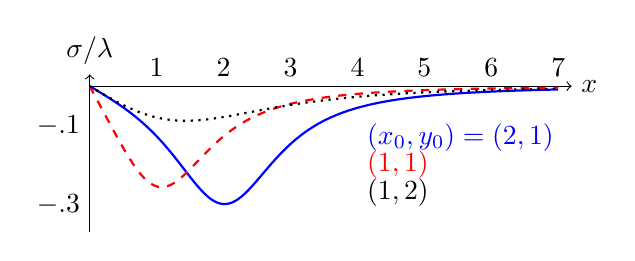
\begin{tikzpicture}[x=.85cm,y=5cm]
\draw[->] (0,0)--(7.2,0) node[right] {$x$};
\draw[->] (0,-.37)--(0,.03) node[above] {$\sigma/\lambda$};
\draw[blue,thick,domain=0:7,samples=140]
 plot (\x,{-1/pi*(1/((\x-2)^2+1)-1/((\x+2)^2+1))});
\draw[red,dashed,thick,domain=0:7,samples=140]
 plot (\x,{-1/pi*(1/((\x-1)^2+1)-1/((\x+1)^2+1))});
\draw[black,dotted,thick,domain=0:7,samples=140]
 plot (\x,{-2/pi*(1/((\x-1)^2+4)-1/((\x+1)^2+4))});
\foreach \x in {1,2,3,4,5,6,7} \node[above] at (\x,0) {$\x$};
\node[left] at (0,-.1) {$-.1$}; \node[left] at (0,-.3) {$-.3$};
\node[blue,right] at (4,-.13) {$(x_0,y_0)=(2,1)$};
\node[red,right] at (4,-.20) {$(1,1)$};
\node[right] at (4,-.27) {$(1,2)$};
\end{tikzpicture}
\end{center}
\textbf{(c)} Integrating each Lorentzian explicitly,
\begin{align*}
Q_x&=-\frac\lambda\pi
 \left[\tan^{-1}\frac{x-x_0}{y_0}
       -\tan^{-1}\frac{x+x_0}{y_0}\right]_{x=0}^{\infty}\\
&=\boxed{-\frac{2\lambda}{\pi}\tan^{-1}\frac{x_0}{y_0}}.
\end{align*}
Interchange $x_0,y_0$ for the other plane:
$Q_y=-2\lambda\tan^{-1}(y_0/x_0)/\pi$.
Since both coordinates are positive, their inverse tangents add to
$\pi/2$ and $Q_x+Q_y=-\lambda$.
\textbf{(d)} Write $D_{st}=\rho^2+B_{st}$, with
$B_{st}=\rho_0^2-2sxx_0-2tyy_0$. In
$\Phi=-\lambda\sum st\ln D_{st}/(4\pi\epsilon _0)$,
the constant and first-order terms cancel. The needed quadratic sum is
\[
\sum_{s,t}st B_{st}^2=32xx_0yy_0,
\quad
\sum_{s,t}st\ln D_{st}=-\frac{16xx_0yy_0}{\rho^4}
 +O(\rho_0^4/\rho^4).
\]
Consequently
\[
\boxed{\Phi\sim\frac{4\lambda x_0y_0xy}{\pi\epsilon _0\rho^4}.}
\]
The images cancel both the net line charge and the dipole moment.
This is the leading two-dimensional quadrupole, proportional to
$\sin2\phi/\rho^2$, with nodes on the grounded planes.

\Needspace{5\baselineskip}
\par\bigskip
\noindent\textbf{2.4}\quad A point charge is placed a distance $d>R$ from the center of an equally charged, isolated, conducting sphere of radius $R$.
\begin{enumerate}
\item[(a)] Inside of what distance from the surface of the sphere is the point charge attracted rather than repelled by the charged sphere?
\item[(b)] What is the limiting value of the force of attraction when the point charge is located a distance $a$ ($=d-R$) from the surface of the sphere, if $a\ll R$?
\item[(c)] What are the results for parts a and b if the charge on the sphere is twice (half) as large as the point charge, but still the same sign?
\end{enumerate}
[Answers: (a) $d/R-1=\erratum{0.6180}$, (b) $F=-q^{2}/(16\pi\epsilon_{0}a^{2})$, i.e., image force, (c) for $Q=2q$, $d/R-1=0.4276$; for $Q=q/2$, $d/R-1=0.8823$. The answer for part b is the same.]
\solution
Let $k=(4\pi\epsilon _0)^{-1}$ and write $Q=\alpha q$ for the sphere's
charge. The image pair inside the sphere is
\[
q'=-\frac{qR}{d},\quad r'=\frac{R^2}{d},\qquad
q_0=Q+\frac{qR}{d}\quad\hbox{at the center}.
\]
The image $q'$ cancels the angular variation on the surface and the
central charge makes the total image charge $Q$. Taking positive force
away from the center,
\[
F=kq\left[\frac{Q+qR/d}{d^2}
       -\frac{qR/d}{(d-R^2/d)^2}\right]
=\frac{kq^2}{R^2}\left[\frac{\alpha+1/x}{x^2}
                  -\frac{x}{(x^2-1)^2}\right],\quad x=\frac dR.
\]
\textbf{(a)} Setting $F=0$ is equivalent to
\[
\alpha=H(x):=\frac{2x^2-1}{x(x^2-1)^2}.
\]
For $x>1$,
$H'(x)=(-6x^4+3x^2-1)/[x^2(x^2-1)^3]<0$;
also $H(1^+)=\infty$ and $H(\infty)=0$. There is exactly one root,
with attraction below it. For $\alpha=1$ the root is
$x=(1+\sqrt5)/2$: using $x^2=x+1$ makes both sides of
$x(x^2-1)^2=2x^2-1$ equal $2x+1$. Thus
\[
\boxed{0<d-R<\frac{\sqrt5-1}{2}R=0.6180339887\ldots R.}
\]
This exact root, rounded to four figures, is the corrected answer
marked in the statement.
\textbf{(b)} Set $d=R+a$. Then
$d-R^2/d=2a+O(a^2/R)$ and $q'=-q+O(qa/R)$,
whereas the central-charge force remains finite. Therefore
\[
\boxed{F\sim-\frac{kq^2}{4a^2}
            =-\frac{q^2}{16\pi\epsilon _0a^2}\quad(a/R\to0).}
\]
\textbf{(c)} Solving the same monotone equation $H(x)=\alpha$ gives
\[
\begin{array}{c|c|c}
Q/q&x\text{ at zero force}&(d-R)/R\text{ at zero force}\\\hline
2&1.427563934\ldots&0.427563934\ldots\\
1/2&1.882269146\ldots&0.882269146\ldots
\end{array}
\]
Attraction holds below these respective distances. The leading
near-surface force in part (b) is independent of the finite value of
$Q/q$ because it comes from the nearby image.

\Needspace{5\baselineskip}
\par\bigskip
\noindent\textbf{2.5}\quad\begin{enumerate}
\item[(a)] Show that the work done to remove the charge $q$ from a distance $r>a$ to infinity against the force, Eq.~(2.6), of a grounded conducting sphere is
\[
W=\frac{q^{2}a}{8\pi\epsilon_{0}(r^{2}-a^{2})}
\]
Relate this result to the electrostatic potential, Eq.~(2.3), and the energy discussion of Section 1.11.
\item[(b)] Repeat the calculation of the work done to remove the charge $q$ against the force, Eq.~(2.9), of an isolated charged conducting sphere. Show that the work done is
\[
W=\frac{1}{4\pi\epsilon_{0}}\left[\frac{q^{2}a}{2(r^{2}-a^{2})}-\frac{q^{2}a}{2r^{2}}-\frac{qQ}{r}\right]
\]
Relate the work to the electrostatic potential, Eq.~(2.8), and the energy discussion of Section 1.11.
\end{enumerate}
\solution
Use $k=(4\pi\epsilon _0)^{-1}$ and take outward force as positive.
\textbf{(a)} The grounded-sphere image at a source position $s>a$ is
$-qa/s$ at $a^2/s$. Hence the force appearing in (2.6) is
\[
F_g(s)=-k\frac{q^2a/s}{(s-a^2/s)^2}
       =-k\frac{q^2as}{(s^2-a^2)^2}.
\]
The quasistatic work is
\[
W_g=-\int_r^\infty F_g(s)\,ds
=kq^2a\left[-\frac1{2(s^2-a^2)}\right]_r^\infty
=\boxed{\frac{q^2a}{8\pi\epsilon _0(r^2-a^2)}}.
\]
At the source the induced potential from the image construction
of (2.3) is $\Phi_{\rm ind}=-kqa/(r^2-a^2)$.
Therefore $U_g=\tfrac12q\Phi_{\rm ind}=-W_g$.
The half factor is the work of building up the induced charge
linearly with the real source, as in Section 1.11, with the divergent
self-energy of the point charge omitted.
\textbf{(b)} For an isolated sphere, add a central charge
$Q+qa/s$ to the grounded image. Thus the force (2.9) is
\[
F_Q(s)=-k\frac{q^2as}{(s^2-a^2)^2}
        +k\frac{qQ}{s^2}+k\frac{q^2a}{s^3}.
\]
Termwise integration gives
\begin{align*}
W_Q&=-\int_r^\infty F_Q(s)\,ds\\
&=\boxed{k\left[\frac{q^2a}{2(r^2-a^2)}
              -\frac{q^2a}{2r^2}-\frac{qQ}{r}\right]}.
\end{align*}
This work can be negative when repulsion supplies energy during
removal. To see the energy content of (2.8), separate the potential at
$q$ into the pre-existing charge and the polarization:
\[
\Phi_Q(r)=\frac{kQ}{r},\qquad
\Phi_{\rm pol}(r)=kq\left[\frac{a}{r^2}-\frac{a}{r^2-a^2}\right].
\]
Relative to the infinitely separated system, the energy is
\[
U_Q=q\Phi_Q+\frac12q\Phi_{\rm pol}=-W_Q.
\]
The pre-existing sphere charge $Q$ has its full interaction factor;
only the source-induced redistribution has the half factor.
The constant self-energy $kQ^2/(2a)$ of the isolated charged sphere
cancels between the initial and final configurations.

\Needspace{5\baselineskip}
\par\bigskip
\noindent\textbf{2.6}\quad The electrostatic problem of a point charge $q$ outside an isolated, charged conducting sphere is equivalent to that of three charges, the original and two others, one located at the center of the sphere and another (``the image charge'') inside the now imaginary sphere, on the line joining the center and the original charge.

If the point charge and sphere are replaced by two conducting spheres of radii $r_{a}$ and $r_{b}$, carrying total charges $Q_{a}$ and $Q_{b}$, respectively, with centers separated by a distance $d>r_{a}+r_{b}$, there is an equivalence with an infinite set of charges within each sphere, one at the center and a set of images along the line joining the centers. The charges and their locations can be determined iteratively, starting with a charge $q_{a}(1)$ at the center of the first sphere and $q_{b}(1)$ correspondingly for the second sphere. The charge $q_{b}(1)$ has its image $q_{a}(2)$ within the first sphere and vice versa. Then the image charge within the first sphere induces another image within the second sphere, and so on. The sum of all the charges within each sphere must be scaled to be equal to $Q_{a}$ or $Q_{b}$.

The electrostatic potential outside the spheres, the force between the spheres, etc. can be found by summing the contributions from all the charges.
\begin{enumerate}
\item[(a)] Show that the charges and their positions are determined iteratively by the relations,
\begin{align*}
q_{a}(j)&=-r_{a}q_{b}(j-1)/d_{b}(j-1), & x_{a}(j)&=r_{a}^{2}/d_{b}(j-1), & d_{a}(j)&=d-x_{a}(j)\\
q_{b}(j)&=-r_{b}q_{a}(j-1)/d_{a}(j-1), & x_{b}(j)&=r_{b}^{2}/d_{a}(j-1), & d_{b}(j)&=d-x_{b}(j)
\end{align*}
for $j=2,3,4,\ldots$, with $d_{a}(1)=d_{b}(1)=d$, and $x_{a}(1)=x_{b}(1)=0$.
\item[(b)] Find the image charges and their locations as well as the potentials on the spheres and force between them by means of a suitable computer program. [In computing the potential on each sphere, evaluate it in different places: e.g., in the equatorial plane and at the pole opposite the other sphere. This permits a check on the equipotential of the conductor and on the accuracy of computation.]
\item[(c)] As an example, show that for two equally charged spheres of the same radius $R$, the force between them when almost in contact is \erratum{0.6149} times the value that would be obtained if all the charge on each sphere were concentrated at its center. Show numerically and by explicit summation of the series that the capacitance of two identical conducting spheres in contact is $C/4\pi\epsilon_{0}R=1.3863\cdots$ [$=\ln4$].
\end{enumerate}
Reference: J. A. Soules, \emph{Am. J. Phys.} \textbf{58}, 1195 (1990).
\solution
Use an axial coordinate $X$ with centers at $0,d$. Distances $x_a$
and $x_b$ are measured from each center \emph{toward} the other, so
charges in sphere $b$ have global coordinates $d-x_b$.
\textbf{(a)} A charge $q_b(j-1)$ is a distance
$d_b(j-1)=d-x_b(j-1)>r_a$ from center $a$. Sphere inversion therefore
requires an image
\[
q_a(j)=-\frac{r_a}{d_b(j-1)}q_b(j-1),\qquad
x_a(j)=\frac{r_a^2}{d_b(j-1)}.
\]
Interchanging $a,b$ gives the other two recurrences in the question.
Every external image is paired with its cancelling image in the
other sphere. On sphere $a$ these pairs have zero potential, leaving
only the central charge's constant $kq_a(1)/r_a$; similarly on $b$.
The two initial charges cannot in general be scaled independently
after the iteration, because each subsequent chain crosses between
the spheres.

\textbf{(b)} A reproducible implementation is the function
\texttt{two\_spheres} in the supplementary script
\texttt{check\_ch02.py}.
It first constructs two unit-seed solutions, with initial central
charges $(1,0)$ and $(0,1)$. If $M_{ij}$ is the sum of the images
in sphere $i$ produced by seed $j$, solve
\[
\begin{pmatrix}M_{aa}&M_{ab}\\M_{ba}&M_{bb}\end{pmatrix}
\begin{pmatrix}q_a(1)\\q_b(1)\end{pmatrix}
=\begin{pmatrix}Q_a\\Q_b\end{pmatrix}.
\]
In particular, writing $\Delta=M_{aa}M_{bb}-M_{ab}M_{ba}$,
\[
q_a(1)=\frac{Q_aM_{bb}-Q_bM_{ab}}\Delta,\qquad
q_b(1)=\frac{Q_bM_{aa}-Q_aM_{ba}}\Delta.
\]
If the two stored unit-seed charges at a given image position are
$c_{i,a}(j),c_{i,b}(j)$, its final charge is
$q_i(j)=c_{i,a}(j)q_a(1)+c_{i,b}(j)q_b(1)$.
Linearity then gives every image charge at the already computed
positions. For a finite truncation the exterior potential and the
outward force on sphere $b$ are evaluated as
\begin{align*}
\Phi(X,\rho)&=k\sum_j\left[
 \frac{q_a(j)}{\sqrt{(X-x_a(j))^2+\rho^2}}
+\frac{q_b(j)}{\sqrt{(X-d+x_b(j))^2+\rho^2}}\right],\\
F_b&=k\sum_{i,j}\frac{q_a(i)q_b(j)}{[d-x_a(i)-x_b(j)]^2}.
\end{align*}
The latter follows by enclosing one sphere in a Maxwell-stress
surface: its self-field gives zero net force, and the interaction
with the other sphere can be replaced by the two sets of images.
For a strictly positive gap, every successive image magnitude is
bounded by the previous magnitude times
\[
\eta=\max\left(\frac{r_a}{d-r_b},\frac{r_b}{d-r_a}\right)<1,
\]
because each image remains inside its sphere. If $c_N$ bounds the
last retained charge in either unit-seed chain, each remaining tail
is at most $c_N\eta/(1-\eta)$. After combining the seeds this is
multiplied by $|q_a(1)|+|q_b(1)|$. The code increases the image count
until the unit-seed bound meets the requested tolerance and reports
the resulting physical bound. Its checks repeat the calculation at a tighter tolerance,
compare the resulting force and potentials, and compare each surface
potential at the facing pole, rear pole, and equator with
$V_i=kq_i(1)/r_i$. It exposes all charges
and positions in the returned arrays and can write them to a CSV
file using \texttt{--images PATH}.
For example, $r_a=r_b=R$, $d=3R$, $Q_a=Q_b=Q$ gives
\[
\frac{4\pi\epsilon _0RV}{Q}=1.320647\ldots,\qquad
\frac{F}{Q^2/(4\pi\epsilon _0d^2)}=0.849932\ldots.
\]
The script prints higher-precision values and includes an unequal
radius, unequal charge example to check the two-seed construction.

\textbf{(c)} For equal radii and equal charges put
$d=2R\cosh\alpha$, $\alpha>0$. The recurrences are solved by
\[
x_j=R\frac{\sinh[(j-1)\alpha]}{\sinh(j\alpha)},\qquad
q_j=(-1)^{j-1}q_1\frac{\sinh\alpha}{\sinh(j\alpha)}.
\]
For example,
$d-x_{j-1}=R\sinh(j\alpha)/\sinh[(j-1)\alpha]$
by $2\cosh\alpha\sinh[(j-1)\alpha]-\sinh[(j-2)\alpha]
=\sinh(j\alpha)$, which verifies both recurrences. Define
\[
S(\alpha)=\frac Q{q_1}
=\sinh\alpha\sum_{j=1}^{\infty}\frac{(-1)^{j-1}}{\sinh(j\alpha)}.
\]
Then $V=kQ/(RS)$ and the capacitance of the pair at a common
potential is
\[
\frac{C}{4\pi\epsilon _0R}=2S(\alpha).
\]
At contact the images become
$x_j=R(j-1)/j$, $q_j=(-1)^{j-1}q_1/j$, and therefore
\[
Q=q_1\left(1-\frac12+\frac13-\cdots\right)=q_1\ln2,
\qquad \boxed{\frac{C}{4\pi\epsilon _0R}=2\ln2=\ln4}.
\]
To differentiate near contact without differentiating a divergent
termwise power expansion, first sum a geometric series:
\[
S=2\sinh\alpha\sum_{m=0}^{\infty}\frac1{e^{(2m+1)\alpha}+1}.
\]
For $f(t)=(e^t+1)^{-1}$, midpoint summation gives
$h\sum_{m\geq0}f((m+\tfrac12)h)
=\int_0^\infty f(t)\,dt+h^2f'(0)/24+O(h^4)$.
This follows by integrating the Taylor expansion on each interval:
its midpoint error is $h^3f''/24$, whose sum is
$h^2\int_0^\infty f''/24=-h^2f'(0)/24$.
With $h=2\alpha$, $\int_0^\infty f=\ln2$ and $f'(0)=-1/4$, we find
\[
S=\ln2+\alpha^2\left(\frac{\ln2}{6}-\frac1{24}\right)+O(\alpha^4).
\]
At fixed charge on each sphere the total energy is
$U=\tfrac12(QV+QV)=kQ^2/(RS)$. Hence
\[
F=-\frac{dU}{dd}=\frac{kQ^2}{RS^2}\frac{dS}{dd},\qquad
 d=2R+R\alpha^2+O(\alpha^4).
\]
Dividing by the center-charge force $kQ^2/d^2$ gives the limit
\[
\boxed{\lim_{d\downarrow2R}\frac{F}{kQ^2/d^2}
=\frac{4\ln2-1}{6(\ln2)^2}=0.6149018638\ldots.}
\]
The printed value $0.6189$ is inconsistent with this exact limit; the
corrected value is $0.6149$. For example, at $(d-2R)/R=10^{-4}$ the
image-force ratio is $0.6149340086$, while the capacitance ratio is
$1.3863091325$, approaching $\ln4=1.3862943611$.
The supplementary code checks the image-force sum against both a
Maxwell-stress integral and the energy derivative, and approaches
both contact limits from positive gaps;
it does not rely on a finite alternating sum at exact contact.

\Needspace{5\baselineskip}
\par\bigskip
\noindent\textbf{2.7}\quad Consider a potential problem in the half-space defined by $z\geq0$, with Dirichlet boundary conditions on the plane $z=0$ (and at infinity).
\begin{enumerate}
\item[(a)] Write down the appropriate Green function $G(\mathbf{x},\mathbf{x}')$.
\item[(b)] If the potential on the plane $z=0$ is specified to be $\Phi=V$ \emph{inside} a circle of radius $a$ centered at the origin, and $\Phi=0$ outside that circle, find an integral expression for the potential at the point $P$ specified in terms of cylindrical coordinates $(\rho,\phi,z)$.
\item[(c)] Show that, along the axis of the circle ($\rho=0$), the potential is given by
\[
\Phi = V\!\left(1-\frac{z}{\sqrt{a^{2}+z^{2}}}\right)
\]
\item[(d)] Show that at large distances ($\rho^{2}+z^{2}\gg a^{2}$) the potential can be expanded in a power series in $(\rho^{2}+z^{2})^{-1}$, and that the leading terms are
\[
\Phi = \frac{Va^{2}}{2}\frac{z}{(\rho^{2}+z^{2})^{3/2}}\left[1-\frac{3a^{2}}{4(\rho^{2}+z^{2})}+\frac{5(3\rho^{2}a^{2}+a^{4})}{8(\rho^{2}+z^{2})^{2}}+\cdots\right]
\]
Verify that the results of parts c and d are consistent with each other in their common range of validity.
\end{enumerate}
\solution
Use the convention $\nabla'^2G=-4\pi\delta^3(\mathbf x-\mathbf x')$.
\textbf{(a)} Reflect the source in $z'=0$:
\[
\boxed{G(\mathbf x,\mathbf x')=
 \frac1{\sqrt{|\boldsymbol\rho-\boldsymbol\rho'|^2+(z-z')^2}}
-\frac1{\sqrt{|\boldsymbol\rho-\boldsymbol\rho'|^2+(z+z')^2}}.}
\]
It vanishes on the plane and at infinity. The outward normal of
the upper half-space is $-\widehat{\mathbf z}'$, giving
$\partial_{n'}G|_0=-2z/(|\boldsymbol\rho-\boldsymbol\rho'|^2+z^2)^{3/2}$.
\textbf{(b)} The Dirichlet representation
$\Phi=-(4\pi)^{-1}\int\Phi\partial_{n'}G\,dS'$ therefore yields
\[
\boxed{\Phi(\rho,z)=\frac{Vz}{2\pi}
 \int_0^a s\,ds\int_0^{2\pi}
 \frac{d\varphi}{(\rho^2+s^2-2\rho s\cos\varphi+z^2)^{3/2}}.}
\]
The result is independent of the observation azimuth.
\textbf{(c)} At $\rho=0$ the angular integral is $2\pi$, so
\[
\Phi(0,z)=Vz\left[-\frac1{\sqrt{s^2+z^2}}\right]_0^a
=\boxed{V\left(1-\frac z{\sqrt{a^2+z^2}}\right)},\qquad z>0.
\]
\textbf{(d)} Put $L^2=\rho^2+z^2$ and
$u=(s^2-2\rho s\cos\varphi)/L^2$. The binomial expansion is
$(1+u)^{-3/2}=1-3u/2+15u^2/8-35u^3/16+\cdots$.
A disk average, $\langle f\rangle=(\pi a^2)^{-1}\int s\,ds\,d\varphi f$,
gives
\[
\langle u\rangle=\frac{a^2}{2L^2},\qquad
\langle u^2\rangle=\frac{a^4/3+\rho^2a^2}{L^4}.
\]
Here $\langle s^2\rangle=a^2/2$,
$\langle s^4\rangle=a^4/3$, and
$\langle s^2\cos^2\varphi\rangle=a^2/4$.
Substitution produces the displayed denominator expansion:
\[
\Phi=\frac{Va^2z}{2L^3}
 \left[1-\frac{3a^2}{4L^2}
       +\frac{5(3\rho^2a^2+a^4)}{8L^4}+\cdots\right].
\]
For clarity, terms grouped by \emph{uniform far-distance order}
require some further terms from the binomial series, since
$\rho$ can be comparable to $L$. With $s_\theta=\rho/L$, that ordering is
\[
\Phi=\frac{Va^2z}{2L^3}\left\{
1+\frac{a^2}{L^2}\left(-\frac34+\frac{15}{8}s_\theta^2\right)
+\frac{a^4}{L^4}\left(\frac58-\frac{35}{8}s_\theta^2
                         +\frac{315}{64}s_\theta^4\right)
+O(a^6/L^6)\right\}.
\]
For example, the additional contributions at this order follow from
$\langle u^3\rangle=(a^6/4+2\rho^2a^4)/L^6$ and the
$2\rho^4a^4/L^8$ part of $\langle u^4\rangle$.
On the axis the original bracket becomes
$1-3a^2/(4z^2)+5a^4/(8z^4)+\cdots$, which agrees term by term with
$V[1-(1+a^2/z^2)^{-1/2}]$ from part (c).

\Needspace{5\baselineskip}
\par\bigskip
\noindent\textbf{2.8}\quad A two-dimensional potential problem is defined by two straight parallel line charges separated by a distance $R$ with equal and opposite linear charge densities $\lambda$ and $-\lambda$.
\begin{enumerate}
\item[(a)] Show by direct construction that the surface of constant potential $V$ is a circular cylinder (circle in the transverse dimensions) and find the coordinates of the axis of the cylinder and its radius in terms of $R$, $\lambda$, and $V$.
\item[(b)] Use the results of part a to show that the capacitance per unit length $C$ of two right-circular cylindrical conductors, with radii $a$ and $b$, separated by a distance $d>a+b$, is
\[
C=\frac{2\pi\epsilon_{0}}{\cosh^{-1}\!\left(\dfrac{d^{2}-a^{2}-b^{2}}{2ab}\right)}
\]
\item[(c)] Verify that the result for $C$ agrees with the answer in Problem 1.7 in the appropriate limit and determine the next nonvanishing order correction in powers of $a/d$ and $b/d$.
\item[(d)] Repeat the calculation of the capacitance per unit length for two cylinders inside each other ($d<|b-a|$). Check the result for concentric cylinders ($d=0$).
\end{enumerate}
\solution
\textbf{(a)} Put $+\lambda$ at $(c,0)$ and $-\lambda$ at $(-c,0)$,
where $c=R/2$, and choose zero potential at infinity. Then
\[
\Phi=\frac{\lambda}{4\pi\epsilon _0}
 \ln\frac{(x+c)^2+y^2}{(x-c)^2+y^2}.
\]
Set $t=2\pi\epsilon _0V/\lambda$. The equipotential equation is
$(x+c)^2+y^2=e^{2t}[(x-c)^2+y^2]$.
Dividing by $1-e^{2t}$ and completing the square yields
\[
\boxed{(x-c\coth t)^2+y^2=\frac{c^2}{\sinh^2t}.}
\]
Thus the cylinder axis passes through $(c\coth t,0)$ and its radius
is $c/|\sinh t|$. The exceptional level $V=0$ is the plane $x=0$
(the infinite-radius limit of the circles).
\textbf{(b)} For two disjoint cylinders choose their surfaces to be
$t=t_a>0$ and $t=-t_b<0$. Then
\[
a=c\,\mathrm{csch}\,t_a,\quad b=c\,\mathrm{csch}\,t_b,
\quad d=c(\coth t_a+\coth t_b).
\]
Squaring the last relation and using $\coth^2t-\mathrm{csch}^2t=1$
gives
\[
\frac{d^2-a^2-b^2}{2ab}
=\sinh t_a\sinh t_b+\cosh t_a\cosh t_b
=\cosh(t_a+t_b).
\]
Each cylinder encloses one of the two line charges, so Gauss's law
gives charges per unit length $\pm\lambda$. Their voltage difference
is $\Delta V=\lambda(t_a+t_b)/(2\pi\epsilon _0)$; therefore
\[
\boxed{C=\frac{\lambda}{\Delta V}
 =\frac{2\pi\epsilon _0}
 {\cosh^{-1}[(d^2-a^2-b^2)/(2ab)]}.}
\]
\textbf{(c)} Write $L=\ln[d^2/(ab)]$ and $S=a^2+b^2$.
For large $X$, $\cosh^{-1}X=\ln(2X)-1/(4X^2)+O(X^{-4})$;
substitution of $X=(d^2-S)/(2ab)$ gives
\[
\cosh^{-1}X=L-\frac{S}{d^2}
 -\frac{S^2/2+a^2b^2}{d^4}+O(d^{-6}).
\]
Thus the leading result is
$C=\pi\epsilon _0/\ln[d/\sqrt{ab}]$, as in Problem 1.7, and the first
nonzero relative correction is
\[
\boxed{C=\frac{2\pi\epsilon _0}{L}
 \left[1+\frac{a^2+b^2}{d^2L}+O(d^{-4})\right].}
\]
The length scales $a,b$ are held fixed in this asymptotic notation.
\textbf{(d)} For nested cylinders take two circles on the same
branch, with $b>a$ and $t_a>t_b>0$; then
$d=c(\coth t_b-\coth t_a)$. In this case
\[
a^2+b^2-d^2
=c^2[\mathrm{csch}^2t_a+\mathrm{csch}^2t_b
-(\coth t_b-\coth t_a)^2]
=2c^2(\coth t_a\coth t_b-1).
\]
Dividing by $2ab=2c^2/(\sinh t_a\sinh t_b)$ gives
$\cosh t_a\cosh t_b-\sinh t_a\sinh t_b$.
The voltage difference is now
$\Delta V=\lambda(t_a-t_b)/(2\pi\epsilon_0)$, and hence
\[
\cosh(t_a-t_b)=\frac{a^2+b^2-d^2}{2ab},\qquad
\boxed{C=\frac{2\pi\epsilon _0}
 {\cosh^{-1}[(a^2+b^2-d^2)/(2ab)]}}.
\]
The formula is symmetric if $a,b$ are interchanged. At $d=0$,
$(a^2+b^2)/(2ab)=\cosh\ln(b/a)$, giving the usual
$C=2\pi\epsilon _0/\ln(b/a)$ for concentric cylinders.

\Needspace{5\baselineskip}
\par\bigskip
\noindent\textbf{2.9}\quad An insulated, spherical, conducting shell of radius $a$ is in a uniform electric field $E_{0}$. If the sphere is cut into two hemispheres by a plane perpendicular to the field, find the force required to prevent the hemispheres from separating
\begin{enumerate}
\item[(a)] if the shell is uncharged;
\item[(b)] if the total charge on the shell is $Q$.
\end{enumerate}
\solution
Take the imposed field to be $E_0\widehat{\mathbf z}$. With the
hemispheres initially forming a sphere (the cut width tending to zero),
the exterior and interior potentials are
\[
\Phi_{\rm out}=\frac{Q}{4\pi\epsilon _0r}
 -E_0\left(r-\frac{a^3}{r^2}\right)\cos\theta,
\qquad \Phi_{\rm in}=\frac{Q}{4\pi\epsilon _0a}.
\]
The boundary is equipotential, the cavity field is zero, and
\[
\sigma(\theta)=\frac{Q}{4\pi a^2}+3\epsilon _0E_0\cos\theta
=:s+3\epsilon _0E_0\cos\theta.
\]
The outward electrical pressure is $\sigma^2/(2\epsilon _0)$.
For the northern hemisphere its $z$ component integrates to
\begin{align*}
F_{N,z}
&=\frac{\pi a^2}{\epsilon _0}\int_0^1
       (s+3\epsilon _0E_0u)^2u\,du\\
&=\frac{\pi a^2}{\epsilon _0}
 \left(\frac{s^2}{2}+2s\epsilon _0E_0
                    +\frac94\epsilon _0^2E_0^2\right)\\
&=\frac{Q^2}{32\pi\epsilon _0a^2}+\frac{QE_0}{2}
                         +\frac94\pi\epsilon _0a^2E_0^2.
\end{align*}
The southern hemisphere similarly has
\[
F_{S,z}=\frac{QE_0}{2}
 -\left(\frac{Q^2}{32\pi\epsilon _0a^2}
                         +\frac94\pi\epsilon _0a^2E_0^2\right).
\]
Their sum is $QE_0$, as required for the force on the complete sphere.
\textbf{(a)} When $Q=0$, equal and opposite inward holding forces
of magnitude
\[
\boxed{F_{\rm hold}=\frac94\pi\epsilon _0a^2E_0^2}
\]
prevent separation.
\textbf{(b)} The force tending to separate the two equal hemispheres
is half their force difference; the common term $QE_0/2$ produces
translation. Thus their required mutual restraining force is
\[
\boxed{F_{\rm separate}=\frac{Q^2}{32\pi\epsilon _0a^2}
                           +\frac94\pi\epsilon _0a^2E_0^2.}
\]
If ``holding'' also means keeping each hemisphere at rest in the
laboratory, the support forces must instead be
$-F_{N,z}\widehat{\mathbf z}$ and $-F_{S,z}\widehat{\mathbf z}$
individually. Stating both forces distinguishes the separation load
from the additional support required for the net force $QE_0$ on a
charged shell.

\Needspace{5\baselineskip}
\par\bigskip
\noindent\textbf{2.10}\quad A large parallel plate capacitor is made up of two plane conducting sheets with separation $D$, one of which has a small hemispherical boss of radius $a$ on its inner surface ($D\gg a$). The conductor with the boss is kept at zero potential, and the other conductor is at a potential such that far from the boss the electric field between the plates is $E_{0}$.
\begin{enumerate}
\item[(a)] Calculate the surface-charge densities at an arbitrary point on the plane and on the boss, and sketch their behavior as a function of distance (or angle).
\item[(b)] Show that the total charge on the boss has the magnitude $3\pi\epsilon_{0}E_{0}a^{2}$.
\item[(c)] If, instead of the other conducting sheet at a different potential, a point charge $q$ is placed directly above the hemispherical boss at a distance $d$ from its center, show that the charge induced on the boss is
\[
q'=-q\left[1-\frac{d^{2}-a^{2}}{d\sqrt{d^{2}+a^{2}}}\right]
\]
\end{enumerate}
\solution
Take the grounded plane to be $z=0$ and the boss to occupy $r=a$,
$0\leq\theta\leq\pi/2$. Choose the distant field to be
$-E_0\widehat{\mathbf z}$, with $E_0>0$; reversing it reverses all
surface-charge signs. In the approximation $a/D\to0$ the other
plate is represented by a uniform field.
\textbf{(a)} The potential
\[
\Phi=E_0\left(r-\frac{a^3}{r^2}\right)\cos\theta
      =E_0z\left(1-\frac{a^3}{r^3}\right)
\]
vanishes both on the plane and on the boss and tends to $E_0z$.
Normal differentiation gives
\[
\boxed{\sigma_{\rm plane}(\rho)
=-\epsilon _0E_0\left(1-\frac{a^3}{\rho^3}\right),\quad\rho\geq a;
\qquad \sigma_{\rm boss}(\theta)=-3\epsilon _0E_0\cos\theta.}
\]
The plane density rises in magnitude from zero at the rim to the
uniform value; on the boss its magnitude rises from zero at the rim
to three times the uniform value at the top.
\begin{center}
\begin{tikzpicture}[x=1cm,y=.7cm]
\draw[->] (0,0)--(4.3,0) node[right] {$\rho/a$};
\draw[->] (0,0)--(0,1.5) node[above] {$-\sigma_{\rm plane}/(\epsilon _0E_0)$};
\draw[blue,thick,domain=1:4,samples=70] plot (\x,{1-1/(\x^3)});
\node[below] at (1,0) {$1$}; \node[left] at (0,1) {$1$};
\begin{scope}[xshift=6cm,x=.025cm]
\draw[->] (0,0)--(100,0) node[right] {$\theta$};
\draw[->] (0,0)--(0,3.5) node[above] {$-\sigma_{\rm boss}/(\epsilon _0E_0)$};
\draw[red,thick,domain=0:90,samples=70] plot (\x,{3*cos(\x)});
\node[below] at (90,0) {$\pi/2$}; \node[left] at (0,3) {$3$};
\end{scope}
\end{tikzpicture}
\end{center}
\textbf{(b)} Direct integration over the curved area gives
\[
Q_{\rm boss}=-3\epsilon _0E_0(2\pi a^2)
 \int_0^{\pi/2}\cos\theta\sin\theta\,d\theta
=-3\pi\epsilon _0E_0a^2,
\]
with the stated magnitude.
\textbf{(c)} For a point charge at $d\widehat{\mathbf z}$, $d>a$,
first reflect it in the plane, giving $-q$ at $-d\widehat{\mathbf z}$.
Their sphere images are $-qa/d$ at $a^2\widehat{\mathbf z}/d$
and $+qa/d$ at $-a^2\widehat{\mathbf z}/d$. Each exterior/image pair
vanishes on the sphere; the full set is odd under $z\mapsto-z$ and
therefore vanishes on the plane as well. With $u=\cos\theta$, normal
differentiation on the upper sphere gives
\[
\sigma(u)=-\frac{q(d^2-a^2)}{4\pi a}
 \left[\frac1{(d^2+a^2-2adu)^{3/2}}
       -\frac1{(d^2+a^2+2adu)^{3/2}}\right].
\]
The elementary integral of the bracket from $0$ to $1$ is
\[
\frac1{ad}\left(\frac1{d-a}+\frac1{d+a}
                         -\frac2{\sqrt{d^2+a^2}}\right).
\]
Multiplying by $-qa(d^2-a^2)/2$ yields
\[
\boxed{Q_{\rm boss}=-q\left[1-
       \frac{d^2-a^2}{d\sqrt{d^2+a^2}}\right].}
\]
It tends to $-q$ as the source reaches the top and tends to zero as
$d\to\infty$, providing two useful checks.

\Needspace{5\baselineskip}
\par\bigskip
\noindent\textbf{2.11}\quad A line charge with linear charge density $\tau$ is placed parallel to, and a distance $R$ away from, the axis of a conducting cylinder of radius $b$ held at fixed voltage such that the potential vanishes at infinity. Find
\begin{enumerate}
\item[(a)] the magnitude and position of the image charge(s);
\item[(b)] the potential at any point (expressed in polar coordinates with the origin at the axis of the cylinder and the direction from the origin to the line charge as the $x$ axis), including the asymptotic form far from the cylinder;
\item[(c)] the induced surface-charge density, and plot it as a function of angle for $R/b=2,4$ in units of $\tau/2\pi b$;
\item[(d)] the force per unit length on the line charge.
\end{enumerate}
\solution
Assume $R>b$ and put the real line at $(R,0)$ in the transverse
plane. Let $c=b^2/R$.
\textbf{(a)} The image is a single line of density $-\tau$ at
$(c,0)$. For a point on the cylinder,
\[
R^2+b^2-2Rb\cos\phi
=\frac{R^2}{b^2}(b^2+c^2-2bc\cos\phi).
\]
Thus the ratio of the real-source and image distances is constant,
which is precisely the equipotential condition. The total real plus
image line charge is zero, permitting a finite potential at infinity.
\textbf{(b)} With that limiting potential set to zero,
\[
\boxed{\Phi(\rho,\phi)=\frac{\tau}{4\pi\epsilon _0}
 \ln\frac{\rho^2+c^2-2\rho c\cos\phi}
          {\rho^2+R^2-2\rho R\cos\phi},\qquad\rho\geq b.}
\]
The conductor's voltage is consequently
$V_b=\tau\ln(b/R)/(2\pi\epsilon _0)$. It is determined by the
requirement at infinity: an additional central line charge could
change $V_b$, but would produce an unbounded logarithmic potential
at infinity. Expanding $\ln(1+u)=u+O(u^2)$ in the displayed solution gives
\[
\boxed{\Phi\sim\frac{\tau(R-b^2/R)}{2\pi\epsilon _0\rho}\cos\phi.}
\]
This is a two-dimensional dipole with moment per unit length
$\tau(R-b^2/R)\widehat{\mathbf x}$.
\textbf{(c)} On the outside of the metal,
$\sigma=-\epsilon _0\partial_\rho\Phi|_b$. Using the distance
identity above to combine the two derivatives yields
\[
\boxed{\sigma(\phi)=-\frac{\tau}{2\pi b}
 \frac{R^2-b^2}{R^2+b^2-2Rb\cos\phi}.}
\]
The integral of $(1-t^2)/(1-2t\cos\phi+t^2)$ over a full circle is
$2\pi$ for $|t|<1$ (its nonconstant Fourier terms integrate to zero).
With $t=b/R$ this checks that $b\int\sigma\,d\phi=-\tau$.
\begin{center}
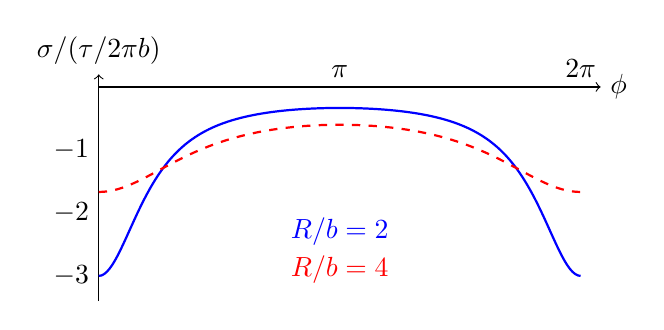
\begin{tikzpicture}[x=.017cm,y=.8cm]
\draw[->] (0,0)--(375,0) node[right] {$\phi$};
\draw[->] (0,-3.4)--(0,.2) node[above] {$\sigma/(\tau/2\pi b)$};
\draw[blue,thick,domain=0:360,samples=180] plot (\x,{-3/(5-4*cos(\x))});
\draw[red,dashed,thick,domain=0:360,samples=180] plot (\x,{-15/(17-8*cos(\x))});
\node[above] at (180,0) {$\pi$};\node[above] at (360,0) {$2\pi$};
\foreach \y in {-1,-2,-3} \node[left] at (0,\y) {$\y$};
\node[blue] at (180,-2.3) {$R/b=2$};
\node[red] at (180,-2.9) {$R/b=4$};
\end{tikzpicture}
\end{center}
\textbf{(d)} The image field at the real line is
$-\tau\widehat{\mathbf x}/[2\pi\epsilon _0(R-c)]$. Thus
\[
\boxed{\frac{\mathbf F}{L}
=-\frac{\tau^2R}{2\pi\epsilon _0(R^2-b^2)}\widehat{\mathbf x},}
\]
an attraction for either sign of $\tau$.

\Needspace{5\baselineskip}
\par\bigskip
\noindent\textbf{2.12}\quad Starting with the series solution (2.71) for the two-dimensional potential problem with the potential specified on the surface of a cylinder of radius $b$, evaluate the coefficients formally, substitute them into the series, and sum it to obtain the potential \emph{inside} the cylinder in the form of Poisson's integral:
\[
\Phi(\rho,\phi)=\frac{1}{2\pi}\int_{0}^{2\pi}\Phi(b,\phi')\,\frac{b^{2}-\rho^{2}}{b^{2}+\rho^{2}-2b\rho\cos(\phi'-\phi)}\;d\phi'
\]
What modification is necessary if the potential is desired in the region of space bounded by the cylinder and infinity?
\solution
Write $f(\phi)=\Phi(b,\phi)$. The nonsingular interior specialization
of (2.71) is
\[
\Phi=A_0+\sum_{n=1}^\infty\left(\frac\rho b\right)^n
 [A_n\cos n\phi+B_n\sin n\phi].
\]
Orthogonality over $[0,2\pi]$ determines
\[
A_0=\frac1{2\pi}\int_0^{2\pi}f(\phi')\,d\phi',\quad
A_n=\frac1\pi\int_0^{2\pi}f(\phi')\cos n\phi'\,d\phi',\quad
B_n=\frac1\pi\int_0^{2\pi}f(\phi')\sin n\phi'\,d\phi'.
\]
Substitution and the cosine subtraction identity give, with $t=\rho/b<1$,
\[
\Phi=\frac1{2\pi}\int_0^{2\pi}f(\phi')
 \left[1+2\sum_{n=1}^\infty t^n\cos n(\phi-\phi')\right]d\phi'.
\]
The series is absolutely convergent inside the circle. Summing the
two geometric series explicitly,
\[
1+\frac{te^{i\Delta}}{1-te^{i\Delta}}
  +\frac{te^{-i\Delta}}{1-te^{-i\Delta}}
=\frac{1-t^2}{1-2t\cos\Delta+t^2}.
\]
Therefore
\[
\boxed{\Phi(\rho,\phi)=\frac1{2\pi}\int_0^{2\pi}f(\phi')
 \frac{b^2-\rho^2}{b^2+\rho^2-2b\rho\cos(\phi-\phi')}\,d\phi'.}
\]
For a solution bounded at infinity replace every $(\rho/b)^n$ by
$(b/\rho)^n$. Equivalently the exterior kernel has numerator
$\rho^2-b^2$ and the same denominator. Its limit at infinity is the
boundary average $A_0$; a zero potential at infinity is possible
with a bounded solution only if $A_0=0$. If logarithmic growth is
allowed, add $B_0\ln(\rho/b)$, which vanishes on the cylinder but
corresponds to a net line charge. The boundary values alone do not
fix $B_0$ without an exterior condition.

\Needspace{5\baselineskip}
\par\bigskip
\noindent\textbf{2.13}\quad\begin{enumerate}
\item[(a)] Two halves of a long hollow conducting cylinder of inner radius $b$ are separated by small lengthwise gaps on each side, and are kept at different potentials $V_{1}$ and $V_{2}$. Show that the potential inside is given by
\[
\Phi(\rho,\phi)=\frac{V_{1}+V_{2}}{2}+\frac{V_{1}-V_{2}}{\pi}\tan^{-1}\!\left(\frac{2b\rho}{b^{2}-\rho^{2}}\cos\phi\right)
\]
where $\phi$ is measured from a plane perpendicular to the plane through the gap.
\item[(b)] Calculate the surface-charge density on each half of the cylinder.
\end{enumerate}
\solution
Choose the $V_1$ half to be $\cos\phi>0$, and the $V_2$ half to be
$\cos\phi<0$. Define $\overline V=(V_1+V_2)/2$ and
$\Delta V=V_1-V_2$.
\textbf{(a)} The boundary function is
$f(\phi)=\overline V+(\Delta V/2)\operatorname{sgn}(\cos\phi)$.
Its sine coefficients vanish. Its cosine coefficients are zero for
even $n$, and for $n=2j+1$ are
\[
A_{2j+1}=\frac{\Delta V}{\pi}\int_{-\pi/2}^{\pi/2}
       \cos[(2j+1)\phi]\,d\phi
=\frac{2\Delta V}{\pi}\frac{(-1)^j}{2j+1}.
\]
Thus, for $t=\rho/b<1$,
\[
\Phi-\overline V=\frac{2\Delta V}{\pi}
 \operatorname{Re}\sum_{j=0}^\infty
       \frac{(-1)^j(te^{i\phi})^{2j+1}}{2j+1}
=\frac{2\Delta V}{\pi}\operatorname{Re}\tan^{-1}(te^{i\phi}).
\]
From $\tan^{-1}w=(2i)^{-1}\ln[(1+iw)/(1-iw)]$, or the tangent
addition formula applied to $w,\bar w$, one obtains
\[
2\operatorname{Re}\tan^{-1}(te^{i\phi})
=\tan^{-1}\frac{2t\cos\phi}{1-t^2}.
\]
Both sides vanish at $t=0$ and remain on the same continuous branch
for $t<1$. Consequently
\[
\boxed{\Phi=\overline V+\frac{\Delta V}{\pi}
 \tan^{-1}\frac{2b\rho\cos\phi}{b^2-\rho^2}.}
\]
As $\rho\uparrow b$ the inverse tangent tends to
$(\pi/2)\operatorname{sgn}(\cos\phi)$, as required.
\textbf{(b)} The normal from the conductor into the cavity is
$-\widehat{\boldsymbol\rho}$, so $\sigma_{\rm inner}=\epsilon _0
\partial_\rho\Phi|_{b^-}$. In terms of $t$ the derivative is
\[
\partial_\rho\Phi=\frac{\Delta V}{\pi b}
 \frac{2(1+t^2)\cos\phi}{(1-t^2)^2+4t^2\cos^2\phi}.
\]
Taking $t\to1$ away from the gaps gives
\[
\boxed{\sigma_{\rm inner}(\phi)=
       \frac{\epsilon _0(V_1-V_2)}{\pi b\cos\phi}.}
\]
For $V_1>V_2$ this is positive on the $V_1$ half and negative on the
$V_2$ half. It diverges as inverse distance to an ideal zero-width
gap; a finite gap cuts off the logarithmic divergence of the charge
on either half. The data for the cavity do not determine the charge
on the exterior faces without exterior geometry and boundary data.

\Needspace{5\baselineskip}
\par\bigskip
\noindent\textbf{2.14}\quad A variant of the preceding two-dimensional problem is a long hollow conducting cylinder of radius $b$ that is divided into equal quarters, alternate segments being held at potential $+V$ and $-V$.
\begin{enumerate}
\item[(a)] Solve by means of the series solution (2.71) and show that the potential inside the cylinder is
\[
\Phi(\rho,\phi)=\frac{4V}{\pi}\sum_{n=0}^{\infty}\left(\frac{\rho}{b}\right)^{4n+2}\frac{\sin[(4n+2)\phi]}{2n+1}
\]
\item[(b)] Sum the series and show that
\[
\Phi(\rho,\phi)=\frac{2V}{\pi}\tan^{-1}\!\left(\frac{2\rho^{2}b^{2}\sin2\phi}{b^{4}-\rho^{4}}\right)
\]
\item[(c)] Sketch the field lines and equipotentials.
\end{enumerate}
\solution
Let the sectors $0<\phi<\pi/2$ and $\pi<\phi<3\pi/2$ be at $+V$;
the other two are at $-V$.
\textbf{(a)} The boundary function is $V\operatorname{sgn}(\sin2\phi)$.
It is odd in $\phi$, invariant under $\phi\mapsto\phi+\pi$, and
changes sign under $\phi\mapsto\phi+\pi/2$. These symmetries leave
only sine modes with $m=4n+2$. Direct integration gives
\[
B_m=\frac1\pi\int_0^{2\pi}V\operatorname{sgn}(\sin2\phi)
                                  \sin m\phi\,d\phi
=\frac{8V}{\pi m},\quad m=4n+2.
\]
The regular radial solution for mode $m$ is $(\rho/b)^m$, whence
\[
\boxed{\Phi=\frac{4V}{\pi}\sum_{n=0}^\infty
 \frac{(\rho/b)^{4n+2}\sin[(4n+2)\phi]}{2n+1}.}
\]
\textbf{(b)} Put $\zeta=(x+iy)/b$. The elementary identity
$\operatorname{artanh}w=\sum_{n\geq0}w^{2n+1}/(2n+1)
=\tfrac12\ln[(1+w)/(1-w)]$ gives
\[
\Phi=\frac{4V}{\pi}\operatorname{Im}\operatorname{artanh}(\zeta^2)
=\frac{2V}{\pi}\arg\frac{1+\zeta^2}{1-\zeta^2}.
\]
Multiplication by $1-\bar\zeta^2$ makes the real and imaginary
parts of this quotient proportional to
$1-|\zeta|^4$ and $2\operatorname{Im}\zeta^2$. The real part is
positive for $|\zeta|<1$, fixing the inverse tangent branch. Hence
\[
\boxed{\Phi=\frac{2V}{\pi}\tan^{-1}
 \frac{2\rho^2b^2\sin2\phi}{b^4-\rho^4}.}
\]
\textbf{(c)} An exact description of the two orthogonal curve families
is obtained by writing
$\operatorname{artanh}\zeta^2=u+iv$. Equipotentials have
$v=\pi\Phi/(4V)$ constant; field lines have $u$ constant, with
arrows toward decreasing $v$. In Cartesian form these conditions are
\[
\frac{4b^2xy}{b^4-(x^2+y^2)^2}
 =\tan\frac{\pi\Phi}{2V},\qquad
\left|\frac{1+\zeta^2}{1-\zeta^2}\right|=e^{2u},
\]
respectively. The supplementary plot is generated parametrically by
$\zeta=\pm\sqrt{\tanh(u+iv)}$, so its curves follow the summed
solution rather than a truncated Fourier series.
\begin{center}
% Generated by supplementary/check_ch02.py --write-assets
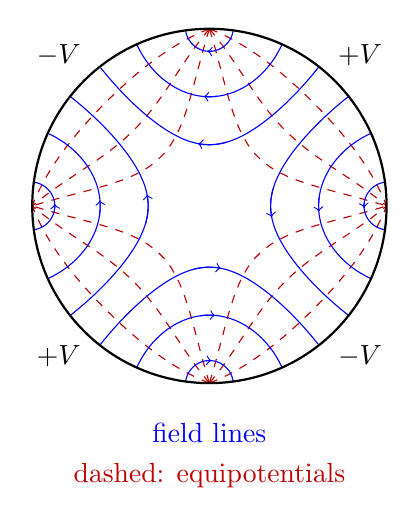
\begin{tikzpicture}[scale=2.25]
\draw[red!75!black,dashed,thin] plot coordinates {(-0.000850,0.999669) (-0.000933,0.999637) (-0.001025,0.999601) (-0.001126,0.999561) (-0.001237,0.999518) (-0.001359,0.999471) (-0.001493,0.999418) (-0.001640,0.999361) (-0.001801,0.999298) (-0.001978,0.999229) (-0.002173,0.999152) (-0.002387,0.999069) (-0.002622,0.998977) (-0.002880,0.998876) (-0.003163,0.998764) (-0.003474,0.998642) (-0.003816,0.998508) (-0.004191,0.998360) (-0.004604,0.998198) (-0.005056,0.998020) (-0.005553,0.997823) (-0.006099,0.997607) (-0.006698,0.997370) (-0.007356,0.997109) (-0.008079,0.996822) (-0.008872,0.996506) (-0.009742,0.996158) (-0.010698,0.995775) (-0.011747,0.995354) (-0.012898,0.994890) (-0.014162,0.994379) (-0.015548,0.993816) (-0.017070,0.993196) (-0.018739,0.992513) (-0.020569,0.991760) (-0.022577,0.990929) (-0.024779,0.990013) (-0.027192,0.989003) (-0.029838,0.987887) (-0.032738,0.986655) (-0.035915,0.985295) (-0.039394,0.983791) (-0.043204,0.982129) (-0.047375,0.980290) (-0.051938,0.978255) (-0.056928,0.976002) (-0.062383,0.973507) (-0.068343,0.970742) (-0.074850,0.967676) (-0.081950,0.964275) (-0.089691,0.960501) (-0.098123,0.956312) (-0.107300,0.951660) (-0.117276,0.946494) (-0.128107,0.940756) (-0.139852,0.934382) (-0.152567,0.927304) (-0.166310,0.919447) (-0.181134,0.910732) (-0.197090,0.901073) (-0.214225,0.890382) (-0.232576,0.878569) (-0.252172,0.865543) (-0.273028,0.851216) (-0.295147,0.835507) (-0.318509,0.818347) (-0.343080,0.799683) (-0.368796,0.779484) (-0.395571,0.757749) (-0.423291,0.734508) (-0.451812,0.709832) (-0.480961,0.683830) (-0.510541,0.656653) (-0.540327,0.628487) (-0.570080,0.599550) (-0.599550,0.570080) (-0.628487,0.540327) (-0.656653,0.510541) (-0.683830,0.480961) (-0.709832,0.451812) (-0.734508,0.423291) (-0.757749,0.395571) (-0.779484,0.368796) (-0.799683,0.343080) (-0.818347,0.318509) (-0.835507,0.295147) (-0.851216,0.273028) (-0.865543,0.252172) (-0.878569,0.232576) (-0.890382,0.214225) (-0.901073,0.197090) (-0.910732,0.181134) (-0.919447,0.166310) (-0.927304,0.152567) (-0.934382,0.139852) (-0.940756,0.128107) (-0.946494,0.117276) (-0.951660,0.107300) (-0.956312,0.098123) (-0.960501,0.089691) (-0.964275,0.081950) (-0.967676,0.074850) (-0.970742,0.068343) (-0.973507,0.062383) (-0.976002,0.056928) (-0.978255,0.051938) (-0.980290,0.047375) (-0.982129,0.043204) (-0.983791,0.039394) (-0.985295,0.035915) (-0.986655,0.032738) (-0.987887,0.029838) (-0.989003,0.027192) (-0.990013,0.024779) (-0.990929,0.022577) (-0.991760,0.020569) (-0.992513,0.018739) (-0.993196,0.017070) (-0.993816,0.015548) (-0.994379,0.014162) (-0.994890,0.012898) (-0.995354,0.011747) (-0.995775,0.010698) (-0.996158,0.009742) (-0.996506,0.008872) (-0.996822,0.008079) (-0.997109,0.007356) (-0.997370,0.006698) (-0.997607,0.006099) (-0.997823,0.005553) (-0.998020,0.005056) (-0.998198,0.004604) (-0.998360,0.004191) (-0.998508,0.003816) (-0.998642,0.003474) (-0.998764,0.003163) (-0.998876,0.002880) (-0.998977,0.002622) (-0.999069,0.002387) (-0.999152,0.002173) (-0.999229,0.001978) (-0.999298,0.001801) (-0.999361,0.001640) (-0.999418,0.001493) (-0.999471,0.001359) (-0.999518,0.001237) (-0.999561,0.001126) (-0.999601,0.001025) (-0.999637,0.000933) (-0.999669,0.000850)};
\draw[red!75!black,dashed,thin] plot coordinates {(0.000850,-0.999669) (0.000933,-0.999637) (0.001025,-0.999601) (0.001126,-0.999561) (0.001237,-0.999518) (0.001359,-0.999471) (0.001493,-0.999418) (0.001640,-0.999361) (0.001801,-0.999298) (0.001978,-0.999229) (0.002173,-0.999152) (0.002387,-0.999069) (0.002622,-0.998977) (0.002880,-0.998876) (0.003163,-0.998764) (0.003474,-0.998642) (0.003816,-0.998508) (0.004191,-0.998360) (0.004604,-0.998198) (0.005056,-0.998020) (0.005553,-0.997823) (0.006099,-0.997607) (0.006698,-0.997370) (0.007356,-0.997109) (0.008079,-0.996822) (0.008872,-0.996506) (0.009742,-0.996158) (0.010698,-0.995775) (0.011747,-0.995354) (0.012898,-0.994890) (0.014162,-0.994379) (0.015548,-0.993816) (0.017070,-0.993196) (0.018739,-0.992513) (0.020569,-0.991760) (0.022577,-0.990929) (0.024779,-0.990013) (0.027192,-0.989003) (0.029838,-0.987887) (0.032738,-0.986655) (0.035915,-0.985295) (0.039394,-0.983791) (0.043204,-0.982129) (0.047375,-0.980290) (0.051938,-0.978255) (0.056928,-0.976002) (0.062383,-0.973507) (0.068343,-0.970742) (0.074850,-0.967676) (0.081950,-0.964275) (0.089691,-0.960501) (0.098123,-0.956312) (0.107300,-0.951660) (0.117276,-0.946494) (0.128107,-0.940756) (0.139852,-0.934382) (0.152567,-0.927304) (0.166310,-0.919447) (0.181134,-0.910732) (0.197090,-0.901073) (0.214225,-0.890382) (0.232576,-0.878569) (0.252172,-0.865543) (0.273028,-0.851216) (0.295147,-0.835507) (0.318509,-0.818347) (0.343080,-0.799683) (0.368796,-0.779484) (0.395571,-0.757749) (0.423291,-0.734508) (0.451812,-0.709832) (0.480961,-0.683830) (0.510541,-0.656653) (0.540327,-0.628487) (0.570080,-0.599550) (0.599550,-0.570080) (0.628487,-0.540327) (0.656653,-0.510541) (0.683830,-0.480961) (0.709832,-0.451812) (0.734508,-0.423291) (0.757749,-0.395571) (0.779484,-0.368796) (0.799683,-0.343080) (0.818347,-0.318509) (0.835507,-0.295147) (0.851216,-0.273028) (0.865543,-0.252172) (0.878569,-0.232576) (0.890382,-0.214225) (0.901073,-0.197090) (0.910732,-0.181134) (0.919447,-0.166310) (0.927304,-0.152567) (0.934382,-0.139852) (0.940756,-0.128107) (0.946494,-0.117276) (0.951660,-0.107300) (0.956312,-0.098123) (0.960501,-0.089691) (0.964275,-0.081950) (0.967676,-0.074850) (0.970742,-0.068343) (0.973507,-0.062383) (0.976002,-0.056928) (0.978255,-0.051938) (0.980290,-0.047375) (0.982129,-0.043204) (0.983791,-0.039394) (0.985295,-0.035915) (0.986655,-0.032738) (0.987887,-0.029838) (0.989003,-0.027192) (0.990013,-0.024779) (0.990929,-0.022577) (0.991760,-0.020569) (0.992513,-0.018739) (0.993196,-0.017070) (0.993816,-0.015548) (0.994379,-0.014162) (0.994890,-0.012898) (0.995354,-0.011747) (0.995775,-0.010698) (0.996158,-0.009742) (0.996506,-0.008872) (0.996822,-0.008079) (0.997109,-0.007356) (0.997370,-0.006698) (0.997607,-0.006099) (0.997823,-0.005553) (0.998020,-0.005056) (0.998198,-0.004604) (0.998360,-0.004191) (0.998508,-0.003816) (0.998642,-0.003474) (0.998764,-0.003163) (0.998876,-0.002880) (0.998977,-0.002622) (0.999069,-0.002387) (0.999152,-0.002173) (0.999229,-0.001978) (0.999298,-0.001801) (0.999361,-0.001640) (0.999418,-0.001493) (0.999471,-0.001359) (0.999518,-0.001237) (0.999561,-0.001126) (0.999601,-0.001025) (0.999637,-0.000933) (0.999669,-0.000850)};
\draw[red!75!black,dashed,thin] plot coordinates {(-0.000587,0.999303) (-0.000645,0.999234) (-0.000708,0.999158) (-0.000778,0.999076) (-0.000855,0.998985) (-0.000939,0.998884) (-0.001031,0.998775) (-0.001132,0.998654) (-0.001244,0.998521) (-0.001366,0.998376) (-0.001501,0.998216) (-0.001648,0.998040) (-0.001810,0.997847) (-0.001988,0.997635) (-0.002183,0.997402) (-0.002398,0.997146) (-0.002633,0.996865) (-0.002892,0.996557) (-0.003176,0.996217) (-0.003487,0.995845) (-0.003829,0.995436) (-0.004205,0.994987) (-0.004617,0.994493) (-0.005069,0.993951) (-0.005565,0.993356) (-0.006109,0.992702) (-0.006706,0.991984) (-0.007361,0.991196) (-0.008079,0.990329) (-0.008867,0.989378) (-0.009730,0.988334) (-0.010677,0.987187) (-0.011714,0.985928) (-0.012850,0.984545) (-0.014095,0.983026) (-0.015459,0.981359) (-0.016951,0.979529) (-0.018584,0.977520) (-0.020371,0.975315) (-0.022325,0.972895) (-0.024462,0.970238) (-0.026796,0.967323) (-0.029345,0.964125) (-0.032127,0.960617) (-0.035162,0.956769) (-0.038471,0.952549) (-0.042075,0.947923) (-0.045999,0.942852) (-0.050268,0.937295) (-0.054907,0.931209) (-0.059944,0.924544) (-0.065409,0.917249) (-0.071332,0.909268) (-0.077743,0.900541) (-0.084677,0.891006) (-0.092167,0.880595) (-0.100249,0.869236) (-0.108959,0.856856) (-0.118337,0.843376) (-0.128424,0.828717) (-0.139262,0.812800) (-0.150901,0.795545) (-0.163392,0.776873) (-0.176796,0.756715) (-0.191180,0.735008) (-0.206625,0.711704) (-0.223225,0.686778) (-0.241091,0.660237) (-0.260350,0.632132) (-0.281142,0.602573) (-0.303613,0.571748) (-0.327888,0.539942) (-0.354045,0.507541) (-0.382066,0.475026) (-0.411799,0.442935) (-0.442935,0.411799) (-0.475026,0.382066) (-0.507541,0.354045) (-0.539942,0.327888) (-0.571748,0.303613) (-0.602573,0.281142) (-0.632132,0.260350) (-0.660237,0.241091) (-0.686778,0.223225) (-0.711704,0.206625) (-0.735008,0.191180) (-0.756715,0.176796) (-0.776873,0.163392) (-0.795545,0.150901) (-0.812800,0.139262) (-0.828717,0.128424) (-0.843376,0.118337) (-0.856856,0.108959) (-0.869236,0.100249) (-0.880595,0.092167) (-0.891006,0.084677) (-0.900541,0.077743) (-0.909268,0.071332) (-0.917249,0.065409) (-0.924544,0.059944) (-0.931209,0.054907) (-0.937295,0.050268) (-0.942852,0.045999) (-0.947923,0.042075) (-0.952549,0.038471) (-0.956769,0.035162) (-0.960617,0.032127) (-0.964125,0.029345) (-0.967323,0.026796) (-0.970238,0.024462) (-0.972895,0.022325) (-0.975315,0.020371) (-0.977520,0.018584) (-0.979529,0.016951) (-0.981359,0.015459) (-0.983026,0.014095) (-0.984545,0.012850) (-0.985928,0.011714) (-0.987187,0.010677) (-0.988334,0.009730) (-0.989378,0.008867) (-0.990329,0.008079) (-0.991196,0.007361) (-0.991984,0.006706) (-0.992702,0.006109) (-0.993356,0.005565) (-0.993951,0.005069) (-0.994493,0.004617) (-0.994987,0.004205) (-0.995436,0.003829) (-0.995845,0.003487) (-0.996217,0.003176) (-0.996557,0.002892) (-0.996865,0.002633) (-0.997146,0.002398) (-0.997402,0.002183) (-0.997635,0.001988) (-0.997847,0.001810) (-0.998040,0.001648) (-0.998216,0.001501) (-0.998376,0.001366) (-0.998521,0.001244) (-0.998654,0.001132) (-0.998775,0.001031) (-0.998884,0.000939) (-0.998985,0.000855) (-0.999076,0.000778) (-0.999158,0.000708) (-0.999234,0.000645) (-0.999303,0.000587)};
\draw[red!75!black,dashed,thin] plot coordinates {(0.000587,-0.999303) (0.000645,-0.999234) (0.000708,-0.999158) (0.000778,-0.999076) (0.000855,-0.998985) (0.000939,-0.998884) (0.001031,-0.998775) (0.001132,-0.998654) (0.001244,-0.998521) (0.001366,-0.998376) (0.001501,-0.998216) (0.001648,-0.998040) (0.001810,-0.997847) (0.001988,-0.997635) (0.002183,-0.997402) (0.002398,-0.997146) (0.002633,-0.996865) (0.002892,-0.996557) (0.003176,-0.996217) (0.003487,-0.995845) (0.003829,-0.995436) (0.004205,-0.994987) (0.004617,-0.994493) (0.005069,-0.993951) (0.005565,-0.993356) (0.006109,-0.992702) (0.006706,-0.991984) (0.007361,-0.991196) (0.008079,-0.990329) (0.008867,-0.989378) (0.009730,-0.988334) (0.010677,-0.987187) (0.011714,-0.985928) (0.012850,-0.984545) (0.014095,-0.983026) (0.015459,-0.981359) (0.016951,-0.979529) (0.018584,-0.977520) (0.020371,-0.975315) (0.022325,-0.972895) (0.024462,-0.970238) (0.026796,-0.967323) (0.029345,-0.964125) (0.032127,-0.960617) (0.035162,-0.956769) (0.038471,-0.952549) (0.042075,-0.947923) (0.045999,-0.942852) (0.050268,-0.937295) (0.054907,-0.931209) (0.059944,-0.924544) (0.065409,-0.917249) (0.071332,-0.909268) (0.077743,-0.900541) (0.084677,-0.891006) (0.092167,-0.880595) (0.100249,-0.869236) (0.108959,-0.856856) (0.118337,-0.843376) (0.128424,-0.828717) (0.139262,-0.812800) (0.150901,-0.795545) (0.163392,-0.776873) (0.176796,-0.756715) (0.191180,-0.735008) (0.206625,-0.711704) (0.223225,-0.686778) (0.241091,-0.660237) (0.260350,-0.632132) (0.281142,-0.602573) (0.303613,-0.571748) (0.327888,-0.539942) (0.354045,-0.507541) (0.382066,-0.475026) (0.411799,-0.442935) (0.442935,-0.411799) (0.475026,-0.382066) (0.507541,-0.354045) (0.539942,-0.327888) (0.571748,-0.303613) (0.602573,-0.281142) (0.632132,-0.260350) (0.660237,-0.241091) (0.686778,-0.223225) (0.711704,-0.206625) (0.735008,-0.191180) (0.756715,-0.176796) (0.776873,-0.163392) (0.795545,-0.150901) (0.812800,-0.139262) (0.828717,-0.128424) (0.843376,-0.118337) (0.856856,-0.108959) (0.869236,-0.100249) (0.880595,-0.092167) (0.891006,-0.084677) (0.900541,-0.077743) (0.909268,-0.071332) (0.917249,-0.065409) (0.924544,-0.059944) (0.931209,-0.054907) (0.937295,-0.050268) (0.942852,-0.045999) (0.947923,-0.042075) (0.952549,-0.038471) (0.956769,-0.035162) (0.960617,-0.032127) (0.964125,-0.029345) (0.967323,-0.026796) (0.970238,-0.024462) (0.972895,-0.022325) (0.975315,-0.020371) (0.977520,-0.018584) (0.979529,-0.016951) (0.981359,-0.015459) (0.983026,-0.014095) (0.984545,-0.012850) (0.985928,-0.011714) (0.987187,-0.010677) (0.988334,-0.009730) (0.989378,-0.008867) (0.990329,-0.008079) (0.991196,-0.007361) (0.991984,-0.006706) (0.992702,-0.006109) (0.993356,-0.005565) (0.993951,-0.005069) (0.994493,-0.004617) (0.994987,-0.004205) (0.995436,-0.003829) (0.995845,-0.003487) (0.996217,-0.003176) (0.996557,-0.002892) (0.996865,-0.002633) (0.997146,-0.002398) (0.997402,-0.002183) (0.997635,-0.001988) (0.997847,-0.001810) (0.998040,-0.001648) (0.998216,-0.001501) (0.998376,-0.001366) (0.998521,-0.001244) (0.998654,-0.001132) (0.998775,-0.001031) (0.998884,-0.000939) (0.998985,-0.000855) (0.999076,-0.000778) (0.999158,-0.000708) (0.999234,-0.000645) (0.999303,-0.000587)};
\draw[red!75!black,dashed,thin] plot coordinates {(-0.000269,0.999129) (-0.000296,0.999043) (-0.000325,0.998949) (-0.000357,0.998846) (-0.000392,0.998732) (-0.000430,0.998607) (-0.000473,0.998470) (-0.000519,0.998320) (-0.000570,0.998154) (-0.000626,0.997973) (-0.000688,0.997773) (-0.000756,0.997554) (-0.000830,0.997313) (-0.000911,0.997049) (-0.001001,0.996759) (-0.001099,0.996440) (-0.001207,0.996090) (-0.001325,0.995705) (-0.001455,0.995283) (-0.001598,0.994819) (-0.001755,0.994310) (-0.001926,0.993751) (-0.002115,0.993137) (-0.002322,0.992464) (-0.002549,0.991724) (-0.002797,0.990912) (-0.003070,0.990021) (-0.003369,0.989042) (-0.003697,0.987969) (-0.004057,0.986791) (-0.004451,0.985498) (-0.004883,0.984079) (-0.005356,0.982523) (-0.005873,0.980816) (-0.006440,0.978944) (-0.007060,0.976891) (-0.007739,0.974640) (-0.008481,0.972172) (-0.009292,0.969468) (-0.010178,0.966505) (-0.011146,0.963258) (-0.012202,0.959703) (-0.013355,0.955810) (-0.014611,0.951549) (-0.015980,0.946886) (-0.017471,0.941786) (-0.019092,0.936209) (-0.020855,0.930113) (-0.022770,0.923454) (-0.024849,0.916182) (-0.027103,0.908245) (-0.029546,0.899587) (-0.032190,0.890147) (-0.035050,0.879862) (-0.038141,0.868662) (-0.041479,0.856473) (-0.045082,0.843218) (-0.048970,0.828813) (-0.053163,0.813169) (-0.057687,0.796190) (-0.062572,0.777774) (-0.067852,0.757812) (-0.073572,0.736186) (-0.079789,0.712766) (-0.086577,0.687413) (-0.094036,0.659970) (-0.102305,0.630266) (-0.111579,0.598109) (-0.122138,0.563290) (-0.134392,0.525592) (-0.148956,0.484820) (-0.166743,0.440895) (-0.189079,0.394077) (-0.217653,0.345435) (-0.253896,0.297464) (-0.297464,0.253896) (-0.345435,0.217653) (-0.394077,0.189079) (-0.440895,0.166743) (-0.484820,0.148956) (-0.525592,0.134392) (-0.563290,0.122138) (-0.598109,0.111579) (-0.630266,0.102305) (-0.659970,0.094036) (-0.687413,0.086577) (-0.712766,0.079789) (-0.736186,0.073572) (-0.757812,0.067852) (-0.777774,0.062572) (-0.796190,0.057687) (-0.813169,0.053163) (-0.828813,0.048970) (-0.843218,0.045082) (-0.856473,0.041479) (-0.868662,0.038141) (-0.879862,0.035050) (-0.890147,0.032190) (-0.899587,0.029546) (-0.908245,0.027103) (-0.916182,0.024849) (-0.923454,0.022770) (-0.930113,0.020855) (-0.936209,0.019092) (-0.941786,0.017471) (-0.946886,0.015980) (-0.951549,0.014611) (-0.955810,0.013355) (-0.959703,0.012202) (-0.963258,0.011146) (-0.966505,0.010178) (-0.969468,0.009292) (-0.972172,0.008481) (-0.974640,0.007739) (-0.976891,0.007060) (-0.978944,0.006440) (-0.980816,0.005873) (-0.982523,0.005356) (-0.984079,0.004883) (-0.985498,0.004451) (-0.986791,0.004057) (-0.987969,0.003697) (-0.989042,0.003369) (-0.990021,0.003070) (-0.990912,0.002797) (-0.991724,0.002549) (-0.992464,0.002322) (-0.993137,0.002115) (-0.993751,0.001926) (-0.994310,0.001755) (-0.994819,0.001598) (-0.995283,0.001455) (-0.995705,0.001325) (-0.996090,0.001207) (-0.996440,0.001099) (-0.996759,0.001001) (-0.997049,0.000911) (-0.997313,0.000830) (-0.997554,0.000756) (-0.997773,0.000688) (-0.997973,0.000626) (-0.998154,0.000570) (-0.998320,0.000519) (-0.998470,0.000473) (-0.998607,0.000430) (-0.998732,0.000392) (-0.998846,0.000357) (-0.998949,0.000325) (-0.999043,0.000296) (-0.999129,0.000269)};
\draw[red!75!black,dashed,thin] plot coordinates {(0.000269,-0.999129) (0.000296,-0.999043) (0.000325,-0.998949) (0.000357,-0.998846) (0.000392,-0.998732) (0.000430,-0.998607) (0.000473,-0.998470) (0.000519,-0.998320) (0.000570,-0.998154) (0.000626,-0.997973) (0.000688,-0.997773) (0.000756,-0.997554) (0.000830,-0.997313) (0.000911,-0.997049) (0.001001,-0.996759) (0.001099,-0.996440) (0.001207,-0.996090) (0.001325,-0.995705) (0.001455,-0.995283) (0.001598,-0.994819) (0.001755,-0.994310) (0.001926,-0.993751) (0.002115,-0.993137) (0.002322,-0.992464) (0.002549,-0.991724) (0.002797,-0.990912) (0.003070,-0.990021) (0.003369,-0.989042) (0.003697,-0.987969) (0.004057,-0.986791) (0.004451,-0.985498) (0.004883,-0.984079) (0.005356,-0.982523) (0.005873,-0.980816) (0.006440,-0.978944) (0.007060,-0.976891) (0.007739,-0.974640) (0.008481,-0.972172) (0.009292,-0.969468) (0.010178,-0.966505) (0.011146,-0.963258) (0.012202,-0.959703) (0.013355,-0.955810) (0.014611,-0.951549) (0.015980,-0.946886) (0.017471,-0.941786) (0.019092,-0.936209) (0.020855,-0.930113) (0.022770,-0.923454) (0.024849,-0.916182) (0.027103,-0.908245) (0.029546,-0.899587) (0.032190,-0.890147) (0.035050,-0.879862) (0.038141,-0.868662) (0.041479,-0.856473) (0.045082,-0.843218) (0.048970,-0.828813) (0.053163,-0.813169) (0.057687,-0.796190) (0.062572,-0.777774) (0.067852,-0.757812) (0.073572,-0.736186) (0.079789,-0.712766) (0.086577,-0.687413) (0.094036,-0.659970) (0.102305,-0.630266) (0.111579,-0.598109) (0.122138,-0.563290) (0.134392,-0.525592) (0.148956,-0.484820) (0.166743,-0.440895) (0.189079,-0.394077) (0.217653,-0.345435) (0.253896,-0.297464) (0.297464,-0.253896) (0.345435,-0.217653) (0.394077,-0.189079) (0.440895,-0.166743) (0.484820,-0.148956) (0.525592,-0.134392) (0.563290,-0.122138) (0.598109,-0.111579) (0.630266,-0.102305) (0.659970,-0.094036) (0.687413,-0.086577) (0.712766,-0.079789) (0.736186,-0.073572) (0.757812,-0.067852) (0.777774,-0.062572) (0.796190,-0.057687) (0.813169,-0.053163) (0.828813,-0.048970) (0.843218,-0.045082) (0.856473,-0.041479) (0.868662,-0.038141) (0.879862,-0.035050) (0.890147,-0.032190) (0.899587,-0.029546) (0.908245,-0.027103) (0.916182,-0.024849) (0.923454,-0.022770) (0.930113,-0.020855) (0.936209,-0.019092) (0.941786,-0.017471) (0.946886,-0.015980) (0.951549,-0.014611) (0.955810,-0.013355) (0.959703,-0.012202) (0.963258,-0.011146) (0.966505,-0.010178) (0.969468,-0.009292) (0.972172,-0.008481) (0.974640,-0.007739) (0.976891,-0.007060) (0.978944,-0.006440) (0.980816,-0.005873) (0.982523,-0.005356) (0.984079,-0.004883) (0.985498,-0.004451) (0.986791,-0.004057) (0.987969,-0.003697) (0.989042,-0.003369) (0.990021,-0.003070) (0.990912,-0.002797) (0.991724,-0.002549) (0.992464,-0.002322) (0.993137,-0.002115) (0.993751,-0.001926) (0.994310,-0.001755) (0.994819,-0.001598) (0.995283,-0.001455) (0.995705,-0.001325) (0.996090,-0.001207) (0.996440,-0.001099) (0.996759,-0.001001) (0.997049,-0.000911) (0.997313,-0.000830) (0.997554,-0.000756) (0.997773,-0.000688) (0.997973,-0.000626) (0.998154,-0.000570) (0.998320,-0.000519) (0.998470,-0.000473) (0.998607,-0.000430) (0.998732,-0.000392) (0.998846,-0.000357) (0.998949,-0.000325) (0.999043,-0.000296) (0.999129,-0.000269)};
\draw[red!75!black,dashed,thin] plot coordinates {(-0.000269,-0.999129) (-0.000296,-0.999043) (-0.000325,-0.998949) (-0.000357,-0.998846) (-0.000392,-0.998732) (-0.000430,-0.998607) (-0.000473,-0.998470) (-0.000519,-0.998320) (-0.000570,-0.998154) (-0.000626,-0.997973) (-0.000688,-0.997773) (-0.000756,-0.997554) (-0.000830,-0.997313) (-0.000911,-0.997049) (-0.001001,-0.996759) (-0.001099,-0.996440) (-0.001207,-0.996090) (-0.001325,-0.995705) (-0.001455,-0.995283) (-0.001598,-0.994819) (-0.001755,-0.994310) (-0.001926,-0.993751) (-0.002115,-0.993137) (-0.002322,-0.992464) (-0.002549,-0.991724) (-0.002797,-0.990912) (-0.003070,-0.990021) (-0.003369,-0.989042) (-0.003697,-0.987969) (-0.004057,-0.986791) (-0.004451,-0.985498) (-0.004883,-0.984079) (-0.005356,-0.982523) (-0.005873,-0.980816) (-0.006440,-0.978944) (-0.007060,-0.976891) (-0.007739,-0.974640) (-0.008481,-0.972172) (-0.009292,-0.969468) (-0.010178,-0.966505) (-0.011146,-0.963258) (-0.012202,-0.959703) (-0.013355,-0.955810) (-0.014611,-0.951549) (-0.015980,-0.946886) (-0.017471,-0.941786) (-0.019092,-0.936209) (-0.020855,-0.930113) (-0.022770,-0.923454) (-0.024849,-0.916182) (-0.027103,-0.908245) (-0.029546,-0.899587) (-0.032190,-0.890147) (-0.035050,-0.879862) (-0.038141,-0.868662) (-0.041479,-0.856473) (-0.045082,-0.843218) (-0.048970,-0.828813) (-0.053163,-0.813169) (-0.057687,-0.796190) (-0.062572,-0.777774) (-0.067852,-0.757812) (-0.073572,-0.736186) (-0.079789,-0.712766) (-0.086577,-0.687413) (-0.094036,-0.659970) (-0.102305,-0.630266) (-0.111579,-0.598109) (-0.122138,-0.563290) (-0.134392,-0.525592) (-0.148956,-0.484820) (-0.166743,-0.440895) (-0.189079,-0.394077) (-0.217653,-0.345435) (-0.253896,-0.297464) (-0.297464,-0.253896) (-0.345435,-0.217653) (-0.394077,-0.189079) (-0.440895,-0.166743) (-0.484820,-0.148956) (-0.525592,-0.134392) (-0.563290,-0.122138) (-0.598109,-0.111579) (-0.630266,-0.102305) (-0.659970,-0.094036) (-0.687413,-0.086577) (-0.712766,-0.079789) (-0.736186,-0.073572) (-0.757812,-0.067852) (-0.777774,-0.062572) (-0.796190,-0.057687) (-0.813169,-0.053163) (-0.828813,-0.048970) (-0.843218,-0.045082) (-0.856473,-0.041479) (-0.868662,-0.038141) (-0.879862,-0.035050) (-0.890147,-0.032190) (-0.899587,-0.029546) (-0.908245,-0.027103) (-0.916182,-0.024849) (-0.923454,-0.022770) (-0.930113,-0.020855) (-0.936209,-0.019092) (-0.941786,-0.017471) (-0.946886,-0.015980) (-0.951549,-0.014611) (-0.955810,-0.013355) (-0.959703,-0.012202) (-0.963258,-0.011146) (-0.966505,-0.010178) (-0.969468,-0.009292) (-0.972172,-0.008481) (-0.974640,-0.007739) (-0.976891,-0.007060) (-0.978944,-0.006440) (-0.980816,-0.005873) (-0.982523,-0.005356) (-0.984079,-0.004883) (-0.985498,-0.004451) (-0.986791,-0.004057) (-0.987969,-0.003697) (-0.989042,-0.003369) (-0.990021,-0.003070) (-0.990912,-0.002797) (-0.991724,-0.002549) (-0.992464,-0.002322) (-0.993137,-0.002115) (-0.993751,-0.001926) (-0.994310,-0.001755) (-0.994819,-0.001598) (-0.995283,-0.001455) (-0.995705,-0.001325) (-0.996090,-0.001207) (-0.996440,-0.001099) (-0.996759,-0.001001) (-0.997049,-0.000911) (-0.997313,-0.000830) (-0.997554,-0.000756) (-0.997773,-0.000688) (-0.997973,-0.000626) (-0.998154,-0.000570) (-0.998320,-0.000519) (-0.998470,-0.000473) (-0.998607,-0.000430) (-0.998732,-0.000392) (-0.998846,-0.000357) (-0.998949,-0.000325) (-0.999043,-0.000296) (-0.999129,-0.000269)};
\draw[red!75!black,dashed,thin] plot coordinates {(0.000269,0.999129) (0.000296,0.999043) (0.000325,0.998949) (0.000357,0.998846) (0.000392,0.998732) (0.000430,0.998607) (0.000473,0.998470) (0.000519,0.998320) (0.000570,0.998154) (0.000626,0.997973) (0.000688,0.997773) (0.000756,0.997554) (0.000830,0.997313) (0.000911,0.997049) (0.001001,0.996759) (0.001099,0.996440) (0.001207,0.996090) (0.001325,0.995705) (0.001455,0.995283) (0.001598,0.994819) (0.001755,0.994310) (0.001926,0.993751) (0.002115,0.993137) (0.002322,0.992464) (0.002549,0.991724) (0.002797,0.990912) (0.003070,0.990021) (0.003369,0.989042) (0.003697,0.987969) (0.004057,0.986791) (0.004451,0.985498) (0.004883,0.984079) (0.005356,0.982523) (0.005873,0.980816) (0.006440,0.978944) (0.007060,0.976891) (0.007739,0.974640) (0.008481,0.972172) (0.009292,0.969468) (0.010178,0.966505) (0.011146,0.963258) (0.012202,0.959703) (0.013355,0.955810) (0.014611,0.951549) (0.015980,0.946886) (0.017471,0.941786) (0.019092,0.936209) (0.020855,0.930113) (0.022770,0.923454) (0.024849,0.916182) (0.027103,0.908245) (0.029546,0.899587) (0.032190,0.890147) (0.035050,0.879862) (0.038141,0.868662) (0.041479,0.856473) (0.045082,0.843218) (0.048970,0.828813) (0.053163,0.813169) (0.057687,0.796190) (0.062572,0.777774) (0.067852,0.757812) (0.073572,0.736186) (0.079789,0.712766) (0.086577,0.687413) (0.094036,0.659970) (0.102305,0.630266) (0.111579,0.598109) (0.122138,0.563290) (0.134392,0.525592) (0.148956,0.484820) (0.166743,0.440895) (0.189079,0.394077) (0.217653,0.345435) (0.253896,0.297464) (0.297464,0.253896) (0.345435,0.217653) (0.394077,0.189079) (0.440895,0.166743) (0.484820,0.148956) (0.525592,0.134392) (0.563290,0.122138) (0.598109,0.111579) (0.630266,0.102305) (0.659970,0.094036) (0.687413,0.086577) (0.712766,0.079789) (0.736186,0.073572) (0.757812,0.067852) (0.777774,0.062572) (0.796190,0.057687) (0.813169,0.053163) (0.828813,0.048970) (0.843218,0.045082) (0.856473,0.041479) (0.868662,0.038141) (0.879862,0.035050) (0.890147,0.032190) (0.899587,0.029546) (0.908245,0.027103) (0.916182,0.024849) (0.923454,0.022770) (0.930113,0.020855) (0.936209,0.019092) (0.941786,0.017471) (0.946886,0.015980) (0.951549,0.014611) (0.955810,0.013355) (0.959703,0.012202) (0.963258,0.011146) (0.966505,0.010178) (0.969468,0.009292) (0.972172,0.008481) (0.974640,0.007739) (0.976891,0.007060) (0.978944,0.006440) (0.980816,0.005873) (0.982523,0.005356) (0.984079,0.004883) (0.985498,0.004451) (0.986791,0.004057) (0.987969,0.003697) (0.989042,0.003369) (0.990021,0.003070) (0.990912,0.002797) (0.991724,0.002549) (0.992464,0.002322) (0.993137,0.002115) (0.993751,0.001926) (0.994310,0.001755) (0.994819,0.001598) (0.995283,0.001455) (0.995705,0.001325) (0.996090,0.001207) (0.996440,0.001099) (0.996759,0.001001) (0.997049,0.000911) (0.997313,0.000830) (0.997554,0.000756) (0.997773,0.000688) (0.997973,0.000626) (0.998154,0.000570) (0.998320,0.000519) (0.998470,0.000473) (0.998607,0.000430) (0.998732,0.000392) (0.998846,0.000357) (0.998949,0.000325) (0.999043,0.000296) (0.999129,0.000269)};
\draw[red!75!black,dashed,thin] plot coordinates {(-0.000587,-0.999303) (-0.000645,-0.999234) (-0.000708,-0.999158) (-0.000778,-0.999076) (-0.000855,-0.998985) (-0.000939,-0.998884) (-0.001031,-0.998775) (-0.001132,-0.998654) (-0.001244,-0.998521) (-0.001366,-0.998376) (-0.001501,-0.998216) (-0.001648,-0.998040) (-0.001810,-0.997847) (-0.001988,-0.997635) (-0.002183,-0.997402) (-0.002398,-0.997146) (-0.002633,-0.996865) (-0.002892,-0.996557) (-0.003176,-0.996217) (-0.003487,-0.995845) (-0.003829,-0.995436) (-0.004205,-0.994987) (-0.004617,-0.994493) (-0.005069,-0.993951) (-0.005565,-0.993356) (-0.006109,-0.992702) (-0.006706,-0.991984) (-0.007361,-0.991196) (-0.008079,-0.990329) (-0.008867,-0.989378) (-0.009730,-0.988334) (-0.010677,-0.987187) (-0.011714,-0.985928) (-0.012850,-0.984545) (-0.014095,-0.983026) (-0.015459,-0.981359) (-0.016951,-0.979529) (-0.018584,-0.977520) (-0.020371,-0.975315) (-0.022325,-0.972895) (-0.024462,-0.970238) (-0.026796,-0.967323) (-0.029345,-0.964125) (-0.032127,-0.960617) (-0.035162,-0.956769) (-0.038471,-0.952549) (-0.042075,-0.947923) (-0.045999,-0.942852) (-0.050268,-0.937295) (-0.054907,-0.931209) (-0.059944,-0.924544) (-0.065409,-0.917249) (-0.071332,-0.909268) (-0.077743,-0.900541) (-0.084677,-0.891006) (-0.092167,-0.880595) (-0.100249,-0.869236) (-0.108959,-0.856856) (-0.118337,-0.843376) (-0.128424,-0.828717) (-0.139262,-0.812800) (-0.150901,-0.795545) (-0.163392,-0.776873) (-0.176796,-0.756715) (-0.191180,-0.735008) (-0.206625,-0.711704) (-0.223225,-0.686778) (-0.241091,-0.660237) (-0.260350,-0.632132) (-0.281142,-0.602573) (-0.303613,-0.571748) (-0.327888,-0.539942) (-0.354045,-0.507541) (-0.382066,-0.475026) (-0.411799,-0.442935) (-0.442935,-0.411799) (-0.475026,-0.382066) (-0.507541,-0.354045) (-0.539942,-0.327888) (-0.571748,-0.303613) (-0.602573,-0.281142) (-0.632132,-0.260350) (-0.660237,-0.241091) (-0.686778,-0.223225) (-0.711704,-0.206625) (-0.735008,-0.191180) (-0.756715,-0.176796) (-0.776873,-0.163392) (-0.795545,-0.150901) (-0.812800,-0.139262) (-0.828717,-0.128424) (-0.843376,-0.118337) (-0.856856,-0.108959) (-0.869236,-0.100249) (-0.880595,-0.092167) (-0.891006,-0.084677) (-0.900541,-0.077743) (-0.909268,-0.071332) (-0.917249,-0.065409) (-0.924544,-0.059944) (-0.931209,-0.054907) (-0.937295,-0.050268) (-0.942852,-0.045999) (-0.947923,-0.042075) (-0.952549,-0.038471) (-0.956769,-0.035162) (-0.960617,-0.032127) (-0.964125,-0.029345) (-0.967323,-0.026796) (-0.970238,-0.024462) (-0.972895,-0.022325) (-0.975315,-0.020371) (-0.977520,-0.018584) (-0.979529,-0.016951) (-0.981359,-0.015459) (-0.983026,-0.014095) (-0.984545,-0.012850) (-0.985928,-0.011714) (-0.987187,-0.010677) (-0.988334,-0.009730) (-0.989378,-0.008867) (-0.990329,-0.008079) (-0.991196,-0.007361) (-0.991984,-0.006706) (-0.992702,-0.006109) (-0.993356,-0.005565) (-0.993951,-0.005069) (-0.994493,-0.004617) (-0.994987,-0.004205) (-0.995436,-0.003829) (-0.995845,-0.003487) (-0.996217,-0.003176) (-0.996557,-0.002892) (-0.996865,-0.002633) (-0.997146,-0.002398) (-0.997402,-0.002183) (-0.997635,-0.001988) (-0.997847,-0.001810) (-0.998040,-0.001648) (-0.998216,-0.001501) (-0.998376,-0.001366) (-0.998521,-0.001244) (-0.998654,-0.001132) (-0.998775,-0.001031) (-0.998884,-0.000939) (-0.998985,-0.000855) (-0.999076,-0.000778) (-0.999158,-0.000708) (-0.999234,-0.000645) (-0.999303,-0.000587)};
\draw[red!75!black,dashed,thin] plot coordinates {(0.000587,0.999303) (0.000645,0.999234) (0.000708,0.999158) (0.000778,0.999076) (0.000855,0.998985) (0.000939,0.998884) (0.001031,0.998775) (0.001132,0.998654) (0.001244,0.998521) (0.001366,0.998376) (0.001501,0.998216) (0.001648,0.998040) (0.001810,0.997847) (0.001988,0.997635) (0.002183,0.997402) (0.002398,0.997146) (0.002633,0.996865) (0.002892,0.996557) (0.003176,0.996217) (0.003487,0.995845) (0.003829,0.995436) (0.004205,0.994987) (0.004617,0.994493) (0.005069,0.993951) (0.005565,0.993356) (0.006109,0.992702) (0.006706,0.991984) (0.007361,0.991196) (0.008079,0.990329) (0.008867,0.989378) (0.009730,0.988334) (0.010677,0.987187) (0.011714,0.985928) (0.012850,0.984545) (0.014095,0.983026) (0.015459,0.981359) (0.016951,0.979529) (0.018584,0.977520) (0.020371,0.975315) (0.022325,0.972895) (0.024462,0.970238) (0.026796,0.967323) (0.029345,0.964125) (0.032127,0.960617) (0.035162,0.956769) (0.038471,0.952549) (0.042075,0.947923) (0.045999,0.942852) (0.050268,0.937295) (0.054907,0.931209) (0.059944,0.924544) (0.065409,0.917249) (0.071332,0.909268) (0.077743,0.900541) (0.084677,0.891006) (0.092167,0.880595) (0.100249,0.869236) (0.108959,0.856856) (0.118337,0.843376) (0.128424,0.828717) (0.139262,0.812800) (0.150901,0.795545) (0.163392,0.776873) (0.176796,0.756715) (0.191180,0.735008) (0.206625,0.711704) (0.223225,0.686778) (0.241091,0.660237) (0.260350,0.632132) (0.281142,0.602573) (0.303613,0.571748) (0.327888,0.539942) (0.354045,0.507541) (0.382066,0.475026) (0.411799,0.442935) (0.442935,0.411799) (0.475026,0.382066) (0.507541,0.354045) (0.539942,0.327888) (0.571748,0.303613) (0.602573,0.281142) (0.632132,0.260350) (0.660237,0.241091) (0.686778,0.223225) (0.711704,0.206625) (0.735008,0.191180) (0.756715,0.176796) (0.776873,0.163392) (0.795545,0.150901) (0.812800,0.139262) (0.828717,0.128424) (0.843376,0.118337) (0.856856,0.108959) (0.869236,0.100249) (0.880595,0.092167) (0.891006,0.084677) (0.900541,0.077743) (0.909268,0.071332) (0.917249,0.065409) (0.924544,0.059944) (0.931209,0.054907) (0.937295,0.050268) (0.942852,0.045999) (0.947923,0.042075) (0.952549,0.038471) (0.956769,0.035162) (0.960617,0.032127) (0.964125,0.029345) (0.967323,0.026796) (0.970238,0.024462) (0.972895,0.022325) (0.975315,0.020371) (0.977520,0.018584) (0.979529,0.016951) (0.981359,0.015459) (0.983026,0.014095) (0.984545,0.012850) (0.985928,0.011714) (0.987187,0.010677) (0.988334,0.009730) (0.989378,0.008867) (0.990329,0.008079) (0.991196,0.007361) (0.991984,0.006706) (0.992702,0.006109) (0.993356,0.005565) (0.993951,0.005069) (0.994493,0.004617) (0.994987,0.004205) (0.995436,0.003829) (0.995845,0.003487) (0.996217,0.003176) (0.996557,0.002892) (0.996865,0.002633) (0.997146,0.002398) (0.997402,0.002183) (0.997635,0.001988) (0.997847,0.001810) (0.998040,0.001648) (0.998216,0.001501) (0.998376,0.001366) (0.998521,0.001244) (0.998654,0.001132) (0.998775,0.001031) (0.998884,0.000939) (0.998985,0.000855) (0.999076,0.000778) (0.999158,0.000708) (0.999234,0.000645) (0.999303,0.000587)};
\draw[red!75!black,dashed,thin] plot coordinates {(-0.000850,-0.999669) (-0.000933,-0.999637) (-0.001025,-0.999601) (-0.001126,-0.999561) (-0.001237,-0.999518) (-0.001359,-0.999471) (-0.001493,-0.999418) (-0.001640,-0.999361) (-0.001801,-0.999298) (-0.001978,-0.999229) (-0.002173,-0.999152) (-0.002387,-0.999069) (-0.002622,-0.998977) (-0.002880,-0.998876) (-0.003163,-0.998764) (-0.003474,-0.998642) (-0.003816,-0.998508) (-0.004191,-0.998360) (-0.004604,-0.998198) (-0.005056,-0.998020) (-0.005553,-0.997823) (-0.006099,-0.997607) (-0.006698,-0.997370) (-0.007356,-0.997109) (-0.008079,-0.996822) (-0.008872,-0.996506) (-0.009742,-0.996158) (-0.010698,-0.995775) (-0.011747,-0.995354) (-0.012898,-0.994890) (-0.014162,-0.994379) (-0.015548,-0.993816) (-0.017070,-0.993196) (-0.018739,-0.992513) (-0.020569,-0.991760) (-0.022577,-0.990929) (-0.024779,-0.990013) (-0.027192,-0.989003) (-0.029838,-0.987887) (-0.032738,-0.986655) (-0.035915,-0.985295) (-0.039394,-0.983791) (-0.043204,-0.982129) (-0.047375,-0.980290) (-0.051938,-0.978255) (-0.056928,-0.976002) (-0.062383,-0.973507) (-0.068343,-0.970742) (-0.074850,-0.967676) (-0.081950,-0.964275) (-0.089691,-0.960501) (-0.098123,-0.956312) (-0.107300,-0.951660) (-0.117276,-0.946494) (-0.128107,-0.940756) (-0.139852,-0.934382) (-0.152567,-0.927304) (-0.166310,-0.919447) (-0.181134,-0.910732) (-0.197090,-0.901073) (-0.214225,-0.890382) (-0.232576,-0.878569) (-0.252172,-0.865543) (-0.273028,-0.851216) (-0.295147,-0.835507) (-0.318509,-0.818347) (-0.343080,-0.799683) (-0.368796,-0.779484) (-0.395571,-0.757749) (-0.423291,-0.734508) (-0.451812,-0.709832) (-0.480961,-0.683830) (-0.510541,-0.656653) (-0.540327,-0.628487) (-0.570080,-0.599550) (-0.599550,-0.570080) (-0.628487,-0.540327) (-0.656653,-0.510541) (-0.683830,-0.480961) (-0.709832,-0.451812) (-0.734508,-0.423291) (-0.757749,-0.395571) (-0.779484,-0.368796) (-0.799683,-0.343080) (-0.818347,-0.318509) (-0.835507,-0.295147) (-0.851216,-0.273028) (-0.865543,-0.252172) (-0.878569,-0.232576) (-0.890382,-0.214225) (-0.901073,-0.197090) (-0.910732,-0.181134) (-0.919447,-0.166310) (-0.927304,-0.152567) (-0.934382,-0.139852) (-0.940756,-0.128107) (-0.946494,-0.117276) (-0.951660,-0.107300) (-0.956312,-0.098123) (-0.960501,-0.089691) (-0.964275,-0.081950) (-0.967676,-0.074850) (-0.970742,-0.068343) (-0.973507,-0.062383) (-0.976002,-0.056928) (-0.978255,-0.051938) (-0.980290,-0.047375) (-0.982129,-0.043204) (-0.983791,-0.039394) (-0.985295,-0.035915) (-0.986655,-0.032738) (-0.987887,-0.029838) (-0.989003,-0.027192) (-0.990013,-0.024779) (-0.990929,-0.022577) (-0.991760,-0.020569) (-0.992513,-0.018739) (-0.993196,-0.017070) (-0.993816,-0.015548) (-0.994379,-0.014162) (-0.994890,-0.012898) (-0.995354,-0.011747) (-0.995775,-0.010698) (-0.996158,-0.009742) (-0.996506,-0.008872) (-0.996822,-0.008079) (-0.997109,-0.007356) (-0.997370,-0.006698) (-0.997607,-0.006099) (-0.997823,-0.005553) (-0.998020,-0.005056) (-0.998198,-0.004604) (-0.998360,-0.004191) (-0.998508,-0.003816) (-0.998642,-0.003474) (-0.998764,-0.003163) (-0.998876,-0.002880) (-0.998977,-0.002622) (-0.999069,-0.002387) (-0.999152,-0.002173) (-0.999229,-0.001978) (-0.999298,-0.001801) (-0.999361,-0.001640) (-0.999418,-0.001493) (-0.999471,-0.001359) (-0.999518,-0.001237) (-0.999561,-0.001126) (-0.999601,-0.001025) (-0.999637,-0.000933) (-0.999669,-0.000850)};
\draw[red!75!black,dashed,thin] plot coordinates {(0.000850,0.999669) (0.000933,0.999637) (0.001025,0.999601) (0.001126,0.999561) (0.001237,0.999518) (0.001359,0.999471) (0.001493,0.999418) (0.001640,0.999361) (0.001801,0.999298) (0.001978,0.999229) (0.002173,0.999152) (0.002387,0.999069) (0.002622,0.998977) (0.002880,0.998876) (0.003163,0.998764) (0.003474,0.998642) (0.003816,0.998508) (0.004191,0.998360) (0.004604,0.998198) (0.005056,0.998020) (0.005553,0.997823) (0.006099,0.997607) (0.006698,0.997370) (0.007356,0.997109) (0.008079,0.996822) (0.008872,0.996506) (0.009742,0.996158) (0.010698,0.995775) (0.011747,0.995354) (0.012898,0.994890) (0.014162,0.994379) (0.015548,0.993816) (0.017070,0.993196) (0.018739,0.992513) (0.020569,0.991760) (0.022577,0.990929) (0.024779,0.990013) (0.027192,0.989003) (0.029838,0.987887) (0.032738,0.986655) (0.035915,0.985295) (0.039394,0.983791) (0.043204,0.982129) (0.047375,0.980290) (0.051938,0.978255) (0.056928,0.976002) (0.062383,0.973507) (0.068343,0.970742) (0.074850,0.967676) (0.081950,0.964275) (0.089691,0.960501) (0.098123,0.956312) (0.107300,0.951660) (0.117276,0.946494) (0.128107,0.940756) (0.139852,0.934382) (0.152567,0.927304) (0.166310,0.919447) (0.181134,0.910732) (0.197090,0.901073) (0.214225,0.890382) (0.232576,0.878569) (0.252172,0.865543) (0.273028,0.851216) (0.295147,0.835507) (0.318509,0.818347) (0.343080,0.799683) (0.368796,0.779484) (0.395571,0.757749) (0.423291,0.734508) (0.451812,0.709832) (0.480961,0.683830) (0.510541,0.656653) (0.540327,0.628487) (0.570080,0.599550) (0.599550,0.570080) (0.628487,0.540327) (0.656653,0.510541) (0.683830,0.480961) (0.709832,0.451812) (0.734508,0.423291) (0.757749,0.395571) (0.779484,0.368796) (0.799683,0.343080) (0.818347,0.318509) (0.835507,0.295147) (0.851216,0.273028) (0.865543,0.252172) (0.878569,0.232576) (0.890382,0.214225) (0.901073,0.197090) (0.910732,0.181134) (0.919447,0.166310) (0.927304,0.152567) (0.934382,0.139852) (0.940756,0.128107) (0.946494,0.117276) (0.951660,0.107300) (0.956312,0.098123) (0.960501,0.089691) (0.964275,0.081950) (0.967676,0.074850) (0.970742,0.068343) (0.973507,0.062383) (0.976002,0.056928) (0.978255,0.051938) (0.980290,0.047375) (0.982129,0.043204) (0.983791,0.039394) (0.985295,0.035915) (0.986655,0.032738) (0.987887,0.029838) (0.989003,0.027192) (0.990013,0.024779) (0.990929,0.022577) (0.991760,0.020569) (0.992513,0.018739) (0.993196,0.017070) (0.993816,0.015548) (0.994379,0.014162) (0.994890,0.012898) (0.995354,0.011747) (0.995775,0.010698) (0.996158,0.009742) (0.996506,0.008872) (0.996822,0.008079) (0.997109,0.007356) (0.997370,0.006698) (0.997607,0.006099) (0.997823,0.005553) (0.998020,0.005056) (0.998198,0.004604) (0.998360,0.004191) (0.998508,0.003816) (0.998642,0.003474) (0.998764,0.003163) (0.998876,0.002880) (0.998977,0.002622) (0.999069,0.002387) (0.999152,0.002173) (0.999229,0.001978) (0.999298,0.001801) (0.999361,0.001640) (0.999418,0.001493) (0.999471,0.001359) (0.999518,0.001237) (0.999561,0.001126) (0.999601,0.001025) (0.999637,0.000933) (0.999669,0.000850)};
\draw[blue,thin] plot coordinates {(-0.133851,-0.989126) (-0.133297,-0.985705) (-0.132660,-0.982312) (-0.131940,-0.978946) (-0.131139,-0.975611) (-0.130259,-0.972307) (-0.129300,-0.969037) (-0.128263,-0.965801) (-0.127151,-0.962601) (-0.125964,-0.959440) (-0.124704,-0.956317) (-0.123372,-0.953236) (-0.121968,-0.950196) (-0.120496,-0.947199) (-0.118955,-0.944247) (-0.117347,-0.941341) (-0.115674,-0.938482) (-0.113937,-0.935670) (-0.112137,-0.932909) (-0.110276,-0.930197) (-0.108354,-0.927538) (-0.106374,-0.924930) (-0.104336,-0.922377) (-0.102242,-0.919878) (-0.100094,-0.917434) (-0.097892,-0.915047) (-0.095638,-0.912718) (-0.093334,-0.910446) (-0.090981,-0.908234) (-0.088580,-0.906082) (-0.086132,-0.903991) (-0.083640,-0.901962) (-0.081104,-0.899995) (-0.078526,-0.898092) (-0.075907,-0.896252) (-0.073250,-0.894477) (-0.070554,-0.892768) (-0.067822,-0.891124) (-0.065055,-0.889547) (-0.062255,-0.888038) (-0.059422,-0.886596) (-0.056560,-0.885223) (-0.053668,-0.883919) (-0.050749,-0.882684) (-0.047804,-0.881519) (-0.044835,-0.880425) (-0.041843,-0.879402) (-0.038829,-0.878450) (-0.035796,-0.877570) (-0.032745,-0.876762) (-0.029677,-0.876026) (-0.026593,-0.875363) (-0.023497,-0.874773) (-0.020388,-0.874256) (-0.017269,-0.873813) (-0.014141,-0.873443) (-0.011006,-0.873147) (-0.007865,-0.872925) (-0.004721,-0.872777) (-0.001574,-0.872703) (0.001574,-0.872703) (0.004721,-0.872777) (0.007865,-0.872925) (0.011006,-0.873147) (0.014141,-0.873443) (0.017269,-0.873813) (0.020388,-0.874256) (0.023497,-0.874773) (0.026593,-0.875363) (0.029677,-0.876026) (0.032745,-0.876762) (0.035796,-0.877570) (0.038829,-0.878450) (0.041843,-0.879402) (0.044835,-0.880425) (0.047804,-0.881519) (0.050749,-0.882684) (0.053668,-0.883919) (0.056560,-0.885223) (0.059422,-0.886596) (0.062255,-0.888038) (0.065055,-0.889547) (0.067822,-0.891124) (0.070554,-0.892768) (0.073250,-0.894477) (0.075907,-0.896252) (0.078526,-0.898092) (0.081104,-0.899995) (0.083640,-0.901962) (0.086132,-0.903991) (0.088580,-0.906082) (0.090981,-0.908234) (0.093334,-0.910446) (0.095638,-0.912718) (0.097892,-0.915047) (0.100094,-0.917434) (0.102242,-0.919878) (0.104336,-0.922377) (0.106374,-0.924930) (0.108354,-0.927538) (0.110276,-0.930197) (0.112137,-0.932909) (0.113937,-0.935670) (0.115674,-0.938482) (0.117347,-0.941341) (0.118955,-0.944247) (0.120496,-0.947199) (0.121968,-0.950196) (0.123372,-0.953236) (0.124704,-0.956317) (0.125964,-0.959440) (0.127151,-0.962601) (0.128263,-0.965801) (0.129300,-0.969037) (0.130259,-0.972307) (0.131139,-0.975611) (0.131940,-0.978946) (0.132660,-0.982312) (0.133297,-0.985705) (0.133851,-0.989126)};
\draw[blue,->] plot coordinates {(-0.017269,-0.873813) (-0.014141,-0.873443) (-0.011006,-0.873147) (-0.007865,-0.872925) (-0.004721,-0.872777) (-0.001574,-0.872703) (0.001574,-0.872703) (0.004721,-0.872777) (0.007865,-0.872925) (0.011006,-0.873147)};
\draw[blue,thin] plot coordinates {(0.133851,0.989126) (0.133297,0.985705) (0.132660,0.982312) (0.131940,0.978946) (0.131139,0.975611) (0.130259,0.972307) (0.129300,0.969037) (0.128263,0.965801) (0.127151,0.962601) (0.125964,0.959440) (0.124704,0.956317) (0.123372,0.953236) (0.121968,0.950196) (0.120496,0.947199) (0.118955,0.944247) (0.117347,0.941341) (0.115674,0.938482) (0.113937,0.935670) (0.112137,0.932909) (0.110276,0.930197) (0.108354,0.927538) (0.106374,0.924930) (0.104336,0.922377) (0.102242,0.919878) (0.100094,0.917434) (0.097892,0.915047) (0.095638,0.912718) (0.093334,0.910446) (0.090981,0.908234) (0.088580,0.906082) (0.086132,0.903991) (0.083640,0.901962) (0.081104,0.899995) (0.078526,0.898092) (0.075907,0.896252) (0.073250,0.894477) (0.070554,0.892768) (0.067822,0.891124) (0.065055,0.889547) (0.062255,0.888038) (0.059422,0.886596) (0.056560,0.885223) (0.053668,0.883919) (0.050749,0.882684) (0.047804,0.881519) (0.044835,0.880425) (0.041843,0.879402) (0.038829,0.878450) (0.035796,0.877570) (0.032745,0.876762) (0.029677,0.876026) (0.026593,0.875363) (0.023497,0.874773) (0.020388,0.874256) (0.017269,0.873813) (0.014141,0.873443) (0.011006,0.873147) (0.007865,0.872925) (0.004721,0.872777) (0.001574,0.872703) (-0.001574,0.872703) (-0.004721,0.872777) (-0.007865,0.872925) (-0.011006,0.873147) (-0.014141,0.873443) (-0.017269,0.873813) (-0.020388,0.874256) (-0.023497,0.874773) (-0.026593,0.875363) (-0.029677,0.876026) (-0.032745,0.876762) (-0.035796,0.877570) (-0.038829,0.878450) (-0.041843,0.879402) (-0.044835,0.880425) (-0.047804,0.881519) (-0.050749,0.882684) (-0.053668,0.883919) (-0.056560,0.885223) (-0.059422,0.886596) (-0.062255,0.888038) (-0.065055,0.889547) (-0.067822,0.891124) (-0.070554,0.892768) (-0.073250,0.894477) (-0.075907,0.896252) (-0.078526,0.898092) (-0.081104,0.899995) (-0.083640,0.901962) (-0.086132,0.903991) (-0.088580,0.906082) (-0.090981,0.908234) (-0.093334,0.910446) (-0.095638,0.912718) (-0.097892,0.915047) (-0.100094,0.917434) (-0.102242,0.919878) (-0.104336,0.922377) (-0.106374,0.924930) (-0.108354,0.927538) (-0.110276,0.930197) (-0.112137,0.932909) (-0.113937,0.935670) (-0.115674,0.938482) (-0.117347,0.941341) (-0.118955,0.944247) (-0.120496,0.947199) (-0.121968,0.950196) (-0.123372,0.953236) (-0.124704,0.956317) (-0.125964,0.959440) (-0.127151,0.962601) (-0.128263,0.965801) (-0.129300,0.969037) (-0.130259,0.972307) (-0.131139,0.975611) (-0.131940,0.978946) (-0.132660,0.982312) (-0.133297,0.985705) (-0.133851,0.989126)};
\draw[blue,->] plot coordinates {(0.017269,0.873813) (0.014141,0.873443) (0.011006,0.873147) (0.007865,0.872925) (0.004721,0.872777) (0.001574,0.872703) (-0.001574,0.872703) (-0.004721,0.872777) (-0.007865,0.872925) (-0.011006,0.873147)};
\draw[blue,thin] plot coordinates {(-0.407694,-0.907399) (-0.403567,-0.898637) (-0.399330,-0.890026) (-0.394986,-0.881564) (-0.390537,-0.873247) (-0.385987,-0.865071) (-0.381337,-0.857034) (-0.376589,-0.849133) (-0.371746,-0.841365) (-0.366809,-0.833728) (-0.361779,-0.826219) (-0.356657,-0.818836) (-0.351445,-0.811578) (-0.346142,-0.804441) (-0.340750,-0.797424) (-0.335270,-0.790526) (-0.329700,-0.783745) (-0.324042,-0.777080) (-0.318295,-0.770530) (-0.312459,-0.764094) (-0.306535,-0.757771) (-0.300521,-0.751560) (-0.294417,-0.745463) (-0.288223,-0.739477) (-0.281938,-0.733604) (-0.275561,-0.727844) (-0.269092,-0.722197) (-0.262530,-0.716664) (-0.255874,-0.711246) (-0.249123,-0.705945) (-0.242277,-0.700761) (-0.235335,-0.695697) (-0.228296,-0.690754) (-0.221159,-0.685935) (-0.213925,-0.681242) (-0.206592,-0.676679) (-0.199160,-0.672247) (-0.191629,-0.667951) (-0.184000,-0.663793) (-0.176272,-0.659778) (-0.168446,-0.655910) (-0.160522,-0.652193) (-0.152502,-0.648631) (-0.144388,-0.645229) (-0.136181,-0.641992) (-0.127883,-0.638924) (-0.119497,-0.636032) (-0.111026,-0.633318) (-0.102474,-0.630790) (-0.093845,-0.628451) (-0.085143,-0.626307) (-0.076373,-0.624362) (-0.067542,-0.622621) (-0.058654,-0.621087) (-0.049717,-0.619765) (-0.040737,-0.618658) (-0.031722,-0.617768) (-0.022679,-0.617099) (-0.013615,-0.616652) (-0.004540,-0.616428) (0.004540,-0.616428) (0.013615,-0.616652) (0.022679,-0.617099) (0.031722,-0.617768) (0.040737,-0.618658) (0.049717,-0.619765) (0.058654,-0.621087) (0.067542,-0.622621) (0.076373,-0.624362) (0.085143,-0.626307) (0.093845,-0.628451) (0.102474,-0.630790) (0.111026,-0.633318) (0.119497,-0.636032) (0.127883,-0.638924) (0.136181,-0.641992) (0.144388,-0.645229) (0.152502,-0.648631) (0.160522,-0.652193) (0.168446,-0.655910) (0.176272,-0.659778) (0.184000,-0.663793) (0.191629,-0.667951) (0.199160,-0.672247) (0.206592,-0.676679) (0.213925,-0.681242) (0.221159,-0.685935) (0.228296,-0.690754) (0.235335,-0.695697) (0.242277,-0.700761) (0.249123,-0.705945) (0.255874,-0.711246) (0.262530,-0.716664) (0.269092,-0.722197) (0.275561,-0.727844) (0.281938,-0.733604) (0.288223,-0.739477) (0.294417,-0.745463) (0.300521,-0.751560) (0.306535,-0.757771) (0.312459,-0.764094) (0.318295,-0.770530) (0.324042,-0.777080) (0.329700,-0.783745) (0.335270,-0.790526) (0.340750,-0.797424) (0.346142,-0.804441) (0.351445,-0.811578) (0.356657,-0.818836) (0.361779,-0.826219) (0.366809,-0.833728) (0.371746,-0.841365) (0.376589,-0.849133) (0.381337,-0.857034) (0.385987,-0.865071) (0.390537,-0.873247) (0.394986,-0.881564) (0.399330,-0.890026) (0.403567,-0.898637) (0.407694,-0.907399)};
\draw[blue,->] plot coordinates {(-0.049717,-0.619765) (-0.040737,-0.618658) (-0.031722,-0.617768) (-0.022679,-0.617099) (-0.013615,-0.616652) (-0.004540,-0.616428) (0.004540,-0.616428) (0.013615,-0.616652) (0.022679,-0.617099) (0.031722,-0.617768)};
\draw[blue,thin] plot coordinates {(0.407694,0.907399) (0.403567,0.898637) (0.399330,0.890026) (0.394986,0.881564) (0.390537,0.873247) (0.385987,0.865071) (0.381337,0.857034) (0.376589,0.849133) (0.371746,0.841365) (0.366809,0.833728) (0.361779,0.826219) (0.356657,0.818836) (0.351445,0.811578) (0.346142,0.804441) (0.340750,0.797424) (0.335270,0.790526) (0.329700,0.783745) (0.324042,0.777080) (0.318295,0.770530) (0.312459,0.764094) (0.306535,0.757771) (0.300521,0.751560) (0.294417,0.745463) (0.288223,0.739477) (0.281938,0.733604) (0.275561,0.727844) (0.269092,0.722197) (0.262530,0.716664) (0.255874,0.711246) (0.249123,0.705945) (0.242277,0.700761) (0.235335,0.695697) (0.228296,0.690754) (0.221159,0.685935) (0.213925,0.681242) (0.206592,0.676679) (0.199160,0.672247) (0.191629,0.667951) (0.184000,0.663793) (0.176272,0.659778) (0.168446,0.655910) (0.160522,0.652193) (0.152502,0.648631) (0.144388,0.645229) (0.136181,0.641992) (0.127883,0.638924) (0.119497,0.636032) (0.111026,0.633318) (0.102474,0.630790) (0.093845,0.628451) (0.085143,0.626307) (0.076373,0.624362) (0.067542,0.622621) (0.058654,0.621087) (0.049717,0.619765) (0.040737,0.618658) (0.031722,0.617768) (0.022679,0.617099) (0.013615,0.616652) (0.004540,0.616428) (-0.004540,0.616428) (-0.013615,0.616652) (-0.022679,0.617099) (-0.031722,0.617768) (-0.040737,0.618658) (-0.049717,0.619765) (-0.058654,0.621087) (-0.067542,0.622621) (-0.076373,0.624362) (-0.085143,0.626307) (-0.093845,0.628451) (-0.102474,0.630790) (-0.111026,0.633318) (-0.119497,0.636032) (-0.127883,0.638924) (-0.136181,0.641992) (-0.144388,0.645229) (-0.152502,0.648631) (-0.160522,0.652193) (-0.168446,0.655910) (-0.176272,0.659778) (-0.184000,0.663793) (-0.191629,0.667951) (-0.199160,0.672247) (-0.206592,0.676679) (-0.213925,0.681242) (-0.221159,0.685935) (-0.228296,0.690754) (-0.235335,0.695697) (-0.242277,0.700761) (-0.249123,0.705945) (-0.255874,0.711246) (-0.262530,0.716664) (-0.269092,0.722197) (-0.275561,0.727844) (-0.281938,0.733604) (-0.288223,0.739477) (-0.294417,0.745463) (-0.300521,0.751560) (-0.306535,0.757771) (-0.312459,0.764094) (-0.318295,0.770530) (-0.324042,0.777080) (-0.329700,0.783745) (-0.335270,0.790526) (-0.340750,0.797424) (-0.346142,0.804441) (-0.351445,0.811578) (-0.356657,0.818836) (-0.361779,0.826219) (-0.366809,0.833728) (-0.371746,0.841365) (-0.376589,0.849133) (-0.381337,0.857034) (-0.385987,0.865071) (-0.390537,0.873247) (-0.394986,0.881564) (-0.399330,0.890026) (-0.403567,0.898637) (-0.407694,0.907399)};
\draw[blue,->] plot coordinates {(0.049717,0.619765) (0.040737,0.618658) (0.031722,0.617768) (0.022679,0.617099) (0.013615,0.616652) (0.004540,0.616428) (-0.004540,0.616428) (-0.013615,0.616652) (-0.022679,0.617099) (-0.031722,0.617768)};
\draw[blue,thin] plot coordinates {(-0.614065,-0.780647) (-0.606241,-0.770830) (-0.598451,-0.761175) (-0.590689,-0.751672) (-0.582953,-0.742315) (-0.575238,-0.733094) (-0.567540,-0.724003) (-0.559857,-0.715034) (-0.552183,-0.706181) (-0.544515,-0.697438) (-0.536850,-0.688798) (-0.529183,-0.680255) (-0.521509,-0.671803) (-0.513826,-0.663438) (-0.506128,-0.655154) (-0.498411,-0.646946) (-0.490672,-0.638809) (-0.482904,-0.630738) (-0.475104,-0.622729) (-0.467266,-0.614778) (-0.459386,-0.606880) (-0.451457,-0.599031) (-0.443476,-0.591227) (-0.435435,-0.583465) (-0.427330,-0.575741) (-0.419152,-0.568051) (-0.410897,-0.560392) (-0.402556,-0.552761) (-0.394123,-0.545155) (-0.385590,-0.537570) (-0.376947,-0.530005) (-0.368187,-0.522456) (-0.359299,-0.514922) (-0.350273,-0.507401) (-0.341099,-0.499890) (-0.331764,-0.492390) (-0.322256,-0.484899) (-0.312561,-0.477417) (-0.302663,-0.469945) (-0.292547,-0.462484) (-0.282195,-0.455038) (-0.271587,-0.447610) (-0.260702,-0.440205) (-0.249519,-0.432832) (-0.238011,-0.425500) (-0.226153,-0.418222) (-0.213915,-0.411017) (-0.201267,-0.403906) (-0.188177,-0.396916) (-0.174611,-0.390084) (-0.160537,-0.383453) (-0.145922,-0.377078) (-0.130740,-0.371027) (-0.114972,-0.365378) (-0.098610,-0.360226) (-0.081668,-0.355677) (-0.064184,-0.351844) (-0.046225,-0.348841) (-0.027894,-0.346772) (-0.009326,-0.345716) (0.009326,-0.345716) (0.027894,-0.346772) (0.046225,-0.348841) (0.064184,-0.351844) (0.081668,-0.355677) (0.098610,-0.360226) (0.114972,-0.365378) (0.130740,-0.371027) (0.145922,-0.377078) (0.160537,-0.383453) (0.174611,-0.390084) (0.188177,-0.396916) (0.201267,-0.403906) (0.213915,-0.411017) (0.226153,-0.418222) (0.238011,-0.425500) (0.249519,-0.432832) (0.260702,-0.440205) (0.271587,-0.447610) (0.282195,-0.455038) (0.292547,-0.462484) (0.302663,-0.469945) (0.312561,-0.477417) (0.322256,-0.484899) (0.331764,-0.492390) (0.341099,-0.499890) (0.350273,-0.507401) (0.359299,-0.514922) (0.368187,-0.522456) (0.376947,-0.530005) (0.385590,-0.537570) (0.394123,-0.545155) (0.402556,-0.552761) (0.410897,-0.560392) (0.419152,-0.568051) (0.427330,-0.575741) (0.435435,-0.583465) (0.443476,-0.591227) (0.451457,-0.599031) (0.459386,-0.606880) (0.467266,-0.614778) (0.475104,-0.622729) (0.482904,-0.630738) (0.490672,-0.638809) (0.498411,-0.646946) (0.506128,-0.655154) (0.513826,-0.663438) (0.521509,-0.671803) (0.529183,-0.680255) (0.536850,-0.688798) (0.544515,-0.697438) (0.552183,-0.706181) (0.559857,-0.715034) (0.567540,-0.724003) (0.575238,-0.733094) (0.582953,-0.742315) (0.590689,-0.751672) (0.598451,-0.761175) (0.606241,-0.770830) (0.614065,-0.780647)};
\draw[blue,->] plot coordinates {(-0.098610,-0.360226) (-0.081668,-0.355677) (-0.064184,-0.351844) (-0.046225,-0.348841) (-0.027894,-0.346772) (-0.009326,-0.345716) (0.009326,-0.345716) (0.027894,-0.346772) (0.046225,-0.348841) (0.064184,-0.351844)};
\draw[blue,thin] plot coordinates {(0.614065,0.780647) (0.606241,0.770830) (0.598451,0.761175) (0.590689,0.751672) (0.582953,0.742315) (0.575238,0.733094) (0.567540,0.724003) (0.559857,0.715034) (0.552183,0.706181) (0.544515,0.697438) (0.536850,0.688798) (0.529183,0.680255) (0.521509,0.671803) (0.513826,0.663438) (0.506128,0.655154) (0.498411,0.646946) (0.490672,0.638809) (0.482904,0.630738) (0.475104,0.622729) (0.467266,0.614778) (0.459386,0.606880) (0.451457,0.599031) (0.443476,0.591227) (0.435435,0.583465) (0.427330,0.575741) (0.419152,0.568051) (0.410897,0.560392) (0.402556,0.552761) (0.394123,0.545155) (0.385590,0.537570) (0.376947,0.530005) (0.368187,0.522456) (0.359299,0.514922) (0.350273,0.507401) (0.341099,0.499890) (0.331764,0.492390) (0.322256,0.484899) (0.312561,0.477417) (0.302663,0.469945) (0.292547,0.462484) (0.282195,0.455038) (0.271587,0.447610) (0.260702,0.440205) (0.249519,0.432832) (0.238011,0.425500) (0.226153,0.418222) (0.213915,0.411017) (0.201267,0.403906) (0.188177,0.396916) (0.174611,0.390084) (0.160537,0.383453) (0.145922,0.377078) (0.130740,0.371027) (0.114972,0.365378) (0.098610,0.360226) (0.081668,0.355677) (0.064184,0.351844) (0.046225,0.348841) (0.027894,0.346772) (0.009326,0.345716) (-0.009326,0.345716) (-0.027894,0.346772) (-0.046225,0.348841) (-0.064184,0.351844) (-0.081668,0.355677) (-0.098610,0.360226) (-0.114972,0.365378) (-0.130740,0.371027) (-0.145922,0.377078) (-0.160537,0.383453) (-0.174611,0.390084) (-0.188177,0.396916) (-0.201267,0.403906) (-0.213915,0.411017) (-0.226153,0.418222) (-0.238011,0.425500) (-0.249519,0.432832) (-0.260702,0.440205) (-0.271587,0.447610) (-0.282195,0.455038) (-0.292547,0.462484) (-0.302663,0.469945) (-0.312561,0.477417) (-0.322256,0.484899) (-0.331764,0.492390) (-0.341099,0.499890) (-0.350273,0.507401) (-0.359299,0.514922) (-0.368187,0.522456) (-0.376947,0.530005) (-0.385590,0.537570) (-0.394123,0.545155) (-0.402556,0.552761) (-0.410897,0.560392) (-0.419152,0.568051) (-0.427330,0.575741) (-0.435435,0.583465) (-0.443476,0.591227) (-0.451457,0.599031) (-0.459386,0.606880) (-0.467266,0.614778) (-0.475104,0.622729) (-0.482904,0.630738) (-0.490672,0.638809) (-0.498411,0.646946) (-0.506128,0.655154) (-0.513826,0.663438) (-0.521509,0.671803) (-0.529183,0.680255) (-0.536850,0.688798) (-0.544515,0.697438) (-0.552183,0.706181) (-0.559857,0.715034) (-0.567540,0.724003) (-0.575238,0.733094) (-0.582953,0.742315) (-0.590689,0.751672) (-0.598451,0.761175) (-0.606241,0.770830) (-0.614065,0.780647)};
\draw[blue,->] plot coordinates {(0.098610,0.360226) (0.081668,0.355677) (0.064184,0.351844) (0.046225,0.348841) (0.027894,0.346772) (0.009326,0.345716) (-0.009326,0.345716) (-0.027894,0.346772) (-0.046225,0.348841) (-0.064184,0.351844)};
\draw[blue,thin] plot coordinates {(-0.780647,-0.614065) (-0.770830,-0.606241) (-0.761175,-0.598451) (-0.751672,-0.590689) (-0.742315,-0.582953) (-0.733094,-0.575238) (-0.724003,-0.567540) (-0.715034,-0.559857) (-0.706181,-0.552183) (-0.697438,-0.544515) (-0.688798,-0.536850) (-0.680255,-0.529183) (-0.671803,-0.521509) (-0.663438,-0.513826) (-0.655154,-0.506128) (-0.646946,-0.498411) (-0.638809,-0.490672) (-0.630738,-0.482904) (-0.622729,-0.475104) (-0.614778,-0.467266) (-0.606880,-0.459386) (-0.599031,-0.451457) (-0.591227,-0.443476) (-0.583465,-0.435435) (-0.575741,-0.427330) (-0.568051,-0.419152) (-0.560392,-0.410897) (-0.552761,-0.402556) (-0.545155,-0.394123) (-0.537570,-0.385590) (-0.530005,-0.376947) (-0.522456,-0.368187) (-0.514922,-0.359299) (-0.507401,-0.350273) (-0.499890,-0.341099) (-0.492390,-0.331764) (-0.484899,-0.322256) (-0.477417,-0.312561) (-0.469945,-0.302663) (-0.462484,-0.292547) (-0.455038,-0.282195) (-0.447610,-0.271587) (-0.440205,-0.260702) (-0.432832,-0.249519) (-0.425500,-0.238011) (-0.418222,-0.226153) (-0.411017,-0.213915) (-0.403906,-0.201267) (-0.396916,-0.188177) (-0.390084,-0.174611) (-0.383453,-0.160537) (-0.377078,-0.145922) (-0.371027,-0.130740) (-0.365378,-0.114972) (-0.360226,-0.098610) (-0.355677,-0.081668) (-0.351844,-0.064184) (-0.348841,-0.046225) (-0.346772,-0.027894) (-0.345716,-0.009326) (-0.345716,0.009326) (-0.346772,0.027894) (-0.348841,0.046225) (-0.351844,0.064184) (-0.355677,0.081668) (-0.360226,0.098610) (-0.365378,0.114972) (-0.371027,0.130740) (-0.377078,0.145922) (-0.383453,0.160537) (-0.390084,0.174611) (-0.396916,0.188177) (-0.403906,0.201267) (-0.411017,0.213915) (-0.418222,0.226153) (-0.425500,0.238011) (-0.432832,0.249519) (-0.440205,0.260702) (-0.447610,0.271587) (-0.455038,0.282195) (-0.462484,0.292547) (-0.469945,0.302663) (-0.477417,0.312561) (-0.484899,0.322256) (-0.492390,0.331764) (-0.499890,0.341099) (-0.507401,0.350273) (-0.514922,0.359299) (-0.522456,0.368187) (-0.530005,0.376947) (-0.537570,0.385590) (-0.545155,0.394123) (-0.552761,0.402556) (-0.560392,0.410897) (-0.568051,0.419152) (-0.575741,0.427330) (-0.583465,0.435435) (-0.591227,0.443476) (-0.599031,0.451457) (-0.606880,0.459386) (-0.614778,0.467266) (-0.622729,0.475104) (-0.630738,0.482904) (-0.638809,0.490672) (-0.646946,0.498411) (-0.655154,0.506128) (-0.663438,0.513826) (-0.671803,0.521509) (-0.680255,0.529183) (-0.688798,0.536850) (-0.697438,0.544515) (-0.706181,0.552183) (-0.715034,0.559857) (-0.724003,0.567540) (-0.733094,0.575238) (-0.742315,0.582953) (-0.751672,0.590689) (-0.761175,0.598451) (-0.770830,0.606241) (-0.780647,0.614065)};
\draw[blue,->] plot coordinates {(-0.360226,-0.098610) (-0.355677,-0.081668) (-0.351844,-0.064184) (-0.348841,-0.046225) (-0.346772,-0.027894) (-0.345716,-0.009326) (-0.345716,0.009326) (-0.346772,0.027894) (-0.348841,0.046225) (-0.351844,0.064184)};
\draw[blue,thin] plot coordinates {(0.780647,0.614065) (0.770830,0.606241) (0.761175,0.598451) (0.751672,0.590689) (0.742315,0.582953) (0.733094,0.575238) (0.724003,0.567540) (0.715034,0.559857) (0.706181,0.552183) (0.697438,0.544515) (0.688798,0.536850) (0.680255,0.529183) (0.671803,0.521509) (0.663438,0.513826) (0.655154,0.506128) (0.646946,0.498411) (0.638809,0.490672) (0.630738,0.482904) (0.622729,0.475104) (0.614778,0.467266) (0.606880,0.459386) (0.599031,0.451457) (0.591227,0.443476) (0.583465,0.435435) (0.575741,0.427330) (0.568051,0.419152) (0.560392,0.410897) (0.552761,0.402556) (0.545155,0.394123) (0.537570,0.385590) (0.530005,0.376947) (0.522456,0.368187) (0.514922,0.359299) (0.507401,0.350273) (0.499890,0.341099) (0.492390,0.331764) (0.484899,0.322256) (0.477417,0.312561) (0.469945,0.302663) (0.462484,0.292547) (0.455038,0.282195) (0.447610,0.271587) (0.440205,0.260702) (0.432832,0.249519) (0.425500,0.238011) (0.418222,0.226153) (0.411017,0.213915) (0.403906,0.201267) (0.396916,0.188177) (0.390084,0.174611) (0.383453,0.160537) (0.377078,0.145922) (0.371027,0.130740) (0.365378,0.114972) (0.360226,0.098610) (0.355677,0.081668) (0.351844,0.064184) (0.348841,0.046225) (0.346772,0.027894) (0.345716,0.009326) (0.345716,-0.009326) (0.346772,-0.027894) (0.348841,-0.046225) (0.351844,-0.064184) (0.355677,-0.081668) (0.360226,-0.098610) (0.365378,-0.114972) (0.371027,-0.130740) (0.377078,-0.145922) (0.383453,-0.160537) (0.390084,-0.174611) (0.396916,-0.188177) (0.403906,-0.201267) (0.411017,-0.213915) (0.418222,-0.226153) (0.425500,-0.238011) (0.432832,-0.249519) (0.440205,-0.260702) (0.447610,-0.271587) (0.455038,-0.282195) (0.462484,-0.292547) (0.469945,-0.302663) (0.477417,-0.312561) (0.484899,-0.322256) (0.492390,-0.331764) (0.499890,-0.341099) (0.507401,-0.350273) (0.514922,-0.359299) (0.522456,-0.368187) (0.530005,-0.376947) (0.537570,-0.385590) (0.545155,-0.394123) (0.552761,-0.402556) (0.560392,-0.410897) (0.568051,-0.419152) (0.575741,-0.427330) (0.583465,-0.435435) (0.591227,-0.443476) (0.599031,-0.451457) (0.606880,-0.459386) (0.614778,-0.467266) (0.622729,-0.475104) (0.630738,-0.482904) (0.638809,-0.490672) (0.646946,-0.498411) (0.655154,-0.506128) (0.663438,-0.513826) (0.671803,-0.521509) (0.680255,-0.529183) (0.688798,-0.536850) (0.697438,-0.544515) (0.706181,-0.552183) (0.715034,-0.559857) (0.724003,-0.567540) (0.733094,-0.575238) (0.742315,-0.582953) (0.751672,-0.590689) (0.761175,-0.598451) (0.770830,-0.606241) (0.780647,-0.614065)};
\draw[blue,->] plot coordinates {(0.360226,0.098610) (0.355677,0.081668) (0.351844,0.064184) (0.348841,0.046225) (0.346772,0.027894) (0.345716,0.009326) (0.345716,-0.009326) (0.346772,-0.027894) (0.348841,-0.046225) (0.351844,-0.064184)};
\draw[blue,thin] plot coordinates {(-0.907399,-0.407694) (-0.898637,-0.403567) (-0.890026,-0.399330) (-0.881564,-0.394986) (-0.873247,-0.390537) (-0.865071,-0.385987) (-0.857034,-0.381337) (-0.849133,-0.376589) (-0.841365,-0.371746) (-0.833728,-0.366809) (-0.826219,-0.361779) (-0.818836,-0.356657) (-0.811578,-0.351445) (-0.804441,-0.346142) (-0.797424,-0.340750) (-0.790526,-0.335270) (-0.783745,-0.329700) (-0.777080,-0.324042) (-0.770530,-0.318295) (-0.764094,-0.312459) (-0.757771,-0.306535) (-0.751560,-0.300521) (-0.745463,-0.294417) (-0.739477,-0.288223) (-0.733604,-0.281938) (-0.727844,-0.275561) (-0.722197,-0.269092) (-0.716664,-0.262530) (-0.711246,-0.255874) (-0.705945,-0.249123) (-0.700761,-0.242277) (-0.695697,-0.235335) (-0.690754,-0.228296) (-0.685935,-0.221159) (-0.681242,-0.213925) (-0.676679,-0.206592) (-0.672247,-0.199160) (-0.667951,-0.191629) (-0.663793,-0.184000) (-0.659778,-0.176272) (-0.655910,-0.168446) (-0.652193,-0.160522) (-0.648631,-0.152502) (-0.645229,-0.144388) (-0.641992,-0.136181) (-0.638924,-0.127883) (-0.636032,-0.119497) (-0.633318,-0.111026) (-0.630790,-0.102474) (-0.628451,-0.093845) (-0.626307,-0.085143) (-0.624362,-0.076373) (-0.622621,-0.067542) (-0.621087,-0.058654) (-0.619765,-0.049717) (-0.618658,-0.040737) (-0.617768,-0.031722) (-0.617099,-0.022679) (-0.616652,-0.013615) (-0.616428,-0.004540) (-0.616428,0.004540) (-0.616652,0.013615) (-0.617099,0.022679) (-0.617768,0.031722) (-0.618658,0.040737) (-0.619765,0.049717) (-0.621087,0.058654) (-0.622621,0.067542) (-0.624362,0.076373) (-0.626307,0.085143) (-0.628451,0.093845) (-0.630790,0.102474) (-0.633318,0.111026) (-0.636032,0.119497) (-0.638924,0.127883) (-0.641992,0.136181) (-0.645229,0.144388) (-0.648631,0.152502) (-0.652193,0.160522) (-0.655910,0.168446) (-0.659778,0.176272) (-0.663793,0.184000) (-0.667951,0.191629) (-0.672247,0.199160) (-0.676679,0.206592) (-0.681242,0.213925) (-0.685935,0.221159) (-0.690754,0.228296) (-0.695697,0.235335) (-0.700761,0.242277) (-0.705945,0.249123) (-0.711246,0.255874) (-0.716664,0.262530) (-0.722197,0.269092) (-0.727844,0.275561) (-0.733604,0.281938) (-0.739477,0.288223) (-0.745463,0.294417) (-0.751560,0.300521) (-0.757771,0.306535) (-0.764094,0.312459) (-0.770530,0.318295) (-0.777080,0.324042) (-0.783745,0.329700) (-0.790526,0.335270) (-0.797424,0.340750) (-0.804441,0.346142) (-0.811578,0.351445) (-0.818836,0.356657) (-0.826219,0.361779) (-0.833728,0.366809) (-0.841365,0.371746) (-0.849133,0.376589) (-0.857034,0.381337) (-0.865071,0.385987) (-0.873247,0.390537) (-0.881564,0.394986) (-0.890026,0.399330) (-0.898637,0.403567) (-0.907399,0.407694)};
\draw[blue,->] plot coordinates {(-0.619765,-0.049717) (-0.618658,-0.040737) (-0.617768,-0.031722) (-0.617099,-0.022679) (-0.616652,-0.013615) (-0.616428,-0.004540) (-0.616428,0.004540) (-0.616652,0.013615) (-0.617099,0.022679) (-0.617768,0.031722)};
\draw[blue,thin] plot coordinates {(0.907399,0.407694) (0.898637,0.403567) (0.890026,0.399330) (0.881564,0.394986) (0.873247,0.390537) (0.865071,0.385987) (0.857034,0.381337) (0.849133,0.376589) (0.841365,0.371746) (0.833728,0.366809) (0.826219,0.361779) (0.818836,0.356657) (0.811578,0.351445) (0.804441,0.346142) (0.797424,0.340750) (0.790526,0.335270) (0.783745,0.329700) (0.777080,0.324042) (0.770530,0.318295) (0.764094,0.312459) (0.757771,0.306535) (0.751560,0.300521) (0.745463,0.294417) (0.739477,0.288223) (0.733604,0.281938) (0.727844,0.275561) (0.722197,0.269092) (0.716664,0.262530) (0.711246,0.255874) (0.705945,0.249123) (0.700761,0.242277) (0.695697,0.235335) (0.690754,0.228296) (0.685935,0.221159) (0.681242,0.213925) (0.676679,0.206592) (0.672247,0.199160) (0.667951,0.191629) (0.663793,0.184000) (0.659778,0.176272) (0.655910,0.168446) (0.652193,0.160522) (0.648631,0.152502) (0.645229,0.144388) (0.641992,0.136181) (0.638924,0.127883) (0.636032,0.119497) (0.633318,0.111026) (0.630790,0.102474) (0.628451,0.093845) (0.626307,0.085143) (0.624362,0.076373) (0.622621,0.067542) (0.621087,0.058654) (0.619765,0.049717) (0.618658,0.040737) (0.617768,0.031722) (0.617099,0.022679) (0.616652,0.013615) (0.616428,0.004540) (0.616428,-0.004540) (0.616652,-0.013615) (0.617099,-0.022679) (0.617768,-0.031722) (0.618658,-0.040737) (0.619765,-0.049717) (0.621087,-0.058654) (0.622621,-0.067542) (0.624362,-0.076373) (0.626307,-0.085143) (0.628451,-0.093845) (0.630790,-0.102474) (0.633318,-0.111026) (0.636032,-0.119497) (0.638924,-0.127883) (0.641992,-0.136181) (0.645229,-0.144388) (0.648631,-0.152502) (0.652193,-0.160522) (0.655910,-0.168446) (0.659778,-0.176272) (0.663793,-0.184000) (0.667951,-0.191629) (0.672247,-0.199160) (0.676679,-0.206592) (0.681242,-0.213925) (0.685935,-0.221159) (0.690754,-0.228296) (0.695697,-0.235335) (0.700761,-0.242277) (0.705945,-0.249123) (0.711246,-0.255874) (0.716664,-0.262530) (0.722197,-0.269092) (0.727844,-0.275561) (0.733604,-0.281938) (0.739477,-0.288223) (0.745463,-0.294417) (0.751560,-0.300521) (0.757771,-0.306535) (0.764094,-0.312459) (0.770530,-0.318295) (0.777080,-0.324042) (0.783745,-0.329700) (0.790526,-0.335270) (0.797424,-0.340750) (0.804441,-0.346142) (0.811578,-0.351445) (0.818836,-0.356657) (0.826219,-0.361779) (0.833728,-0.366809) (0.841365,-0.371746) (0.849133,-0.376589) (0.857034,-0.381337) (0.865071,-0.385987) (0.873247,-0.390537) (0.881564,-0.394986) (0.890026,-0.399330) (0.898637,-0.403567) (0.907399,-0.407694)};
\draw[blue,->] plot coordinates {(0.619765,0.049717) (0.618658,0.040737) (0.617768,0.031722) (0.617099,0.022679) (0.616652,0.013615) (0.616428,0.004540) (0.616428,-0.004540) (0.616652,-0.013615) (0.617099,-0.022679) (0.617768,-0.031722)};
\draw[blue,thin] plot coordinates {(-0.989126,-0.133851) (-0.985705,-0.133297) (-0.982312,-0.132660) (-0.978946,-0.131940) (-0.975611,-0.131139) (-0.972307,-0.130259) (-0.969037,-0.129300) (-0.965801,-0.128263) (-0.962601,-0.127151) (-0.959440,-0.125964) (-0.956317,-0.124704) (-0.953236,-0.123372) (-0.950196,-0.121968) (-0.947199,-0.120496) (-0.944247,-0.118955) (-0.941341,-0.117347) (-0.938482,-0.115674) (-0.935670,-0.113937) (-0.932909,-0.112137) (-0.930197,-0.110276) (-0.927538,-0.108354) (-0.924930,-0.106374) (-0.922377,-0.104336) (-0.919878,-0.102242) (-0.917434,-0.100094) (-0.915047,-0.097892) (-0.912718,-0.095638) (-0.910446,-0.093334) (-0.908234,-0.090981) (-0.906082,-0.088580) (-0.903991,-0.086132) (-0.901962,-0.083640) (-0.899995,-0.081104) (-0.898092,-0.078526) (-0.896252,-0.075907) (-0.894477,-0.073250) (-0.892768,-0.070554) (-0.891124,-0.067822) (-0.889547,-0.065055) (-0.888038,-0.062255) (-0.886596,-0.059422) (-0.885223,-0.056560) (-0.883919,-0.053668) (-0.882684,-0.050749) (-0.881519,-0.047804) (-0.880425,-0.044835) (-0.879402,-0.041843) (-0.878450,-0.038829) (-0.877570,-0.035796) (-0.876762,-0.032745) (-0.876026,-0.029677) (-0.875363,-0.026593) (-0.874773,-0.023497) (-0.874256,-0.020388) (-0.873813,-0.017269) (-0.873443,-0.014141) (-0.873147,-0.011006) (-0.872925,-0.007865) (-0.872777,-0.004721) (-0.872703,-0.001574) (-0.872703,0.001574) (-0.872777,0.004721) (-0.872925,0.007865) (-0.873147,0.011006) (-0.873443,0.014141) (-0.873813,0.017269) (-0.874256,0.020388) (-0.874773,0.023497) (-0.875363,0.026593) (-0.876026,0.029677) (-0.876762,0.032745) (-0.877570,0.035796) (-0.878450,0.038829) (-0.879402,0.041843) (-0.880425,0.044835) (-0.881519,0.047804) (-0.882684,0.050749) (-0.883919,0.053668) (-0.885223,0.056560) (-0.886596,0.059422) (-0.888038,0.062255) (-0.889547,0.065055) (-0.891124,0.067822) (-0.892768,0.070554) (-0.894477,0.073250) (-0.896252,0.075907) (-0.898092,0.078526) (-0.899995,0.081104) (-0.901962,0.083640) (-0.903991,0.086132) (-0.906082,0.088580) (-0.908234,0.090981) (-0.910446,0.093334) (-0.912718,0.095638) (-0.915047,0.097892) (-0.917434,0.100094) (-0.919878,0.102242) (-0.922377,0.104336) (-0.924930,0.106374) (-0.927538,0.108354) (-0.930197,0.110276) (-0.932909,0.112137) (-0.935670,0.113937) (-0.938482,0.115674) (-0.941341,0.117347) (-0.944247,0.118955) (-0.947199,0.120496) (-0.950196,0.121968) (-0.953236,0.123372) (-0.956317,0.124704) (-0.959440,0.125964) (-0.962601,0.127151) (-0.965801,0.128263) (-0.969037,0.129300) (-0.972307,0.130259) (-0.975611,0.131139) (-0.978946,0.131940) (-0.982312,0.132660) (-0.985705,0.133297) (-0.989126,0.133851)};
\draw[blue,->] plot coordinates {(-0.873813,-0.017269) (-0.873443,-0.014141) (-0.873147,-0.011006) (-0.872925,-0.007865) (-0.872777,-0.004721) (-0.872703,-0.001574) (-0.872703,0.001574) (-0.872777,0.004721) (-0.872925,0.007865) (-0.873147,0.011006)};
\draw[blue,thin] plot coordinates {(0.989126,0.133851) (0.985705,0.133297) (0.982312,0.132660) (0.978946,0.131940) (0.975611,0.131139) (0.972307,0.130259) (0.969037,0.129300) (0.965801,0.128263) (0.962601,0.127151) (0.959440,0.125964) (0.956317,0.124704) (0.953236,0.123372) (0.950196,0.121968) (0.947199,0.120496) (0.944247,0.118955) (0.941341,0.117347) (0.938482,0.115674) (0.935670,0.113937) (0.932909,0.112137) (0.930197,0.110276) (0.927538,0.108354) (0.924930,0.106374) (0.922377,0.104336) (0.919878,0.102242) (0.917434,0.100094) (0.915047,0.097892) (0.912718,0.095638) (0.910446,0.093334) (0.908234,0.090981) (0.906082,0.088580) (0.903991,0.086132) (0.901962,0.083640) (0.899995,0.081104) (0.898092,0.078526) (0.896252,0.075907) (0.894477,0.073250) (0.892768,0.070554) (0.891124,0.067822) (0.889547,0.065055) (0.888038,0.062255) (0.886596,0.059422) (0.885223,0.056560) (0.883919,0.053668) (0.882684,0.050749) (0.881519,0.047804) (0.880425,0.044835) (0.879402,0.041843) (0.878450,0.038829) (0.877570,0.035796) (0.876762,0.032745) (0.876026,0.029677) (0.875363,0.026593) (0.874773,0.023497) (0.874256,0.020388) (0.873813,0.017269) (0.873443,0.014141) (0.873147,0.011006) (0.872925,0.007865) (0.872777,0.004721) (0.872703,0.001574) (0.872703,-0.001574) (0.872777,-0.004721) (0.872925,-0.007865) (0.873147,-0.011006) (0.873443,-0.014141) (0.873813,-0.017269) (0.874256,-0.020388) (0.874773,-0.023497) (0.875363,-0.026593) (0.876026,-0.029677) (0.876762,-0.032745) (0.877570,-0.035796) (0.878450,-0.038829) (0.879402,-0.041843) (0.880425,-0.044835) (0.881519,-0.047804) (0.882684,-0.050749) (0.883919,-0.053668) (0.885223,-0.056560) (0.886596,-0.059422) (0.888038,-0.062255) (0.889547,-0.065055) (0.891124,-0.067822) (0.892768,-0.070554) (0.894477,-0.073250) (0.896252,-0.075907) (0.898092,-0.078526) (0.899995,-0.081104) (0.901962,-0.083640) (0.903991,-0.086132) (0.906082,-0.088580) (0.908234,-0.090981) (0.910446,-0.093334) (0.912718,-0.095638) (0.915047,-0.097892) (0.917434,-0.100094) (0.919878,-0.102242) (0.922377,-0.104336) (0.924930,-0.106374) (0.927538,-0.108354) (0.930197,-0.110276) (0.932909,-0.112137) (0.935670,-0.113937) (0.938482,-0.115674) (0.941341,-0.117347) (0.944247,-0.118955) (0.947199,-0.120496) (0.950196,-0.121968) (0.953236,-0.123372) (0.956317,-0.124704) (0.959440,-0.125964) (0.962601,-0.127151) (0.965801,-0.128263) (0.969037,-0.129300) (0.972307,-0.130259) (0.975611,-0.131139) (0.978946,-0.131940) (0.982312,-0.132660) (0.985705,-0.133297) (0.989126,-0.133851)};
\draw[blue,->] plot coordinates {(0.873813,0.017269) (0.873443,0.014141) (0.873147,0.011006) (0.872925,0.007865) (0.872777,0.004721) (0.872703,0.001574) (0.872703,-0.001574) (0.872777,-0.004721) (0.872925,-0.007865) (0.873147,-0.011006)};
\draw[thick] (0,0) circle (1);
\node at (.85,.85) {$+V$}; \node at (-.85,.85) {$-V$};
\node at (-.85,-.85) {$+V$}; \node at (.85,-.85) {$-V$};
\node[blue] at (0,-1.28) {field lines};
\node[red!75!black] at (0,-1.52) {dashed: equipotentials};
\end{tikzpicture}

\end{center}

\Needspace{5\baselineskip}
\par\bigskip
\noindent\textbf{2.15}\quad\begin{enumerate}
\item[(a)] Show that the Green function $G(x,y;x',y')$ appropriate for Dirichlet boundary conditions for a square two-dimensional region, $0\leq x\leq1$, $0\leq y\leq1$, has an expansion
\[
G(x,y;x',y')=2\sum_{n=1}^{\infty}g_{n}(y,y')\sin(n\pi x)\sin(n\pi x')
\]
where $g_{n}(y,y')$ satisfies
\[
\left(\frac{\partial^{2}}{\partial y'^{\,2}}-n^{2}\pi^{2}\right)g_{n}(y,y')=-4\pi\delta(y'-y)\quad\text{and}\quad g_{n}(y,0)=g_{n}(y,1)=0
\]
\item[(b)] Taking for $g_{n}(y,y')$ appropriate linear combinations of $\sinh(n\pi y')$ and $\cosh(n\pi y')$ in the two regions, $y'<y$ and $y'>y$, in accord with the boundary conditions and the discontinuity in slope required by the source delta function, show that the explicit form of $G$ is
\begin{multline*}
G(x,y;x',y')\\
=8\sum_{n=1}^{\infty}\frac{1}{n\sinh(n\pi)}\sin(n\pi x)\sin(n\pi x')\sinh(n\pi y_{<})\sinh[n\pi(1-y_{>})]
\end{multline*}
where $y_{<}$ ($y_{>}$) is the smaller (larger) of $y$ and $y'$.
\end{enumerate}
\solution
\textbf{(a)} The sine basis on $0<x'<1$ obeys
$\delta(x'-x)=2\sum_{n\geq1}\sin(n\pi x)\sin(n\pi x')$ in the
distributional sense. Expand
\[
G=2\sum_{n\geq1}g_n(y,y')\sin(n\pi x)\sin(n\pi x').
\]
The factors already impose $G=0$ at $x'=0,1$. Applying the primed
Laplacian and comparing with
$-4\pi\delta(x'-x)\delta(y'-y)$ gives, for each independent mode,
\[
\left(\frac{d^2}{dy'^2}-n^2\pi^2\right)g_n
=-4\pi\delta(y'-y),\qquad g_n(y,0)=g_n(y,1)=0.
\]
\textbf{(b)} Let $k=n\pi$. On the two source-free intervals the
boundary conditions select $\sinh(ky')$ and $\sinh[k(1-y')]$.
Continuity at $y'=y$ is imposed by writing
\[
g_n=A\sinh(ky_<)\sinh[k(1-y_>)].
\]
Integrate its differential equation through $y'=y$:
$\partial_{y'}g_n|_{y^+}-\partial_{y'}g_n|_{y^-}=-4\pi$.
For the trial function the jump is
\begin{align*}
-Ak\{\sinh(ky)\cosh[k(1-y)]
 +\cosh(ky)\sinh[k(1-y)]\}
=-Ak\sinh k.
\end{align*}
Thus $A=4\pi/(k\sinh k)=4/[n\sinh(n\pi)]$, and
\[
\boxed{G=8\sum_{n=1}^\infty
 \frac{\sin(n\pi x)\sin(n\pi x')\sinh(n\pi y_<)
       \sinh[n\pi(1-y_>)]}{n\sinh(n\pi)}.}
\]
The expression is symmetric under interchange of the observation
and source points, and each term vanishes at all four walls.

\Needspace{5\baselineskip}
\par\bigskip
\noindent\textbf{2.16}\quad A two-dimensional potential exists on a unit square area ($0\leq x\leq1$, $0\leq y\leq1$) bounded by ``surfaces'' held at zero potential. Over the entire square there is a uniform charge density of unit strength (per unit length in $z$). Using the Green function of Problem 2.15, show that the solution can be written as
\[
\Phi(x,y)=\frac{4}{\pi^{3}\epsilon_{0}}\sum_{m=0}^{\infty}\frac{\sin[(2m+1)\pi x]}{(2m+1)^{3}}\left\{1-\frac{\cosh[(2m+1)\pi(y-\frac{1}{2})]}{\cosh[(2m+1)\pi/2]}\right\}
\]
\solution
The charge density is $1$ in the stated units and all boundary terms
vanish. Thus
$\Phi(x,y)=(4\pi\epsilon _0)^{-1}\int_0^1dx'\int_0^1dy'G$.
The $x'$ integral is
\[
\int_0^1\sin(n\pi x')\,dx'=\frac{1-(-1)^n}{n\pi},
\]
so only odd $n$ survive. For $k=n\pi$, split the $y'$ integral at
$y'=y$ and integrate the two hyperbolic sines:
\begin{align*}
I_n&=\sinh[k(1-y)]\int_0^y\sinh(ky')\,dy'
    +\sinh(ky)\int_y^1\sinh[k(1-y')]\,dy'\\
&=\frac{\sinh[k(1-y)](\cosh ky-1)
       +\sinh(ky)(\cosh[k(1-y)]-1)}{k}\\
&=\frac{\sinh k-\sinh(ky)-\sinh[k(1-y)]}{k}\\
&=\frac{\sinh k}{k}
 \left[1-\frac{\cosh[k(y-1/2)]}{\cosh(k/2)}\right].
\end{align*}
In the last line we used
$\sinh(ky)+\sinh[k(1-y)]=2\sinh(k/2)\cosh[k(y-1/2)]$.
Combining $8/[n\sinh(n\pi)]$ from $G$, $2/(n\pi)$ from the
first integral, and $I_n$, then setting $n=2m+1$, gives
\[
\boxed{\Phi(x,y)=\frac4{\pi^3\epsilon _0}
 \sum_{m=0}^\infty\frac{\sin[(2m+1)\pi x]}{(2m+1)^3}
 \left[1-\frac{\cosh[(2m+1)\pi(y-1/2)]}
                  {\cosh[(2m+1)\pi/2]}\right].}
\]
For an independent differential check, the Laplacian annihilates
the product of sine and cosh, while the remaining term gives
\[
\nabla^2\Phi=-\frac4{\pi\epsilon _0}
 \sum_{n\ {\rm odd}}\frac{\sin(n\pi x)}n=-\frac1{\epsilon _0},
\quad 0<x<1,
\]
since the sine series of the constant function $1$ is
$(4/\pi)\sum_{n\ {\rm odd}}\sin(n\pi x)/n$.
All four boundary values also vanish.

\Needspace{5\baselineskip}
\par\bigskip
\noindent\textbf{2.17}\quad\begin{enumerate}
\item[(a)] Construct the free-space Green function $G(x,y;x',y')$ for two-dimensional electrostatics by integrating $1/R$ with respect to $(z'-z)$ between the limits $\pm Z$, where $Z$ is taken to be very large. Show that apart from an inessential constant, the Green function can be written alternately as
\begin{align*}
G(x,y;x',y')&=-\ln[(x-x')^{2}+(y-y')^{2}]\\
&=-\ln[\rho^{2}+\rho'^{\,2}-2\rho\rho'\cos(\phi-\phi')]
\end{align*}
\item[(b)] Show explicitly by separation of variables in polar coordinates that the Green function can be expressed as a Fourier series in the azimuthal coordinate,
\[
G=\frac{1}{2\pi}\sum_{-\infty}^{\infty}e^{im(\phi-\phi')}g_{m}(\rho,\rho')
\]
where the radial Green functions satisfy
\[
\frac{1}{\rho'}\frac{\partial}{\partial\rho'}\!\left(\rho'\frac{\partial g_{m}}{\partial\rho'}\right)-\frac{m^{2}}{\rho'^{\,2}}g_{m}=-4\pi\,\frac{\delta(\rho-\rho')}{\rho}
\]
Note that $g_{m}(\rho,\rho')$ for fixed $\rho$ is a different linear combination of the solutions of the homogeneous radial equation (2.68) for $\rho'<\rho$ and for $\rho'>\rho$, with a discontinuity of slope at $\rho'=\rho$ determined by the source delta function.
\item[(c)] Complete the solution and show that the free-space Green function has the expansion
\[
G(\rho,\phi;\rho',\phi')=-\ln(\rho_{>}^{2})+2\sum_{m=1}^{\infty}\frac{1}{m}\left(\frac{\rho_{<}}{\rho_{>}}\right)^{m}\cdot\cos[m(\phi-\phi')]
\]
where $\rho_{<}$ ($\rho_{>}$) is the smaller (larger) of $\rho$ and $\rho'$.
\end{enumerate}
\solution
\textbf{(a)} Let $s=|\boldsymbol\rho-\boldsymbol\rho'|$. Integration
of the three-dimensional Green function gives
\[
\int_{-Z}^{Z}\frac{d\zeta}{\sqrt{s^2+\zeta^2}}
=2\operatorname{arsinh}\frac Zs
=2\ln\frac{Z+\sqrt{Z^2+s^2}}s
=2\ln(2Z)-\ln s^2+O(s^2/Z^2).
\]
Discarding the spatially constant first term leaves
\[
\boxed{G=-\ln s^2
=-\ln[\rho^2+\rho'^2-2\rho\rho'\cos(\phi-\phi')].}
\]
A reference length inside the logarithm only changes the discarded
constant. The normalization is checked by integrating the normal
derivative around a small circle: $\partial_sG=-2/s$ gives flux
$(-2/s)2\pi s=-4\pi$.
\textbf{(b)} Expand the periodic angular delta function as
$\delta_{2\pi}(\phi'-\phi)=(2\pi)^{-1}\sum_m e^{im(\phi-\phi')}$
and similarly put
$G=(2\pi)^{-1}\sum_m e^{im(\phi-\phi')}g_m(\rho,\rho')$.
Substitution into
$\nabla'^2G=-4\pi\delta(\rho'-\rho)\delta_{2\pi}(\phi'-\phi)/\rho$
yields
\[
\frac1{\rho'}\frac d{d\rho'}\left(\rho'\frac{dg_m}{d\rho'}\right)
 -\frac{m^2}{\rho'^2}g_m=-4\pi\frac{\delta(\rho'-\rho)}\rho.
\]
Away from the source the radial solutions are $\rho'^{\pm|m|}$
for $m\ne0$, and $1,\ln\rho'$ for $m=0$. Continuity and integration
across the source require
\[
[\rho'\partial_{\rho'}g_m]_{\rho^-}^{\rho^+}=-4\pi.
\]
\textbf{(c)} Regularity at zero and decay of each nonzero angular
mode at infinity select $g_m=A(\rho_</\rho_>)^{|m|}$.
The derivative jump is $-2|m|A$, so
$A=2\pi/|m|$. For the zero mode, a constant inside and a logarithm
outside give $g_0=-4\pi\ln\rho_>$, up to one common constant.
The $+m$ and $-m$ contributions combine into cosines:
\[
\boxed{G=-\ln\rho_>^2
 +2\sum_{m=1}^\infty\frac1m
       \left(\frac{\rho_<}{\rho_>}\right)^m
          \cos[m(\phi-\phi')].}
\]
To verify the sum independently, use
$-\ln(1-te^{i\Delta})=\sum_{m\geq1}t^me^{im\Delta}/m$ and
its complex conjugate. Their sum is
$-\ln(1-2t\cos\Delta+t^2)$, reproducing part (a).
For unequal radii convergence is absolute; equal radii away from
the source follow by the limit $t\uparrow1$.

\Needspace{5\baselineskip}
\par\bigskip
\noindent\textbf{2.18}\quad\begin{enumerate}
\item[(a)] By finding appropriate solutions of the radial equation in part b of Problem 2.17, find the Green function for the interior Dirichlet problem of a cylinder of radius $b$ [$\rho'=b$: $G=0$. See (1.40)]. First find the series expansion akin to the free-space Green function of Problem 2.17. Then show that it can be written in closed form as
\[
G=\ln\left[\frac{\rho^{2}\rho'^{\,2}+b^{4}-2\rho\rho'b^{2}\cos(\phi-\phi')}{b^{2}(\rho^{2}+\rho'^{\,2}-2\rho\rho'\cos(\phi-\phi'))}\right]
\]
or
\[
G=\ln\left[\frac{(b^{2}-\rho^{2})(b^{2}-\rho'^{\,2})+b^{2}\,|\boldsymbol{\rho}-\boldsymbol{\rho}'|^{2}}{b^{2}\,|\boldsymbol{\rho}-\boldsymbol{\rho}'|^{2}}\right]
\]
\item[(b)] Show that the solution of the Laplace equation with the potential given as $\Phi(b,\phi)$ on the cylinder can be expressed as Poisson's integral of Problem 2.12.
\item[(c)] What changes are necessary for the Green function for the \emph{exterior} problem ($b<\rho<\infty$), for both the Fourier expansion and the closed form? [Note that the exterior Green function is not rigorously correct because it does not vanish for $\rho$ or $\rho'\to\infty$. For situations in which the potential falls off fast enough as $\rho\to\infty$, no mistake is made in its use.]
\end{enumerate}
\solution
Put $\Delta=\phi-\phi'$ and use the normalization of Problem 2.17.
\textbf{(a)} The interior radial solution regular at zero is
$\rho'^m$; the combination that vanishes at $b$ is
$\rho'^{-m}-\rho'^m/b^{2m}$. For these two functions $f,h$,
\[
\rho'(fh'-f'h)=-2m.
\]
Thus $g_m=A f(\rho_<)h(\rho_>)$ has jump
$[\rho'\partial_{\rho'}g_m]=-2mA=-4\pi$, so $A=2\pi/m$.
For $m=0$, the regular inner solution is constant and the outer
one is $\ln(b/\rho')$, whose weighted derivative is $-1$; the
same jump sets its coefficient to $4\pi$. These constants give
\[
g_m=\frac{2\pi}{m}
 \left[\left(\frac{\rho_<}{\rho_>}\right)^m
              -\left(\frac{\rho\rho'}{b^2}\right)^m\right],\quad m>0,
\qquad g_0=4\pi\ln\frac b{\rho_>}.
\]
Hence
\[
G=2\ln\frac b{\rho_>}
 +2\sum_{m=1}^\infty\frac{\cos m\Delta}{m}
 \left[\left(\frac{\rho_<}{\rho_>}\right)^m
              -\left(\frac{\rho\rho'}{b^2}\right)^m\right].
\]
Summing the logarithmic series with
$D=\rho^2+\rho'^2-2\rho\rho'\cos\Delta$ gives
\begin{align*}
G&=\ln\frac{b^2}{\rho_>^2}
  -\ln\frac D{\rho_>^2}
  +\ln\left(1-\frac{2\rho\rho'}{b^2}\cos\Delta
                    +\frac{\rho^2\rho'^2}{b^4}\right)\\
&=\boxed{\ln\frac{\rho^2\rho'^2+b^4-2\rho\rho'b^2\cos\Delta}{b^2D}}.
\end{align*}
The numerator can equally be written
$(b^2-\rho^2)(b^2-\rho'^2)+b^2D$, proving the second form.
Either form vanishes at $\rho'=b$ and is reciprocal.
\textbf{(b)} Differentiating the closed form at $\rho'=b$ gives
\[
\left.\partial_{n'}G\right|_b
=\left.\partial_{\rho'}G\right|_b
=-\frac{2(b^2-\rho^2)}{b[b^2+\rho^2-2b\rho\cos\Delta]}.
\]
Inserting this in
$\Phi=-(4\pi)^{-1}\int_0^{2\pi}\Phi(b,\phi')\partial_{n'}G\,b\,d\phi'$
is exactly the Poisson integral of Problem 2.12.
\textbf{(c)} For the exterior, the two nonzero-mode solutions are
$\rho'^m-b^{2m}/\rho'^m$ at the inner boundary and $\rho'^{-m}$
at infinity. Their normalized combination gives
\[
\boxed{G_{\rm ext}=2\ln\frac{\rho_<}b
 +2\sum_{m=1}^\infty\frac{\cos m\Delta}{m}
 \left[\left(\frac{\rho_<}{\rho_>}\right)^m
                   -\left(\frac{b^2}{\rho\rho'}\right)^m\right].}
\]
The zero mode is now $g_0=4\pi\ln(\rho_</b)$. Summation produces
\emph{the same algebraic closed form} as in part (a), now evaluated
for $\rho,\rho'>b$. For fixed $\rho'$, its limit as $\rho\to\infty$
is $2\ln(\rho'/b)$, not zero. This is the two-dimensional zero-mode
obstruction mentioned in the question. Green's formula remains valid
for decaying potentials when the boundary integral at infinity
vanishes; an arbitrary nondecaying exterior solution requires keeping
that boundary term. On the inner wall the exterior-domain normal is
$-\widehat{\boldsymbol\rho}'$; using it gives the exterior Poisson
kernel $(\rho^2-b^2)/(b^2+\rho^2-2b\rho\cos\Delta)$.

\Needspace{5\baselineskip}
\par\bigskip
\noindent\textbf{2.19}\quad Show that the two-dimensional Green function for Dirichlet boundary conditions for the annular region, $b\leq\rho\leq c$ (concentric cylinders) has the expansion
\[
G=\frac{\ln(\rho_{<}^{2}/b^{2})\,\ln(c^{2}/\rho_{>}^{2})}{\ln(c^{2}/b^{2})}+2\sum_{m=1}^{\infty}\frac{\cos[m(\phi-\phi')]}{m[1-(b/c)^{2m}]}\left(\rho_{<}^{m}-b^{2m}/\rho_{<}^{m}\right)\left(1/\rho_{>}^{m}-\rho_{>}^{m}/c^{2m}\right)
\]
\solution
For a nonzero angular mode $m>0$, choose the two radial solutions
\[
f_m(r)=r^m-\frac{b^{2m}}{r^m},\qquad
h_m(r)=\frac1{r^m}-\frac{r^m}{c^{2m}}.
\]
They vanish at $r=b,c$ respectively. Continuity across the source
is enforced by $g_m=A_m f_m(\rho_<)h_m(\rho_>)$.
To impose the source normalization, differentiate the two factors:
\[
r[f_mh_m'-f_m'h_m]=-2m\,[1-(b/c)^{2m}].
\]
Thus the jump of $\rho'\partial_{\rho'}g_m$ is
$-2mA_m[1-(b/c)^{2m}]=-4\pi$, and
\[
A_m=\frac{2\pi}{m[1-(b/c)^{2m}]}.
\]
For $m=0$ use $f_0(r)=\ln(r/b)$ and $h_0(r)=\ln(c/r)$.
Their Wronskian is
$r(f_0h_0'-f_0'h_0)=-\ln(c/b)$, so
\[
g_0=\frac{4\pi}{\ln(c/b)}
                 \ln\frac{\rho_<}b\ln\frac c{\rho_>}.
\]
Inserting these modes into
$G=(2\pi)^{-1}[g_0+2\sum_{m\geq1}g_m\cos(m\Delta)]$ yields
\[
\boxed{\begin{aligned}
G={}&\frac{\ln(\rho_<^2/b^2)\ln(c^2/\rho_>^2)}{\ln(c^2/b^2)}\\
&+2\sum_{m=1}^\infty
 \frac{\cos(m\Delta)}{m[1-(b/c)^{2m}]}
 \left(\rho_<^m-\frac{b^{2m}}{\rho_<^m}\right)
 \left(\frac1{\rho_>^m}-\frac{\rho_>^m}{c^{2m}}\right).
\end{aligned}}
\]
Both boundary values, reciprocity, and the source jump can be checked
separately in every angular mode. As $c\to\infty$ with other radii
fixed, the zero mode tends to $2\ln(\rho_</b)$ and the nonzero modes
become the exterior-cylinder series of Problem 2.18.

\Needspace{5\baselineskip}
\par\bigskip
\noindent\textbf{2.20}\quad Two-dimensional electric quadrupole focusing fields for particle accelerators can be modeled by a set of four symmetrically placed line charges, with linear charge densities $\pm\lambda$, as shown in the left-hand figure (the right-hand figure shows the electric field lines).

\begin{center}
\begin{tikzpicture}[scale=1.1]
  % left figure: circle with four line charges
  \draw (0,0) circle (1.5);
  \draw[dashed] (-1.5,0) -- (1.5,0);
  \draw[dashed] (0,-1.5) -- (0,1.5);
  \draw[->,dashed] (0,0) -- (135:1.5);
  \node at (128:0.75) {$a$};
  \fill (1.5,0) circle (1.6pt) node[right=3pt] {$+\lambda$};
  \fill (-1.5,0) circle (1.6pt) node[left=3pt] {$+\lambda$};
  \fill (0,1.5) circle (1.6pt) node[above=3pt] {$-\lambda$};
  \fill (0,-1.5) circle (1.6pt) node[below=3pt] {$-\lambda$};
\end{tikzpicture}\hspace{2em}
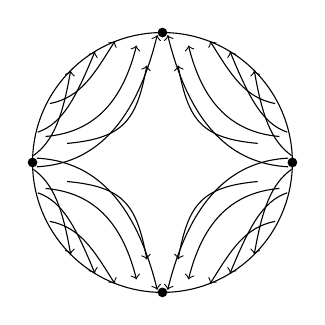
\begin{tikzpicture}[scale=1.1]
  % right figure: electric field lines (from +lambda at left/right to -lambda at top/bottom)
  \draw (0,0) circle (1.5);
  % quadrant I: lines from +lambda at (1.5,0) to -lambda at (0,1.5)
  \draw[->] (1.49,0.08) .. controls (1.25,0.25) and (1.15,0.55) .. (1.06,1.06);
  \draw[->] (1.44,0.35) .. controls (1.15,0.45) and (1.0,0.75) .. (0.78,1.28);
  \draw[->] (1.30,0.68) .. controls (0.95,0.75) and (0.80,1.0) .. (0.55,1.40);
  \draw[->] (1.35,0.30) .. controls (0.75,0.35) and (0.45,0.75) .. (0.30,1.35);
  \draw[->] (1.10,0.22) .. controls (0.45,0.28) and (0.30,0.48) .. (0.18,1.12);
  \draw[->] (1.45,-0.05) .. controls (0.9,-0.02) and (0.35,0.30) .. (0.06,1.47);
  % quadrant II: from +lambda at (-1.5,0) to -lambda at (0,1.5)
  \draw[->] (-1.49,0.08) .. controls (-1.25,0.25) and (-1.15,0.55) .. (-1.06,1.06);
  \draw[->] (-1.44,0.35) .. controls (-1.15,0.45) and (-1.0,0.75) .. (-0.78,1.28);
  \draw[->] (-1.30,0.68) .. controls (-0.95,0.75) and (-0.80,1.0) .. (-0.55,1.40);
  \draw[->] (-1.35,0.30) .. controls (-0.75,0.35) and (-0.45,0.75) .. (-0.30,1.35);
  \draw[->] (-1.10,0.22) .. controls (-0.45,0.28) and (-0.30,0.48) .. (-0.18,1.12);
  \draw[->] (-1.45,-0.05) .. controls (-0.9,-0.02) and (-0.35,0.30) .. (-0.06,1.47);
  % quadrant III: from +lambda at (-1.5,0) to -lambda at (0,-1.5)
  \draw[->] (-1.49,-0.08) .. controls (-1.25,-0.25) and (-1.15,-0.55) .. (-1.06,-1.06);
  \draw[->] (-1.44,-0.35) .. controls (-1.15,-0.45) and (-1.0,-0.75) .. (-0.78,-1.28);
  \draw[->] (-1.30,-0.68) .. controls (-0.95,-0.75) and (-0.80,-1.0) .. (-0.55,-1.40);
  \draw[->] (-1.35,-0.30) .. controls (-0.75,-0.35) and (-0.45,-0.75) .. (-0.30,-1.35);
  \draw[->] (-1.10,-0.22) .. controls (-0.45,-0.28) and (-0.30,-0.48) .. (-0.18,-1.12);
  \draw[->] (-1.45,0.05) .. controls (-0.9,0.02) and (-0.35,-0.30) .. (-0.06,-1.47);
  % quadrant IV: from +lambda at (1.5,0) to -lambda at (0,-1.5)
  \draw[->] (1.49,-0.08) .. controls (1.25,-0.25) and (1.15,-0.55) .. (1.06,-1.06);
  \draw[->] (1.44,-0.35) .. controls (1.15,-0.45) and (1.0,-0.75) .. (0.78,-1.28);
  \draw[->] (1.30,-0.68) .. controls (0.95,-0.75) and (0.80,-1.0) .. (0.55,-1.40);
  \draw[->] (1.35,-0.30) .. controls (0.75,-0.35) and (0.45,-0.75) .. (0.30,-1.35);
  \draw[->] (1.10,-0.22) .. controls (0.45,-0.28) and (0.30,-0.48) .. (0.18,-1.12);
  \draw[->] (1.45,0.05) .. controls (0.9,0.02) and (0.35,-0.30) .. (0.06,-1.47);
  \fill (1.5,0) circle (1.6pt);
  \fill (-1.5,0) circle (1.6pt);
  \fill (0,1.5) circle (1.6pt);
  \fill (0,-1.5) circle (1.6pt);
\end{tikzpicture}
\par\vspace{0.5em}\textbf{Problem 2.20}
\end{center}

The charge density in two dimensions can be expressed as
\[
\sigma(\rho,\phi)=\frac{\lambda}{a}\sum_{n=0}^{3}(-1)^{n}\,\delta(\rho-a)\,\delta(\phi-n\pi/2)
\]
\begin{enumerate}
\item[(a)] Using the Green function expansion from Problem 2.17c, show that the electrostatic potential is
\[
\Phi(\rho,\phi)=\frac{\lambda}{\pi\epsilon_{0}}\sum_{k=0}^{\infty}\frac{1}{2k+1}\left(\frac{\rho_{<}}{\rho_{>}}\right)^{4k+2}\cos[(4k+2)\,\phi]
\]
\item[(b)] Relate the solution of part a to the real part of the complex function
\[
w(z)=\frac{2\lambda}{4\pi\epsilon_{0}}\ln\left[\frac{(z-ia)(z+ia)}{(z-a)(z+a)}\right]
\]
where $z=x+iy=\rho e^{i\phi}$. Comment on the connection to Problem 2.3.
\item[(c)] Find expressions for the Cartesian components of the electric field near the origin, expressed in terms of $x$ and $y$. Keep the $k=0$ and $k=1$ terms in the expansion. For $y=0$ what is the relative magnitude of the $k=1$ ($2^{6}$-pole) contribution to $E_{x}$ compared to the $k=0$ ($2^{2}$-pole or quadrupole) term?
\end{enumerate}
\solution
\textbf{(a)} The source integral has measure $\rho'\,d\rho'\,d\phi'$,
so the factor $\lambda/a$ in the density assigns line charge
$(-1)^n\lambda$ to each point on $\rho'=a$. Their total charge is
zero, eliminating the logarithmic zero mode of $G$. The angular sum is
\[
\sum_{n=0}^3(-1)^n e^{-imn\pi/2}
=\begin{cases}4,&m=4k+2,\\0,&\text{otherwise}.
\end{cases}
\]
Indeed it is the four-term geometric sum with ratio $-e^{-im\pi/2}$,
which is zero unless the ratio is one. With
$t=\min(\rho,a)/\max(\rho,a)$, the remaining Green-function terms give
\[
\Phi=\frac{\lambda}{4\pi\epsilon _0}
       2\sum_{k\geq0}\frac{4t^{4k+2}}{4k+2}\cos[(4k+2)\phi]
=\boxed{\frac{\lambda}{\pi\epsilon _0}\sum_{k\geq0}
       \frac{t^{4k+2}}{2k+1}\cos[(4k+2)\phi].}
\]
\textbf{(b)} Taking the real part of the stated analytic function
uses $\operatorname{Re}\ln(z-z_j)=\ln|z-z_j|$ and gives
\[
\operatorname{Re}w=\frac{\lambda}{2\pi\epsilon _0}
 \ln\frac{|z-ia|\,|z+ia|}{|z-a|\,|z+a|},
\]
which is the sum of the four line-charge potentials. For $|z|<a$,
\[
\ln\frac{z^2+a^2}{z^2-a^2}
=\text{pure imaginary constant}
 +\ln\frac{1+z^2/a^2}{1-z^2/a^2}
=\text{constant}+2\sum_{k\geq0}\frac{(z/a)^{4k+2}}{2k+1}.
\]
For $|z|>a$ expand in $a^2/z^2$ instead; its real part has the same
cosines. These two expansions reproduce part (a).
The four alternating line sources are the same image construction
as in Problem 2.3 when $x_0=y_0$, after rotating the axes by $\pi/4$
and choosing the corresponding length scale. Here the zero-potential
planes are the diagonals between the charged axes.
\textbf{(c)} Keeping $k=0,1$ inside the source circle gives
\[
\Phi=\frac{\lambda}{\pi\epsilon _0}
 \left[\frac{x^2-y^2}{a^2}
 +\frac{x^6-15x^4y^2+15x^2y^4-y^6}{3a^6}
 +O(\rho^{10}/a^{10})\right].
\]
Termwise Cartesian differentiation gives
\[
\boxed{\begin{aligned}
E_x&=-\frac{2\lambda}{\pi\epsilon _0a^2}
 \left[x+\frac{x^5-10x^3y^2+5xy^4}{a^4}\right]
 +O\!\left(\frac{\lambda\rho^9}{\epsilon _0a^{10}}\right),\\
E_y&=\frac{2\lambda}{\pi\epsilon _0a^2}
 \left[y+\frac{5x^4y-10x^2y^3+y^5}{a^4}\right]
 +O\!\left(\frac{\lambda\rho^9}{\epsilon _0a^{10}}\right).
\end{aligned}}
\]
On $y=0$ their two $E_x$ contributions have the same sign and
\[
\boxed{\left|\frac{E_x^{(k=1)}}{E_x^{(k=0)}}\right|=(x/a)^4}
\]
for $x\ne0$, with limiting ratio zero at the origin.

\Needspace{5\baselineskip}
\par\bigskip
\noindent\textbf{2.21}\quad Use Cauchy's theorem to derive the Poisson integral solution. Cauchy's theorem states that if $F(z)$ is analytic in a region $R$ bounded by a closed curve $C$, then
\[
\frac{1}{2\pi i}\oint_{C}\frac{F(z')\;dz'}{z'-z}=\begin{cases}F(z) & \text{if $z$ is inside } R\\ 0 & \text{outside}\end{cases}
\]
\emph{Hint}: You may wish to add an integral that vanishes (associated with the image point) to the integral for the point inside the circle.
\solution
Let $F$ be analytic in the disk $|\zeta|<b$, continuous on its
boundary, and let $\Phi=\operatorname{Re}F$. Fix an interior point
$z$ and its exterior image $z_i=b^2/\bar z$. By Cauchy's formula,
\[
F(z)=\frac1{2\pi i}\oint_{|\zeta|=b}
 F(\zeta)\left[\frac1{\zeta-z}-\frac1{\zeta-z_i}\right]d\zeta.
\]
The second integral is zero because its pole is outside the disk.
Put $\zeta=be^{i\phi'}$, $d\zeta=i\zeta\,d\phi'$. Since
$\zeta\bar\zeta=b^2$ on the contour,
\[
-\frac\zeta{\zeta-b^2/\bar z}
=\frac{\bar z}{\bar\zeta-\bar z}.
\]
Consequently the two kernels combine to a real quantity:
\begin{align*}
\frac\zeta{\zeta-z}+\frac{\bar z}{\bar\zeta-\bar z}
&=\frac{\zeta(\bar\zeta-\bar z)+\bar z(\zeta-z)}{|\zeta-z|^2}\\
&=\frac{b^2-|z|^2}{|\zeta-z|^2}.
\end{align*}
Taking real parts now removes the otherwise unknown harmonic
conjugate of the boundary potential. With $z=\rho e^{i\phi}$,
\[
\boxed{\Phi(\rho,\phi)=\frac1{2\pi}\int_0^{2\pi}
 \Phi(b,\phi')\frac{b^2-\rho^2}
 {b^2+\rho^2-2b\rho\cos(\phi-\phi')}\,d\phi'.}
\]
At $z=0$ the image is understood as a limit at infinity and the
kernel is one, giving the average boundary value. Every harmonic
potential in the simply connected disk has a harmonic conjugate,
so this establishes the Poisson formula for the stated Dirichlet
problem; piecewise boundary data follow by taking interior limits.

\Needspace{5\baselineskip}
\par\bigskip
\noindent\textbf{2.22}\quad\begin{enumerate}
\item[(a)] For the example of oppositely charged conducting hemispherical shells separated by a tiny gap, as shown in Figure 2.8, show that the interior potential ($r<a$) on the $z$ axis is
\[
\Phi_{\mathrm{in}}(z)=V\,\frac{a}{z}\left[1-\frac{(a^{2}-z^{2})}{a\sqrt{a^{2}+z^{2}}}\right]
\]
Find the first few terms of the expansion in powers of $z$ and show that they agree with (2.27) with the appropriate substitutions.
\item[(b)] From the result of part a and (2.22), show that the \erratum{axial electric field $E_z$ (equal to $E_r$ on the positive $z$ axis)} is
\[
\erratum{E_{z}}(z)=\frac{Va^{2}}{(z^{2}+a^{2})^{3/2}}\left(3+\frac{a^{2}}{z^{2}}\right)
\]
for $z>a$, and
\[
\erratum{E_{z}}(z)=-\frac{V}{a}\left[\frac{3+(a/z)^{2}}{(1+(z/a)^{2})^{3/2}}-\frac{a^{2}}{z^{2}}\right]
\]
for $|z|<a$. Show that the second form is well behaved at the origin, with the value $\erratum{E_{z}}(0)=-3V/2a$. Show that at $z=a$ (north pole inside) it has the value $-(\sqrt{2}-1)V/a$. Show that the radial field at the north pole outside has the value $\sqrt{2}\,V/a$.
\item[(c)] Make a sketch of the electric field lines, both inside and outside the conducting hemispheres, with directions indicated. Make a \emph{plot} of the \erratum{axial electric field $E_z$} along the $z$ axis from $z=-2a$ to $z=+2a$.
\end{enumerate}
\solution
The northern hemisphere is at $+V$ and the southern at $-V$.
\textbf{(a)} The interior spherical Poisson kernel gives, on the axis,
\[
\Phi_{\rm in}(z)=\frac{Va(a^2-z^2)}2
 \int_{-1}^{1}\frac{\operatorname{sgn}u\,du}
                 {(a^2+z^2-2azu)^{3/2}},\qquad |z|<a.
\]
For $z\ne0$, the integral is
\[
\frac1{az}\left[\frac1{a-z}+\frac1{a+z}
                              -\frac2{\sqrt{a^2+z^2}}\right].
\]
Combining the first two fractions before multiplying the prefactor
therefore gives
\[
\boxed{\Phi_{\rm in}(z)=\frac{Va}{z}
 \left[1-\frac{a^2-z^2}{a\sqrt{a^2+z^2}}\right].}
\]
Put $t=z/a$ and expand
$(1+t^2)^{-1/2}=1-t^2/2+3t^4/8-5t^6/16+35t^8/128+\cdots$.
Multiplication by $1-t^2$ and division by $t$ give
\[
\frac{\Phi_{\rm in}}V=\frac32t-\frac78t^3+\frac{11}{16}t^5
                              -\frac{75}{128}t^7+O(t^9).
\]
The interior and exterior harmonic expansions are related by Kelvin
inversion,
$\Phi_{\rm out}(r,\theta)=(a/r)\Phi_{\rm in}(a^2/r,\theta)$.
Thus the exterior terms are
$V[\tfrac32(a/r)^2P_1(\cos\theta)
-\tfrac78(a/r)^4P_3(\cos\theta)+\cdots]$.
On the positive axis $P_l(1)=1$, so the replacements
$(a/r)^{l+1}\mapsto(r/a)^l$ recover the interior coefficients above
from (2.27).

\textbf{(b)} Differentiating the interior expression at fixed sign
of $z$ gives the axial component
\[
\boxed{E_z^{\rm in}(z)=-\frac Va
 \left[\frac{3+(a/z)^2}{[1+(z/a)^2]^{3/2}}-\frac{a^2}{z^2}\right].}
\]
Its apparently singular terms cancel. In fact differentiating the
power series gives
\[
E_z^{\rm in}(z)=\frac Va\left[-\frac32+\frac{21}{8}t^2
                     -\frac{55}{16}t^4+\frac{525}{128}t^6+O(t^8)\right].
\]
The origin value is therefore $-3V/(2a)$.
The exterior positive-axis potential (2.22), also obtained by the
inversion above, is
\[
\Phi_{\rm out}(z)=V\left[1-
             \frac{z^2-a^2}{z\sqrt{z^2+a^2}}\right],\quad z>a.
\]
Its derivative is
\[
\boxed{E_z^{\rm out}(z)=\frac{Va^2}{(z^2+a^2)^{3/2}}
                         \left(3+\frac{a^2}{z^2}\right),\quad z>a.}
\]
On the positive axis $E_z=E_r$. At the north pole the limiting
values are $E_r(a^-)=-\left(\sqrt2-1\right)V/a$ and
$E_r(a^+)=\sqrt2 V/a$, agreeing with the question. Their difference
is $(2\sqrt2-1)V/a$, the surface charge divided by $\epsilon _0$.

\textbf{(c)} Antisymmetry of the potential,
$\Phi(-z)=-\Phi(z)$, implies $E_z(-z)=E_z(z)$. The radial basis
vector reverses on the negative axis, so strictly
$E_r(z)=\operatorname{sgn}(z)E_z(z)$ for $z\ne0$; $E_r$ has no
single basis direction at the origin. The finite origin value is the continuous \emph{axial} component;
the statement uses corrected notation to make this distinction explicit. The plot shows that
component together with the true radial component on the negative
axis, where they differ. Fields jump at $z=\pm a$; there is no field
value inside an ideal zero-thickness metal surface itself.
\begin{center}
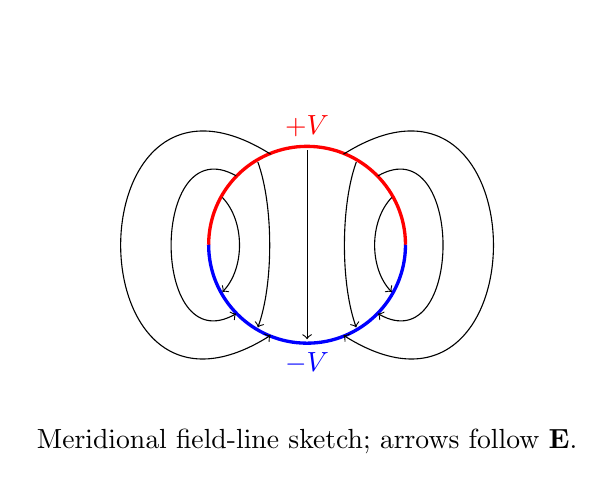
\begin{tikzpicture}[scale=1.25]
\draw[very thick,red] (0:1) arc (0:180:1);
\draw[very thick,blue] (180:1) arc (180:360:1);
\node[red,above] at (0,1) {$+V$};\node[blue,below] at (0,-1) {$-V$};
\draw[->] (0,.96)--(0,-.96);
\foreach \s in {-1,1} {
 \draw[->] ({\s*.5},.84) .. controls ({\s*.34},.4) and ({\s*.34},-.4) .. ({\s*.5},-.84);
 \draw[->] ({\s*.86},.48) .. controls ({\s*.63},.24) and ({\s*.63},-.24) .. ({\s*.86},-.48);
 \draw[->] ({\s*.72},.70) .. controls ({\s*1.6},1.20) and ({\s*1.6},-1.20) .. ({\s*.72},-.70);
 \draw[->] ({\s*.37},.92) .. controls ({\s*2.4},2.2) and ({\s*2.4},-2.2) .. ({\s*.37},-.92);
}
\node at (0,-2.0) {Meridional field-line sketch; arrows follow $\mathbf E$.};
\end{tikzpicture}
\par\medskip
% Generated by supplementary/check_ch02.py --write-assets
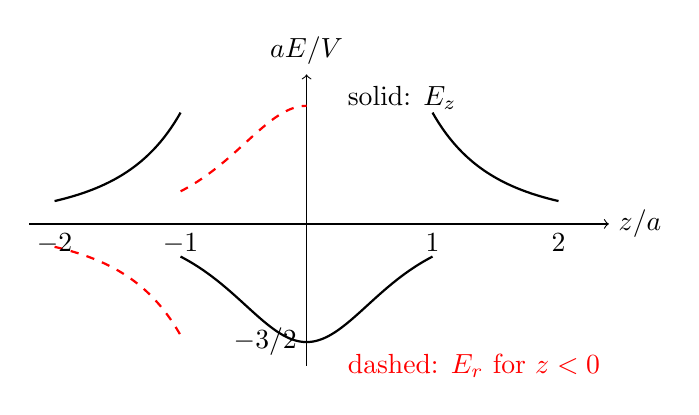
\begin{tikzpicture}[x=1.6cm,y=1cm]
\draw[->] (-2.2,0)--(2.4,0) node[right] {$z/a$};
\draw[->] (0,-1.8)--(0,1.9) node[above] {$aE/V$};
\draw[black,thick] plot coordinates {(-2.000000,0.290689) (-1.989899,0.294470) (-1.979798,0.298314) (-1.969697,0.302223) (-1.959596,0.306198) (-1.949495,0.310241) (-1.939394,0.314353) (-1.929293,0.318535) (-1.919192,0.322789) (-1.909091,0.327116) (-1.898990,0.331518) (-1.888889,0.335997) (-1.878788,0.340554) (-1.868687,0.345190) (-1.858586,0.349908) (-1.848485,0.354708) (-1.838384,0.359594) (-1.828283,0.364567) (-1.818182,0.369628) (-1.808081,0.374779) (-1.797980,0.380023) (-1.787879,0.385361) (-1.777778,0.390796) (-1.767677,0.396330) (-1.757576,0.401964) (-1.747475,0.407702) (-1.737374,0.413545) (-1.727273,0.419495) (-1.717172,0.425556) (-1.707071,0.431729) (-1.696970,0.438017) (-1.686869,0.444423) (-1.676768,0.450949) (-1.666667,0.457599) (-1.656566,0.464374) (-1.646465,0.471278) (-1.636364,0.478314) (-1.626263,0.485485) (-1.616162,0.492794) (-1.606061,0.500244) (-1.595960,0.507838) (-1.585859,0.515581) (-1.575758,0.523475) (-1.565657,0.531524) (-1.555556,0.539732) (-1.545455,0.548102) (-1.535354,0.556639) (-1.525253,0.565346) (-1.515152,0.574228) (-1.505051,0.583289) (-1.494949,0.592533) (-1.484848,0.601964) (-1.474747,0.611589) (-1.464646,0.621410) (-1.454545,0.631434) (-1.444444,0.641665) (-1.434343,0.652108) (-1.424242,0.662769) (-1.414141,0.673654) (-1.404040,0.684768) (-1.393939,0.696116) (-1.383838,0.707706) (-1.373737,0.719544) (-1.363636,0.731635) (-1.353535,0.743987) (-1.343434,0.756606) (-1.333333,0.769500) (-1.323232,0.782676) (-1.313131,0.796141) (-1.303030,0.809904) (-1.292929,0.823972) (-1.282828,0.838355) (-1.272727,0.853060) (-1.262626,0.868096) (-1.252525,0.883473) (-1.242424,0.899201) (-1.232323,0.915289) (-1.222222,0.931747) (-1.212121,0.948587) (-1.202020,0.965819) (-1.191919,0.983455) (-1.181818,1.001507) (-1.171717,1.019987) (-1.161616,1.038907) (-1.151515,1.058282) (-1.141414,1.078124) (-1.131313,1.098448) (-1.121212,1.119270) (-1.111111,1.140603) (-1.101010,1.162466) (-1.090909,1.184873) (-1.080808,1.207843) (-1.070707,1.231395) (-1.060606,1.255545) (-1.050505,1.280316) (-1.040404,1.305726) (-1.030303,1.331798) (-1.020202,1.358554) (-1.010101,1.386018) (-1.000000,1.414214)};
\draw[red,dashed,thick] plot coordinates {(-2.000000,-0.290689) (-1.989899,-0.294470) (-1.979798,-0.298314) (-1.969697,-0.302223) (-1.959596,-0.306198) (-1.949495,-0.310241) (-1.939394,-0.314353) (-1.929293,-0.318535) (-1.919192,-0.322789) (-1.909091,-0.327116) (-1.898990,-0.331518) (-1.888889,-0.335997) (-1.878788,-0.340554) (-1.868687,-0.345190) (-1.858586,-0.349908) (-1.848485,-0.354708) (-1.838384,-0.359594) (-1.828283,-0.364567) (-1.818182,-0.369628) (-1.808081,-0.374779) (-1.797980,-0.380023) (-1.787879,-0.385361) (-1.777778,-0.390796) (-1.767677,-0.396330) (-1.757576,-0.401964) (-1.747475,-0.407702) (-1.737374,-0.413545) (-1.727273,-0.419495) (-1.717172,-0.425556) (-1.707071,-0.431729) (-1.696970,-0.438017) (-1.686869,-0.444423) (-1.676768,-0.450949) (-1.666667,-0.457599) (-1.656566,-0.464374) (-1.646465,-0.471278) (-1.636364,-0.478314) (-1.626263,-0.485485) (-1.616162,-0.492794) (-1.606061,-0.500244) (-1.595960,-0.507838) (-1.585859,-0.515581) (-1.575758,-0.523475) (-1.565657,-0.531524) (-1.555556,-0.539732) (-1.545455,-0.548102) (-1.535354,-0.556639) (-1.525253,-0.565346) (-1.515152,-0.574228) (-1.505051,-0.583289) (-1.494949,-0.592533) (-1.484848,-0.601964) (-1.474747,-0.611589) (-1.464646,-0.621410) (-1.454545,-0.631434) (-1.444444,-0.641665) (-1.434343,-0.652108) (-1.424242,-0.662769) (-1.414141,-0.673654) (-1.404040,-0.684768) (-1.393939,-0.696116) (-1.383838,-0.707706) (-1.373737,-0.719544) (-1.363636,-0.731635) (-1.353535,-0.743987) (-1.343434,-0.756606) (-1.333333,-0.769500) (-1.323232,-0.782676) (-1.313131,-0.796141) (-1.303030,-0.809904) (-1.292929,-0.823972) (-1.282828,-0.838355) (-1.272727,-0.853060) (-1.262626,-0.868096) (-1.252525,-0.883473) (-1.242424,-0.899201) (-1.232323,-0.915289) (-1.222222,-0.931747) (-1.212121,-0.948587) (-1.202020,-0.965819) (-1.191919,-0.983455) (-1.181818,-1.001507) (-1.171717,-1.019987) (-1.161616,-1.038907) (-1.151515,-1.058282) (-1.141414,-1.078124) (-1.131313,-1.098448) (-1.121212,-1.119270) (-1.111111,-1.140603) (-1.101010,-1.162466) (-1.090909,-1.184873) (-1.080808,-1.207843) (-1.070707,-1.231395) (-1.060606,-1.255545) (-1.050505,-1.280316) (-1.040404,-1.305726) (-1.030303,-1.331798) (-1.020202,-1.358554) (-1.010101,-1.386018) (-1.000000,-1.414214)};
\draw[black,thick] plot coordinates {(-0.999999,-0.414214) (-0.989898,-0.422655) (-0.979797,-0.431243) (-0.969696,-0.439979) (-0.959595,-0.448865) (-0.949494,-0.457901) (-0.939393,-0.467090) (-0.929292,-0.476432) (-0.919191,-0.485928) (-0.909090,-0.495579) (-0.898989,-0.505387) (-0.888888,-0.515352) (-0.878787,-0.525475) (-0.868686,-0.535756) (-0.858585,-0.546196) (-0.848484,-0.556795) (-0.838383,-0.567554) (-0.828282,-0.578471) (-0.818181,-0.589548) (-0.808080,-0.600784) (-0.797979,-0.612179) (-0.787878,-0.623732) (-0.777777,-0.635442) (-0.767676,-0.647308) (-0.757575,-0.659329) (-0.747474,-0.671503) (-0.737373,-0.683830) (-0.727272,-0.696307) (-0.717171,-0.708932) (-0.707070,-0.721702) (-0.696969,-0.734616) (-0.686868,-0.747669) (-0.676767,-0.760860) (-0.666666,-0.774184) (-0.656565,-0.787637) (-0.646464,-0.801217) (-0.636363,-0.814917) (-0.626262,-0.828735) (-0.616161,-0.842663) (-0.606060,-0.856698) (-0.595959,-0.870832) (-0.585858,-0.885061) (-0.575757,-0.899378) (-0.565656,-0.913776) (-0.555555,-0.928247) (-0.545454,-0.942784) (-0.535353,-0.957379) (-0.525252,-0.972023) (-0.515151,-0.986709) (-0.505050,-1.001426) (-0.494949,-1.016165) (-0.484848,-1.030916) (-0.474747,-1.045669) (-0.464646,-1.060414) (-0.454545,-1.075138) (-0.444444,-1.089831) (-0.434343,-1.104481) (-0.424242,-1.119076) (-0.414141,-1.133603) (-0.404040,-1.148049) (-0.393939,-1.162401) (-0.383838,-1.176647) (-0.373737,-1.190771) (-0.363636,-1.204761) (-0.353535,-1.218602) (-0.343434,-1.232280) (-0.333333,-1.245780) (-0.323232,-1.259087) (-0.313131,-1.272188) (-0.303030,-1.285065) (-0.292929,-1.297706) (-0.282828,-1.310094) (-0.272727,-1.322214) (-0.262626,-1.334053) (-0.252525,-1.345594) (-0.242424,-1.356823) (-0.232323,-1.367725) (-0.222222,-1.378286) (-0.212121,-1.388491) (-0.202020,-1.398327) (-0.191919,-1.407780) (-0.181818,-1.416837) (-0.171717,-1.425484) (-0.161616,-1.433710) (-0.151515,-1.441502) (-0.141414,-1.448848) (-0.131313,-1.455738) (-0.121212,-1.462162) (-0.111111,-1.468109) (-0.101010,-1.473571) (-0.090909,-1.478538) (-0.080808,-1.483004) (-0.070707,-1.486962) (-0.060606,-1.490404) (-0.050505,-1.493327) (-0.040404,-1.495724) (-0.030303,-1.497592) (-0.020202,-1.498929) (-0.010101,-1.499732) (0.000000,-1.500000)};
\draw[red,dashed,thick] plot coordinates {(-0.999999,0.414214) (-0.989898,0.422655) (-0.979797,0.431243) (-0.969696,0.439979) (-0.959595,0.448865) (-0.949494,0.457901) (-0.939393,0.467090) (-0.929292,0.476432) (-0.919191,0.485928) (-0.909090,0.495579) (-0.898989,0.505387) (-0.888888,0.515352) (-0.878787,0.525475) (-0.868686,0.535756) (-0.858585,0.546196) (-0.848484,0.556795) (-0.838383,0.567554) (-0.828282,0.578471) (-0.818181,0.589548) (-0.808080,0.600784) (-0.797979,0.612179) (-0.787878,0.623732) (-0.777777,0.635442) (-0.767676,0.647308) (-0.757575,0.659329) (-0.747474,0.671503) (-0.737373,0.683830) (-0.727272,0.696307) (-0.717171,0.708932) (-0.707070,0.721702) (-0.696969,0.734616) (-0.686868,0.747669) (-0.676767,0.760860) (-0.666666,0.774184) (-0.656565,0.787637) (-0.646464,0.801217) (-0.636363,0.814917) (-0.626262,0.828735) (-0.616161,0.842663) (-0.606060,0.856698) (-0.595959,0.870832) (-0.585858,0.885061) (-0.575757,0.899378) (-0.565656,0.913776) (-0.555555,0.928247) (-0.545454,0.942784) (-0.535353,0.957379) (-0.525252,0.972023) (-0.515151,0.986709) (-0.505050,1.001426) (-0.494949,1.016165) (-0.484848,1.030916) (-0.474747,1.045669) (-0.464646,1.060414) (-0.454545,1.075138) (-0.444444,1.089831) (-0.434343,1.104481) (-0.424242,1.119076) (-0.414141,1.133603) (-0.404040,1.148049) (-0.393939,1.162401) (-0.383838,1.176647) (-0.373737,1.190771) (-0.363636,1.204761) (-0.353535,1.218602) (-0.343434,1.232280) (-0.333333,1.245780) (-0.323232,1.259087) (-0.313131,1.272188) (-0.303030,1.285065) (-0.292929,1.297706) (-0.282828,1.310094) (-0.272727,1.322214) (-0.262626,1.334053) (-0.252525,1.345594) (-0.242424,1.356823) (-0.232323,1.367725) (-0.222222,1.378286) (-0.212121,1.388491) (-0.202020,1.398327) (-0.191919,1.407780) (-0.181818,1.416837) (-0.171717,1.425484) (-0.161616,1.433710) (-0.151515,1.441502) (-0.141414,1.448848) (-0.131313,1.455738) (-0.121212,1.462162) (-0.111111,1.468109) (-0.101010,1.473571) (-0.090909,1.478538) (-0.080808,1.483004) (-0.070707,1.486962) (-0.060606,1.490404) (-0.050505,1.493327) (-0.040404,1.495724) (-0.030303,1.497592) (-0.020202,1.498929) (-0.010101,1.499732) (0.000000,1.500000)};
\draw[black,thick] plot coordinates {(0.000000,-1.500000) (0.010101,-1.499732) (0.020202,-1.498929) (0.030303,-1.497592) (0.040404,-1.495724) (0.050505,-1.493327) (0.060606,-1.490404) (0.070707,-1.486962) (0.080808,-1.483004) (0.090909,-1.478538) (0.101010,-1.473571) (0.111111,-1.468109) (0.121212,-1.462162) (0.131313,-1.455738) (0.141414,-1.448848) (0.151515,-1.441502) (0.161616,-1.433710) (0.171717,-1.425484) (0.181818,-1.416837) (0.191919,-1.407780) (0.202020,-1.398327) (0.212121,-1.388491) (0.222222,-1.378286) (0.232323,-1.367725) (0.242424,-1.356823) (0.252525,-1.345594) (0.262626,-1.334053) (0.272727,-1.322214) (0.282828,-1.310094) (0.292929,-1.297706) (0.303030,-1.285065) (0.313131,-1.272188) (0.323232,-1.259087) (0.333333,-1.245780) (0.343434,-1.232280) (0.353535,-1.218602) (0.363636,-1.204761) (0.373737,-1.190771) (0.383838,-1.176647) (0.393939,-1.162401) (0.404040,-1.148049) (0.414141,-1.133603) (0.424242,-1.119076) (0.434343,-1.104481) (0.444444,-1.089831) (0.454545,-1.075138) (0.464646,-1.060414) (0.474747,-1.045669) (0.484848,-1.030916) (0.494949,-1.016165) (0.505050,-1.001426) (0.515151,-0.986709) (0.525252,-0.972023) (0.535353,-0.957379) (0.545454,-0.942784) (0.555555,-0.928247) (0.565656,-0.913776) (0.575757,-0.899378) (0.585858,-0.885061) (0.595959,-0.870832) (0.606060,-0.856698) (0.616161,-0.842663) (0.626262,-0.828735) (0.636363,-0.814917) (0.646464,-0.801217) (0.656565,-0.787637) (0.666666,-0.774184) (0.676767,-0.760860) (0.686868,-0.747669) (0.696969,-0.734616) (0.707070,-0.721702) (0.717171,-0.708932) (0.727272,-0.696307) (0.737373,-0.683830) (0.747474,-0.671503) (0.757575,-0.659329) (0.767676,-0.647308) (0.777777,-0.635442) (0.787878,-0.623732) (0.797979,-0.612179) (0.808080,-0.600784) (0.818181,-0.589548) (0.828282,-0.578471) (0.838383,-0.567554) (0.848484,-0.556795) (0.858585,-0.546196) (0.868686,-0.535756) (0.878787,-0.525475) (0.888888,-0.515352) (0.898989,-0.505387) (0.909090,-0.495579) (0.919191,-0.485928) (0.929292,-0.476432) (0.939393,-0.467090) (0.949494,-0.457901) (0.959595,-0.448865) (0.969696,-0.439979) (0.979797,-0.431243) (0.989898,-0.422655) (0.999999,-0.414214)};
\draw[black,thick] plot coordinates {(1.000000,1.414214) (1.010101,1.386018) (1.020202,1.358554) (1.030303,1.331798) (1.040404,1.305726) (1.050505,1.280316) (1.060606,1.255545) (1.070707,1.231395) (1.080808,1.207843) (1.090909,1.184873) (1.101010,1.162466) (1.111111,1.140603) (1.121212,1.119270) (1.131313,1.098448) (1.141414,1.078124) (1.151515,1.058282) (1.161616,1.038907) (1.171717,1.019987) (1.181818,1.001507) (1.191919,0.983455) (1.202020,0.965819) (1.212121,0.948587) (1.222222,0.931747) (1.232323,0.915289) (1.242424,0.899201) (1.252525,0.883473) (1.262626,0.868096) (1.272727,0.853060) (1.282828,0.838355) (1.292929,0.823972) (1.303030,0.809904) (1.313131,0.796141) (1.323232,0.782676) (1.333333,0.769500) (1.343434,0.756606) (1.353535,0.743987) (1.363636,0.731635) (1.373737,0.719544) (1.383838,0.707706) (1.393939,0.696116) (1.404040,0.684768) (1.414141,0.673654) (1.424242,0.662769) (1.434343,0.652108) (1.444444,0.641665) (1.454545,0.631434) (1.464646,0.621410) (1.474747,0.611589) (1.484848,0.601964) (1.494949,0.592533) (1.505051,0.583289) (1.515152,0.574228) (1.525253,0.565346) (1.535354,0.556639) (1.545455,0.548102) (1.555556,0.539732) (1.565657,0.531524) (1.575758,0.523475) (1.585859,0.515581) (1.595960,0.507838) (1.606061,0.500244) (1.616162,0.492794) (1.626263,0.485485) (1.636364,0.478314) (1.646465,0.471278) (1.656566,0.464374) (1.666667,0.457599) (1.676768,0.450949) (1.686869,0.444423) (1.696970,0.438017) (1.707071,0.431729) (1.717172,0.425556) (1.727273,0.419495) (1.737374,0.413545) (1.747475,0.407702) (1.757576,0.401964) (1.767677,0.396330) (1.777778,0.390796) (1.787879,0.385361) (1.797980,0.380023) (1.808081,0.374779) (1.818182,0.369628) (1.828283,0.364567) (1.838384,0.359594) (1.848485,0.354708) (1.858586,0.349908) (1.868687,0.345190) (1.878788,0.340554) (1.888889,0.335997) (1.898990,0.331518) (1.909091,0.327116) (1.919192,0.322789) (1.929293,0.318535) (1.939394,0.314353) (1.949495,0.310241) (1.959596,0.306198) (1.969697,0.302223) (1.979798,0.298314) (1.989899,0.294470) (2.000000,0.290689)};
\node[below] at (-2,0) {$ -2 $};
\node[below] at (-1,0) {$ -1 $};
\node[below] at (1,0) {$ 1 $};
\node[below] at (2,0) {$ 2 $};
\node[left] at (0,-1.5) {$-3/2$};
\node[right] at (.25,1.6) {solid: $E_z$};
\node[red,right] at (.25,-1.8) {dashed: $E_r$ for $z<0$};
\end{tikzpicture}

\end{center}
The inside lines run from the northern to the southern inner face;
the outside lines connect the outer faces around the shell. The
sketch illustrates topology; the accompanying axial curves use the
exact formulas above.

\Needspace{5\baselineskip}
\par\bigskip
\noindent\textbf{2.23}\quad A hollow cube has conducting walls defined by six planes $x=0$, $y=0$, $z=0$, and $x=a$, $y=a$, $z=a$. The walls $z=0$ and $z=a$ are held at a constant potential $V$. The other four sides are at zero potential.
\begin{enumerate}
\item[(a)] Find the potential $\Phi(x,y,z)$ at any point inside the cube.
\item[(b)] Evaluate the potential at the center of the cube numerically, accurate to three significant figures. How many terms in the series is it necessary to keep in order to attain this accuracy? Compare your numerical result with the average value of the potential on the walls. See Problem 2.28.
\item[(c)] Find the surface-charge density on the surface $z=a$.
\end{enumerate}
\solution
\textbf{(a)} The four grounded side walls select
$\sin(m\pi x/a)\sin(n\pi y/a)$. For a fixed pair the remaining
separation equation is $Z''-k_{mn}^2Z=0$, where
$k_{mn}=\pi\sqrt{m^2+n^2}/a$. Equal values at $z=0,a$ select
$Z=\cosh[k_{mn}(z-a/2)]/\cosh(k_{mn}a/2)$.
The double sine coefficients of a constant on a square are
\[
\frac4{a^2}\int_0^a\!dx\int_0^a\!dy\,
 V\sin\frac{m\pi x}a\sin\frac{n\pi y}a
=\frac{4V[1-(-1)^m][1-(-1)^n]}{mn\pi^2}.
\]
Thus only odd $m,n$ occur, and
\[
\boxed{\Phi=\frac{16V}{\pi^2}
 \sum_{\substack{m,n\geq1\\m,n\ {\rm odd}}}
 \frac{\sin(m\pi x/a)\sin(n\pi y/a)}{mn}
 \frac{\cosh[k_{mn}(z-a/2)]}{\cosh(k_{mn}a/2)}.}
\]
At the edges the imposed boundary data have different one-sided
limits; the interior solution and the values on open faces are
well defined.
\textbf{(b)} At the center, the two sines supply
$(-1)^{(m+n-2)/2}$. Summing all pairs with $m,n=1,3,\ldots,2N-1$
gives
\[
\begin{array}{c|c|c}
N&\text{number of pairs}&\Phi(a/2,a/2,a/2)/V\\\hline
1&1&0.347545849\\
2&4&0.332957715\\
3&9&0.333345107\\
4&16&0.333332938
\end{array}
\]
The four-pair truncation already rounds to $0.333$ to three
significant figures; it contains only three distinct values after
using $m\leftrightarrow n$ symmetry. There is also an exact check:
by cube symmetry the harmonic response at the center to each
unit-potential face is the same, and the sum of the six responses
is one. Two faces at $V$ therefore give
\[
\boxed{\Phi_{\rm center}=V/3,}
\]
exactly the average wall potential $(V+V)/6$. This proves the
accuracy of the reported truncation without inferring convergence
from successive partial sums alone.
\textbf{(c)} On the inner face $z=a$ the conductor-to-cavity normal
is $-\widehat{\mathbf z}$, giving
$\sigma=\epsilon _0\partial_z\Phi|_{a^-}$. Differentiation yields
\[
\boxed{\sigma(x,y)=\frac{16\epsilon _0V}{\pi^2}
 \sum_{\substack{m,n\geq1\\m,n\ {\rm odd}}}
 \frac{k_{mn}\tanh(k_{mn}a/2)}{mn}
       \sin\frac{m\pi x}a\sin\frac{n\pi y}a.}
\]
The derivative series is understood as its interior limit
$z\uparrow a$, or an equivalent Abel limit, away from edges; charge
crowding makes the ideal sharp-edge density singular. This determines
the cavity-facing charge only, since no exterior boundary problem
was specified.

\Needspace{5\baselineskip}
\par\bigskip
\noindent\textbf{2.24}\quad In the two-dimensional region shown in Fig.~2.12, the angular functions appropriate for Dirichlet boundary conditions at $\phi=0$ and $\phi=\beta$ are $\Phi(\phi)=A_{m}\sin(m\pi\phi/\beta)$. Show that the completeness relation for these functions is
\[
\delta(\phi-\phi')=\frac{2}{\beta}\sum_{m=1}^{\infty}\sin(m\pi\phi/\beta)\,\sin(m\pi\phi'/\beta)\qquad\text{for }0<\phi,\,\phi'<\beta
\]
\solution
For positive integers $m,n$, product-to-sum integration gives
\[
\int_0^\beta\sin\frac{m\pi\phi}\beta\sin\frac{n\pi\phi}\beta\,d\phi
=\frac\beta2\delta_{mn}.
\]
To show that the normalized modes are complete, take a smooth test
function $f$ with support in $(0,\beta)$, extend it oddly to
$(-\beta,\beta)$, and periodically with period $2\beta$.
The ordinary Fourier expansion of this odd function contains only
sines, with coefficients
\[
f_m=\frac2\beta\int_0^\beta f(\phi')
                    \sin\frac{m\pi\phi'}\beta\,d\phi'.
\]
Substituting these coefficients back into the Fourier series yields
\[
f(\phi)=\int_0^\beta\left[\frac2\beta\sum_{m=1}^\infty
 \sin\frac{m\pi\phi}\beta\sin\frac{m\pi\phi'}\beta\right]
 f(\phi')\,d\phi'.
\]
The bracket therefore has precisely the action of the delta
function on every such test function:
\[
\boxed{\delta(\phi-\phi')=\frac2\beta\sum_{m=1}^\infty
 \sin\frac{m\pi\phi}\beta\sin\frac{m\pi\phi'}\beta.}
\]
This is a distributional completeness relation for interior points,
not a pointwise convergent numerical series for the delta function.
The restriction away from the endpoints avoids the half-weight
endpoint convention of Fourier boundary limits.

\Needspace{5\baselineskip}
\par\bigskip
\noindent\textbf{2.25}\quad Two conducting planes at zero potential meet along the $z$ axis, making an angle $\beta$ between them, as in Fig.~2.12. A unit line charge parallel to the $z$ axis is located between the planes at position $(\rho',\phi')$.
\begin{enumerate}
\item[(a)] Show that $(4\pi\epsilon_{0})$ times the potential in the space between the planes, that is, the Dirichlet Green function $G(\rho,\phi;\rho',\phi')$, is given by the infinite series
\[
G(\rho,\phi;\rho',\phi')=4\sum_{m=1}^{\infty}\frac{1}{m}\,\rho_{<}^{m\pi/\beta}\rho_{>}^{-m\pi/\beta}\sin(m\pi\phi/\beta)\,\sin(m\pi\phi'/\beta)
\]
\item[(b)] By means of complex-variable techniques or other means, show that the series can be summed to give a closed form,
\[
G(\rho,\phi;\rho',\phi')=\ln\left\{\frac{(\rho)^{2\pi/\beta}+(\rho')^{2\pi/\beta}-2(\rho\rho')^{\pi/\beta}\cos[\pi(\phi+\phi')/\beta]}{(\rho)^{2\pi/\beta}+(\rho')^{2\pi/\beta}-2(\rho\rho')^{\pi/\beta}\cos[\pi(\phi-\phi')/\beta]}\right\}
\]
\item[(c)] Verify that you obtain the familiar results when $\beta=\pi$ and $\beta=\pi/2$.
\end{enumerate}
\solution
\textbf{(a)} With $\nu_m=m\pi/\beta$, expand
\[
G=\frac2\beta\sum_{m\geq1}g_m(\rho,\rho')
                      \sin(\nu_m\phi)\sin(\nu_m\phi').
\]
Using Problem 2.24, the radial equation is
\[
\frac1{\rho'}(\rho'g_m')'-\frac{\nu_m^2}{\rho'^2}g_m
 =-4\pi\frac{\delta(\rho'-\rho)}\rho.
\]
Boundedness at zero and decay at infinity select
$g_m=A_m\rho_<^{\nu_m}\rho_>^{-\nu_m}$.
The radial derivative jump is $-2\nu_mA_m=-4\pi$, so
$A_m=2\pi/\nu_m$. Multiplying by the angular normalization
$2/\beta$ gives
\[
\boxed{G=4\sum_{m=1}^\infty\frac1m
 \left(\frac{\rho_<}{\rho_>}\right)^{m\pi/\beta}
 \sin\frac{m\pi\phi}\beta\sin\frac{m\pi\phi'}\beta.}
\]
For unit line charge, $\Phi=G/(4\pi\epsilon _0)$.
\textbf{(b)} Put
$t=(\rho_</\rho_>)^{\pi/\beta}$,
$A=\pi\phi/\beta$, and $B=\pi\phi'/\beta$.
Since $2\sin mA\sin mB=\cos m(A-B)-\cos m(A+B)$ and
$\sum_{m\geq1}t^m\cos m\theta/m
=-\tfrac12\ln(1-2t\cos\theta+t^2)$,
\[
G=\ln\frac{1-2t\cos(A+B)+t^2}{1-2t\cos(A-B)+t^2}.
\]
Multiplication of numerator and denominator by
$\rho_>^{2\pi/\beta}$ yields exactly
\[
\boxed{G=\ln\frac{\rho^{2\pi/\beta}+\rho'^{2\pi/\beta}
 -2(\rho\rho')^{\pi/\beta}\cos[\pi(\phi+\phi')/\beta]}
 {\rho^{2\pi/\beta}+\rho'^{2\pi/\beta}
 -2(\rho\rho')^{\pi/\beta}\cos[\pi(\phi-\phi')/\beta]}.}
\]
Equivalently the analytic mapping $w=z^{\pi/\beta}$ sends the wedge
to the upper half-plane; the numerator is the squared distance to
the reflected source in that plane. Near the physical source the
analytic mapping is locally linear, so its scale cancels in the
ratio and the singular term remains $-\ln|z-z'|^2$.
\textbf{(c)} For $\beta=\pi$ the result is
$G=\ln[|z-\bar z'|^2/|z-z'|^2]$, the real line and its negative
mirror in a single plane. For $\beta=\pi/2$, factor the squares:
\[
G=\ln\frac{|z^2-\bar z'^2|^2}{|z^2-z'^2|^2}
 =\ln\frac{|z-\bar z'|^2|z+\bar z'|^2}
              {|z-z'|^2|z+z'|^2}.
\]
These are a positive source at $z'$, a positive image at $-z'$,
and negative images at $\bar z'$ and $-\bar z'$, exactly the
four-line construction of Problem 2.3.

\Needspace{5\baselineskip}
\par\bigskip
\noindent\textbf{2.26}\quad The two-dimensional region, $\rho\geq a$, $0\leq\phi\leq\beta$, is bounded by conducting surfaces at $\phi=0$, $\rho=a$, and $\phi=\beta$ held at zero potential, as indicated in the sketch. At large $\rho$ the potential is determined by some configuration of charges and/or conductors at fixed potentials.

\begin{center}
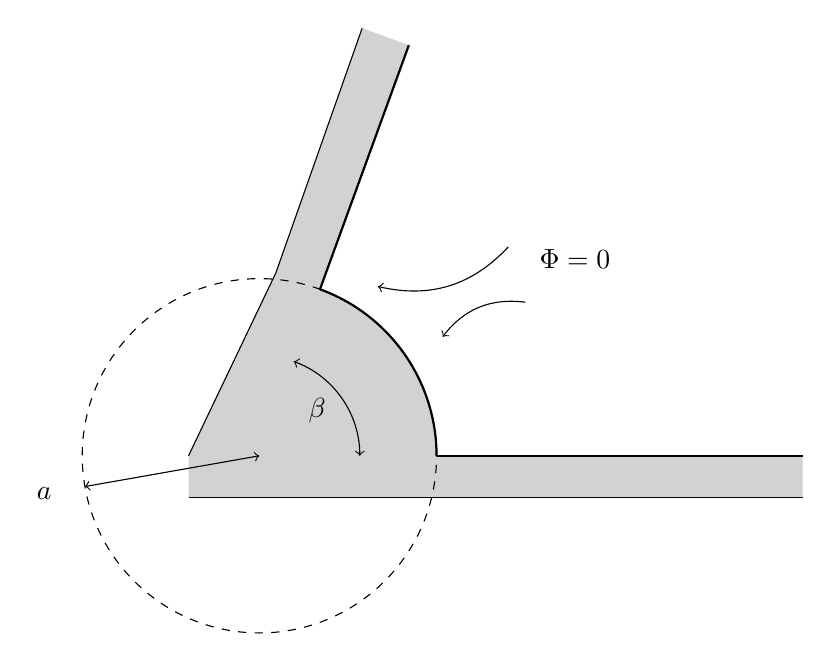
\begin{tikzpicture}[scale=1.5]
  % conductor (shaded): slab below phi=0 plane + sector rho<a + slab beyond phi=beta plane
  \fill[gray!35] (-0.6,0) -- (-0.6,-0.35) -- (4.6,-0.35) -- (4.6,0) -- (1.5,0)
    arc (0:70:1.5) -- (70:3.7) -- ++(160:0.42) -- (0.14,1.55) -- cycle;
  % dashed continuation of the circle rho = a
  \draw[dashed] (0,0) circle (1.5);
  % boundaries of the free region (conducting surfaces)
  \draw[thick] (1.5,0) -- (4.6,0);                    % phi = 0 plane
  \draw[thick] (70:1.5) -- (70:3.7);                  % phi = beta plane
  \draw[thick] (1.5,0) arc (0:70:1.5);                % cylinder surface rho = a
  % outer edges of the conductor block
  \draw[thin] (-0.6,-0.35) -- (4.6,-0.35);
  \draw[thin] (-0.6,0) -- (0.14,1.55);
  \draw[thin] (0.14,1.55) -- (0.87,3.62);
  % radius arrow a
  \draw[<->] (0,0) -- (190:1.5);
  \node at (190:1.85) {$a$};
  % angle beta at the origin
  \draw[<->] (0.85,0) arc (0:70:0.85);
  \node at (38:0.62) {$\beta$};
  % Phi = 0 label with pointers into the free channel
  \node at (32:3.15) {$\Phi=0$};
  \draw[->] (30:2.6) to[bend right] (33:1.85);
  \draw[->] (40:2.75) to[bend left] (55:1.75);
\end{tikzpicture}
\par\vspace{0.5em}\textbf{Problem 2.26}
\end{center}

\begin{enumerate}
\item[(a)] Write down a solution for the potential $\Phi(\rho,\phi)$ that satisfies the boundary conditions for finite $\rho$.
\item[(b)] Keeping only the lowest nonvanishing terms, calculate the electric field components $E_{\rho}$ and $E_{\phi}$ and also the surface-charge densities $\sigma(\rho,0)$, $\sigma(\rho,\beta)$, and $\sigma(a,\phi)$ on the three boundary surfaces.
\item[(c)] Consider $\beta=\pi$ (a plane conductor with a half-cylinder of radius $a$ on it). Show that far from the half-cylinder the lowest order terms of part b give a uniform electric field normal to the plane. Sketch the charge density on and in the neighborhood of the half-cylinder. For fixed electric field strength far from the plane, show that the total charge on the half-cylinder (actually charge per unit length in the $z$ direction) is twice as large as would reside on a strip of width $2a$ in its absence. Show that the extra portion is drawn from regions of the plane nearby, so that the total charge on a strip of width large compared to $a$ is the same whether the half-cylinder is there or not.
\end{enumerate}
\solution
\textbf{(a)} Separation of Laplace's equation with zero values on
the two radial walls selects angular factors
$\sin(\nu_m\phi)$, $\nu_m=m\pi/\beta$.
The radial solutions are $\rho^{\nu_m}$ and $\rho^{-\nu_m}$.
Imposing zero potential at $\rho=a$ fixes their relative coefficient:
\[
\boxed{\Phi(\rho,\phi)=\sum_{m=1}^\infty A_m
 \left(\rho^{\nu_m}-a^{2\nu_m}\rho^{-\nu_m}\right)
                           \sin(\nu_m\phi).}
\]
The remaining $A_m$ encode the remote boundary conditions. The series
is used in the source-free region between the local conductor and
those remote sources, within its region of convergence.
\textbf{(b)} If $A_1\ne0$, set $\nu=\pi/\beta$, $A=A_1$ and retain
that lowest mode. Direct differentiation gives
\[
\boxed{\begin{aligned}
E_\rho&=-A\nu(\rho^{\nu-1}+a^{2\nu}\rho^{-\nu-1})\sin\nu\phi,\\
E_\phi&=-A\nu(\rho^{\nu-1}-a^{2\nu}\rho^{-\nu-1})\cos\nu\phi.
\end{aligned}}
\]
The normals from the conductors into the free region are
$+\widehat{\boldsymbol\phi}$ at $\phi=0$,
$-\widehat{\boldsymbol\phi}$ at $\phi=\beta$, and
$+\widehat{\boldsymbol\rho}$ at $\rho=a$. Therefore
\[
\boxed{\begin{aligned}
\sigma(\rho,0)=\sigma(\rho,\beta)
 &=-\epsilon _0A\nu(\rho^{\nu-1}-a^{2\nu}\rho^{-\nu-1}),\\
\sigma(a,\phi)&=-2\epsilon _0A\nu a^{\nu-1}\sin\nu\phi.
\end{aligned}}
\]
If symmetry makes $A_1=0$, use the first nonzero $m$ instead;
the second wall then has
$\sigma(\rho,\beta)=\epsilon _0A_m\nu_m
(\rho^{\nu_m-1}-a^{2\nu_m}\rho^{-\nu_m-1})(-1)^m$.
\textbf{(c)} For $\beta=\pi$, $\nu=1$. Choosing $A=E_0>0$ gives
\[
\Phi=E_0\left(\rho-\frac{a^2}\rho\right)\sin\phi
=E_0y\left(1-\frac{a^2}{x^2+y^2}\right),
\]
so far away $\mathbf E\to-E_0\widehat{\mathbf y}$. The densities are
\[
\sigma_{\rm plane}(x)=-\epsilon _0E_0(1-a^2/x^2),\quad |x|\geq a,
\qquad\sigma_{\rm arc}(\phi)=-2\epsilon _0E_0\sin\phi.
\]
Both vanish where the arc meets the plane. The arc density is twice
the planar magnitude at its top, and the plane approaches its
undisturbed value monotonically away from the bump.
\begin{center}
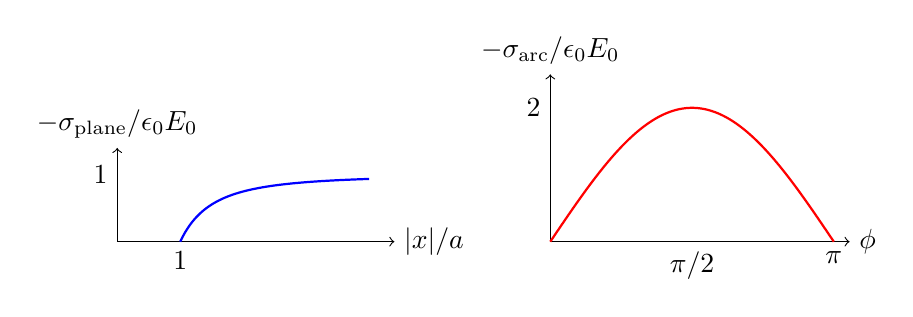
\begin{tikzpicture}[x=.8cm,y=.85cm]
\draw[->] (0,0)--(4.4,0) node[right] {$|x|/a$};
\draw[->] (0,0)--(0,1.4) node[above] {$-\sigma_{\rm plane}/\epsilon _0E_0$};
\draw[thick,blue,domain=1:4,samples=80] plot (\x,{1-1/(\x^2)});
\node[below] at (1,0) {$1$};\node[left] at (0,1) {$1$};
\begin{scope}[xshift=5.5cm,x=.02cm]
\draw[->] (0,0)--(190,0) node[right] {$\phi$};
\draw[->] (0,0)--(0,2.5) node[above] {$-\sigma_{\rm arc}/\epsilon _0E_0$};
\draw[thick,red,domain=0:180,samples=80] plot (\x,{2*sin(\x)});
\node[below] at (90,0) {$\pi/2$};\node[below] at (180,0) {$\pi$};
\node[left] at (0,2) {$2$};
\end{scope}
\end{tikzpicture}
\end{center}
The arc charge per unit $z$ length is
\[
Q_{\rm arc}=-2\epsilon _0E_0a\int_0^\pi\sin\phi\,d\phi
=-4\epsilon _0E_0a,
\]
twice the charge $-2\epsilon _0E_0a$ on the displaced flat strip.
The deficit in charge magnitude on the remaining plane is
\[
2\int_a^\infty[\sigma_{\rm plane}(x)+\epsilon _0E_0]\,dx
=2\epsilon _0E_0a^2\int_a^\infty\frac{dx}{x^2}
=2\epsilon _0E_0a,
\]
exactly the negative of the extra arc charge. More precisely, the
charge on the arc plus the plane portions $a<|x|<L$ is
\[
Q_L=-2\epsilon _0E_0L-\frac{2\epsilon _0E_0a^2}{L}.
\]
Compared with the flat value $-2\epsilon _0E_0L$, the relative
change is $a^2/L^2\to0$ for a wide strip.

\Needspace{5\baselineskip}
\par\bigskip
\noindent\textbf{2.27}\quad Consider the two-dimensional wedge-shaped region of Problem 2.26, with $\beta=2\pi$. This corresponds to a semi-infinite thin sheet of conductor on the positive $x$ axis from $x=a$ to infinity with a conducting cylinder of radius $a$ fastened to its edge.
\begin{enumerate}
\item[(a)] Sketch the surface-charge densities on the cylinder and on the top and bottom of the sheet, using the lowest order solution.
\item[(b)] Calculate the total charge on the cylinder and compare with the total deficiency of charge on the sheet near the cylinder, that is, the total difference in charge for $a$ finite compared with $a=0$, assuming that the charge density far from the cylinder is the same.
\end{enumerate}
\solution
For $\beta=2\pi$ the lowest angular index is $\nu=1/2$.
Let its coefficient $A$ be positive; all signs reverse if $A<0$.
The potential near the cylinder is
\[
\Phi=A\left(\sqrt\rho-\frac a{\sqrt\rho}\right)\sin\frac\phi2.
\]
\textbf{(a)} The formulas of Problem 2.26 give
\[
\boxed{\sigma_{\rm cylinder}(\phi)=-\frac{\epsilon _0A}{\sqrt a}
                              \sin\frac\phi2,\quad0<\phi<2\pi,}
\]
\[
\boxed{\sigma_{\rm top}(x)=\sigma_{\rm bottom}(x)
 =-\frac{\epsilon _0A}{2\sqrt x}\left(1-\frac ax\right),\quad x>a.}
\]
The density on the cylinder vanishes at the attachment point and
is largest in magnitude at the leftmost point, $\phi=\pi$.
Each sheet face starts from zero at $x=a$, reaches its largest
magnitude at $x=3a$ (differentiate $x^{-1/2}-ax^{-3/2}$), and then
approaches the $a=0$ edge law $-\epsilon _0A/(2\sqrt x)$.
The normalized maximum sheet magnitude is $1/(3\sqrt3)$ in units
$\epsilon _0A/\sqrt a$.
\begin{center}
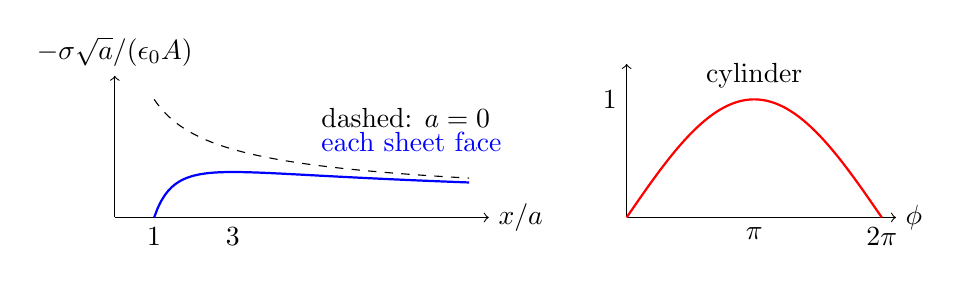
\begin{tikzpicture}[x=.5cm,y=3cm]
\draw[->] (0,0)--(9.5,0) node[right] {$x/a$};
\draw[->] (0,0)--(0,.6) node[above] {$-\sigma\sqrt a/(\epsilon _0A)$};
\draw[blue,thick,domain=1:9,samples=90] plot (\x,{(1-1/\x)/(2*sqrt(\x))});
\draw[dashed,domain=1:9,samples=90] plot (\x,{1/(2*sqrt(\x))});
\node[below] at (1,0) {$1$};\node[below] at (3,0) {$3$};
\node[right] at (5,.42) {dashed: $a=0$};
\node[blue,right] at (5,.32) {each sheet face};
\begin{scope}[xshift=6.5cm,x=.009cm,y=1.5cm]
\draw[->] (0,0)--(380,0) node[right] {$\phi$};
\draw[->] (0,0)--(0,1.3);
\draw[red,thick,domain=0:360,samples=90] plot (\x,{sin(\x/2)});
\node[below] at (180,0) {$\pi$};\node[below] at (360,0) {$2\pi$};
\node[left] at (0,1) {$1$};\node at (180,1.2) {cylinder};
\end{scope}
\end{tikzpicture}
\end{center}
\textbf{(b)} Integration on the full circular surface gives
\[
Q_c=-\epsilon _0A\sqrt a\int_0^{2\pi}\sin\frac\phi2\,d\phi
=\boxed{-4\epsilon _0A\sqrt a}.
\]
Although the total charge of an infinite sheet diverges, the
difference between the two configurations is integrable. On the
part $x>a$ that remains in both configurations,
\[
\Delta Q_{x>a}=2\int_a^\infty
  \frac{\epsilon _0Aa}{2x^{3/2}}\,dx=2\epsilon _0A\sqrt a.
\]
The reference sheet also had the part $0<x<a$, on both faces,
which has now been replaced by the cylinder. Its removed charge is
\[
Q_{0<x<a}^{(0)}=2\int_0^a-\frac{\epsilon _0A}{2\sqrt x}\,dx
=-2\epsilon _0A\sqrt a.
\]
Thus the \emph{total} sheet deficiency is
$\Delta Q_{\rm sheet}=2\epsilon _0A\sqrt a-(-2\epsilon _0A\sqrt a)
=4\epsilon _0A\sqrt a=-Q_c$.
Omitting the removed strip would count only half the deficiency.

\Needspace{5\baselineskip}
\par\bigskip
\noindent\textbf{2.28}\quad A closed volume is bounded by conducting surfaces that are the $n$ sides of a regular polyhedron ($n=4$, 6, 8, 12, 20). The $n$ surfaces are at different potentials $V_{i}$, $i=1,2,\ldots,n$. Prove in the simplest way you can that the potential at the center of the polyhedron is the average of the potential on the $n$ sides. This problem bears on Problem 2.23b, and has an interesting similarity to the result of Problem 1.10.
\solution
Let $u_i(\mathbf x)$ solve Laplace's equation with boundary value
one on face $i$ and zero on the other faces. By linearity and
Dirichlet uniqueness,
\[
\Phi(\mathbf x)=\sum_{i=1}^nV_i u_i(\mathbf x).
\]
A symmetry of a regular polyhedron carries any face into any other
while leaving its center $\mathbf x_c$ fixed. Applying that symmetry
to a unit-face solution and using uniqueness therefore proves
$u_i(\mathbf x_c)=u_j(\mathbf x_c)$ for all $i,j$.
Moreover, $\sum_i u_i$ has boundary value one on every open face,
so its unique interior solution is the constant one. At the center,
\[
1=\sum_i u_i(\mathbf x_c)=n u_i(\mathbf x_c).
\]
It follows immediately that
\[
\boxed{\Phi(\mathbf x_c)=\frac1n\sum_{i=1}^nV_i.}
\]
Idealized voltage jumps on shared edges can be understood as limits
of narrow insulating gaps; the interior harmonic solution is
unaffected by the assignment of boundary values on the edges alone.
The proof uses face-transitive symmetry, not a general assertion
that the potential equals an area average on an arbitrary enclosing
surface. For the cube of Problem 2.23, two of its six faces contribute,
so the center potential is $V/3$.

\Needspace{5\baselineskip}
\par\bigskip
\noindent\textbf{2.29}\quad For the Galerkin method on a two-dimensional square lattice with lattice spacing $h$, verify the relations (2.81) for the localized ``pyramid'' basis functions, $\phi_{ij}(x,y)=(1-|x|/h)(1-|y|/h)$, $|x|<h$, $|y|<h$, where $x$ and $y$ are measured from the site $(i,j)$. In particular,
\begin{gather*}
\int dx\int dy\;\phi_{i,j}(x,y) = h^{2};\qquad
\int dx\int dy\;\nabla\phi_{i,j}\cdot\nabla\phi_{i,j} = \frac{8}{3};\\
\int dx\int dy\;\nabla\phi_{i+1,j}\cdot\nabla\phi_{i,j} = -\frac{1}{3};\qquad
\int dx\int dy\;\nabla\phi_{i,j+1}\cdot\nabla\phi_{i,j} = -\frac{1}{3};\\
\int dx\int dy\;\nabla\phi_{i+1,j+1}\cdot\nabla\phi_{i,j} = -\frac{1}{3}
\end{gather*}
\solution
Define a one-dimensional tent
$f(x)=1-|x|/h$ for $|x|<h$, and zero otherwise. Then
$\phi_{ij}(x,y)=f(x-ih)f(y-jh)$, and each required two-dimensional
integral factors into one-dimensional integrals. For a tent and its
nearest translate, direct integration gives
\begin{align*}
I&=\int f(x)\,dx=2\int_0^h(1-x/h)\,dx=h,\\
M_0&=\int f^2\,dx=2\int_0^h(1-x/h)^2\,dx=\frac{2h}{3},\\
M_1&=\int f(x)f(x-h)\,dx
=\int_0^h(1-x/h)(x/h)\,dx=\frac h6,\\
K_0&=\int[f'(x)]^2\,dx=\int_{-h}^h\frac{dx}{h^2}=\frac2h,\\
K_1&=\int f'(x)f'(x-h)\,dx
=\int_0^h\left(-\frac1h\right)\left(\frac1h\right)dx=-\frac1h.
\end{align*}
Supports separated by two or more mesh spacings have zero overlap
except on sets of measure zero. First,
\[
\boxed{\int\phi_{ij}\,dx\,dy=I^2=h^2.}
\]
For any two sites, the gradient product has an $x$-derivative term
and a $y$-derivative term. The coincident-site integral is therefore
\[
\boxed{K_0M_0+M_0K_0=2(2/h)(2h/3)=\frac83.}
\]
For a horizontal neighbor the result is
\[
\boxed{K_1M_0+M_1K_0=-\frac23+\frac13=-\frac13,}
\]
and a vertical neighbor interchanges the two terms with the same
answer. For a diagonal neighbor both coordinates are translated:
\[
\boxed{K_1M_1+M_1K_1=2(-1/h)(h/6)=-\frac13.}
\]
The same values hold for all reflected nearest neighbors. Thus a
row of the interior stiffness matrix has $8/3$ on its own site and
$-1/3$ at each of eight neighboring sites; their sum is zero,
as required for a constant potential to have zero gradient.

\Needspace{5\baselineskip}
\par\bigskip
\noindent\textbf{2.30}\quad Using the results of Problem 2.29, apply the Galerkin method to the integral equivalent of the Poisson equation with zero potential on the boundary,
\[
\int_{V}dx\;dy\,[\nabla\phi_{i,j}\cdot\nabla\psi - 4\pi\rho\,\phi_{i,j}] = 0
\quad\text{with}\quad
\psi(x,y) = \sum_{i',j'=1}^{N}\psi_{i'j'}\,\phi_{i'j'}(x,y)
\]
for the lattice of Problem 1.24, with its three independent lattice sites. Show that you get three coupled equations for the $\psi_{i,j}$ values ($\psi_{1},\psi_{2},\psi_{3}$) and solve to find the ``Galerkin'' approximations for the potential at these sites. Compare with the exact values and the results of the various iterations of Problem 1.24c. Comment.
\[
[\psi = 4\pi\epsilon_{0}\Phi].
\]
\solution
Here $\rho=1$, $h=1/4$, and $\psi=4\pi\epsilon _0\Phi$.
Inserting the basis expansion into the weak equation and using
Problem 2.29 gives
\[
\frac83\psi_{ij}-\frac13\sum_{\text{eight neighbors}}\psi_{i'j'}
=4\pi h^2,
\quad\hbox{or}\quad
8\psi_{ij}-\sum_{\text{eight neighbors}}\psi_{i'j'}=\frac{3\pi}{4}.
\]
Boundary nodes have zero potential. Label the three independent
interior values by their sites in Problem 1.24:
$\psi_1=\psi(1/4,1/4)$,
$\psi_2=\psi(1/2,1/4)$,
$\psi_3=\psi(1/2,1/2)$.
At a corner-type interior site the nonzero neighbors are
$2\psi_2+\psi_3$; at an edge-type site they are
$2\psi_1+2\psi_2+\psi_3$; at the center they are
$4\psi_1+4\psi_2$. Thus
\[
\boxed{\begin{aligned}
8\psi_1-2\psi_2-\psi_3&=3\pi/4,\\
-2\psi_1+6\psi_2-\psi_3&=3\pi/4,\\
-4\psi_1-4\psi_2+8\psi_3&=3\pi/4.
\end{aligned}}
\]
Subtracting the second equation from the first gives
$10\psi_1-8\psi_2=0$, so $\psi_2=5\psi_1/4$.
The first then gives $\psi_3=11\psi_1/2-3\pi/4$.
Substitution into the third gives
$35\psi_1=27\pi/4$. Consequently
\[
\boxed{\psi_1=\frac{27\pi}{140}=0.605878583,\quad
       \psi_2=\frac{27\pi}{112}=0.757348229,\quad
       \psi_3=\frac{87\pi}{280}=0.976137717.}
\]
For comparison, the improved finite-difference equations of
Problem 1.24 are
\[
\begin{pmatrix}20&-8&-1\\-8&18&-4\\-4&-16&20\end{pmatrix}
\begin{pmatrix}\psi_1\\\psi_2\\\psi_3\end{pmatrix}
=\frac{3\pi}{2}\begin{pmatrix}1\\1\\1\end{pmatrix}.
\]
To exhibit the iterations, put $b_0=3\pi/2$. The reduced Jacobi
updates are
\[
\psi_1^{(r+1)}=\frac{b_0+8\psi_2^{(r)}+\psi_3^{(r)}}{20},\quad
\psi_2^{(r+1)}=\frac{b_0+8\psi_1^{(r)}+4\psi_3^{(r)}}{18},\quad
\psi_3^{(r+1)}=\frac{b_0+4\psi_1^{(r)}+16\psi_2^{(r)}}{20}.
\]
Ordered Gauss--Seidel uses the just-computed $\psi_1^{(r+1)}$
in the second equation and both new $\psi_1^{(r+1)},\psi_2^{(r+1)}$
in the third. Solving the three simultaneous equations, for example
eliminating $\psi_3=20\psi_1-8\psi_2-b_0$ from the first, gives
\[
-88\psi_1+50\psi_2=-3b_0,\qquad
396\psi_1-176\psi_2=21b_0.
\]
Their solution is
$(\psi_1,\psi_2,\psi_3)=(783\pi/4312,45\pi/196,159\pi/539)$.
Starting from $(1,1,1)$ and applying Jacobi or ordered Gauss--Seidel
to this reduced matrix (with diagonal $18$ in its second row, as
in Problem 1.24) gives the comparison below.
\begin{center}
\begin{tabular}{lrrr}
\toprule
Method & $\psi_1$ & $\psi_2$ & $\psi_3$\\\midrule
Exact series, Problem 2.16 & .569082647 & .720491684 & .925781529\\
Galerkin, $h=1/4$ & .605878583 & .757348229 & .976137717\\
Jacobi, iteration 2 & .668786843 & .841101243 & 1.115516182\\
Jacobi, iteration 6 & .587144572 & .743033367 & .960088859\\
Jacobi, iteration 10 & .573384927 & .725179706 & .932570355\\
Gauss--Seidel, iteration 2 & .601302817 & .752097624 & .957558112\\
Gauss--Seidel, iteration 6 & .571530449 & .722284498 & .927753137\\
Gauss--Seidel, iteration 10 & .570504738 & .721316714 & .926773768\\
Improved stencil, converged & .570470095 & .721284028 & .926740690\\
\bottomrule
\end{tabular}
\end{center}
The Galerkin values exceed the exact values by approximately
$6.47\%$, $5.12\%$, and $5.44\%$, respectively, whereas the converged
improved stencil errors are $0.244\%$, $0.110\%$, and $0.104\%$.
This comparison separates the error in solving a discrete system
from its spatial approximation error: more iterations converge to
the stencil's fixed solution, not to the continuum solution. The
Galerkin calculation is also a different discrete approximation,
using piecewise bilinear tents and a variational integral; on this
coarse grid it is less accurate at these nodes. This is not a general
failure of finite elements: mesh refinement, or richer basis functions,
changes that approximation. Galerkin stationarity controls the
integrated field-energy error, not the sign or size of each nodal
potential error.
